\documentclass{customgost}



%%%%%%%%%%%%%%%%%%%%%%%%%%%%%%%%%%%%%%%%%%%%%%%%%%%%%%%%%%%%%
% Настройки титулки
\usepackage{unn-titlepage}
\TitleWorkTitle{Оценка угловой координаты источника излучения в 
мобильных системах связи миллиметрового диапазона \\ длин волн}

\setauthor{1}{Зав. кафедрой статистической радиофизики  \\ и мобильных систем связи,  \\ профессор, д.ф.–м.н.}{Мальцев А.А.}
\setauthor{2}{Научный руководитель,  \\ профессор, д.ф.-м.н}{Мальцев А.А.}
\setauthor{3}{Рецензент,  \\ доцент, к.ф-м.н.}{Михеев П.В.}
\setauthor{4}{Консультант по технике безопасности,  \\ доцент, к.ф.-м.н.}{Клемина А.В.}
\setauthor{5}{Студент 4-го курса магистратуры}{Понур К.А.}
%%%%%%%%%%%%%%%%%%%%%%%%%%%%%%%%%%%%%%%%%%%%%%%%%%%%%%%%%%%%%




% Для псевдокода
%%%%%%%%%%%%%%%%%%%%%%%%%%%%%%%%%%%%%%%%%%%%%%%%%%%%%%%%%%%%%
\usepackage{algorithm}
\usepackage{algpseudocode} 
\floatname{algorithm}{Алгоритм}
%%%%%%%%%%%%%%%%%%%%%%%%%%%%%%%%%%%%%%%%%%%%%%%%%%%%%%%%%%%%%

% Настройки номенклатуры
%%%%%%%%%%%%%%%%%%%%%%%%%%%%%%%%%%%%%%%%%%%%%%%%%%%%%%%%%%%%%
\usepackage{nomencl}
\usepackage{multicol}
\usepackage{etoolbox}
\renewcommand\nomgroup[1]{%
\item[\bfseries
\ifstrequal{#1}{A}{Сокращения}{%
\ifstrequal{#1}{B}{Обозначения}{%
\ifstrequal{#1}{C}{}{}}}%
]}
\newcommand{\nomunit}[1]{%
\renewcommand{\nomentryend}{\hspace*{\fill}#1}}
\renewcommand{\nompreamble}{\footnotesize\begin{multicols}{2}}
\renewcommand{\nompostamble}{\end{multicols}}
\renewcommand{\nomname}{Обозначения и сокращения}
\makenomenclature  
\makeindex
%%%%%%%%%%%%%%%%%%%%%%%%%%%%%%%%%%%%%%%%%%%%%%%%%%%%%%%%%%%%%






% Прочее
\newcommand\mean[1]{\langle #1 \rangle}
\newcommand\const{\text{const}}
\renewcommand{\phi}{\varphi}
\renewcommand{\epsilon}{\varepsilon}
\renewcommand\vec[1]{\vectorbold{#1}}
\setcounter{MaxMatrixCols}{20}

% Настройка переносов некоторых слов
\hyphenation{при-ем-ни-ков}

\addbibresource{library.bib}
\usepackage{enumitem}
\usepackage{subcaption}
\usepackage{soulutf8}



% \titlecontents{chapter}[0pt\addvspace{15pt}]
% {\llap{\makebox[3em]{\oldstylenums{\thecontentspage\hfill\thecontentslabel}}\hskip1em}
%   \small\scshape\vskip-\baselineskip}{}{}{}
% \titlecontents*{section}[20pt]
% {\upshape}{}{}
% {, \oldstylenums{\thecontentspage}}[][\ \textbullet\ ][]
\begin{document}



\maketitle
\newpage

\tableofcontents
\newpage
\nomenclature[A]{LLS}{Link Level Simulator}
\nomenclature[A]{УМ}{Усилитель Мощности}
\nomenclature[A]{КУ}{Коэффициент Усиления}
\nomenclature[A]{АХ}{Амплитудная Характеристка}
\nomenclature[A]{ФХ}{Фазовая Характеристка}
\nomenclature[A]{OBO}{Output Back-Off}
\nomenclature[A]{IBO}{Input Back-Off}
\nomenclature[A]{5G NR}{5G New Radio}
\nomenclature[A]{OFDM}{Orthogonal Frequency Division Multiplexing}
\nomenclature[A]{CP}{Cyclic Prefix}
\nomenclature[A]{PD}{Pre-Distortion}
% \nomenclature[A]{AATLF}{Adaptive Angle Tracking Loop Filter}
% \nomenclature[A]{AIC}{Akaike’s Information Criterion}
% \nomenclature[A]{AIP}{Antenna in Package}
% \nomenclature[A]{AOA}{Angle of Arrival}
% \nomenclature[A]{AOD}{Angle of  Departure}
% \nomenclature[A]{AWGN}{Additive White Gaussian Noise}
% \nomenclature[A]{BRP}{Beam Refinement Protocol}
% \nomenclature[A]{CCATLF}{Constant Coefficient Angle Tracking Loop Filter}
% \nomenclature[A]{CDF}{Cumulative Distribution Function}
% \nomenclature[A]{CFAR}{Constant False Alarm Ratio}
% \nomenclature[A]{CoMP}{Coordinated Multipoint}
% \nomenclature[A]{CSI}{Channel State Information}
% \nomenclature[A]{DCO}{Digitally Controlled Oscillator}
% \nomenclature[A]{DKED}{Double Knife-Edge Diffraction}
% \nomenclature[A]{DVR}{Digital Video Recorder}
% \nomenclature[A]{EG}{Equal Gain}
% \nomenclature[A]{EKF}{Extended Kalman Filter}
% \nomenclature[A]{FFT}{Fast Fourier Transform}
% \nomenclature[A]{GCS}{Global Coordinate System}
% \nomenclature[A]{HBF}{Hybrid Beamforming}
% \nomenclature[A]{HDTV}{High Definition Television}
% \nomenclature[A]{KF}{Kalman Filter}
% \nomenclature[A]{LCS}{Local Coordinate System}
% \nomenclature[A]{LF}{Loop Filter}
% \nomenclature[A]{LOS}{Line-of-Sight}
% \nomenclature[A]{MDL}{Minimum Description Length}
% \nomenclature[A]{ML}{Maximum Likelihood}
% \nomenclature[A]{MMSE}{Minimal Mean Square Error}
% \nomenclature[A]{MPM}{Minimal Polynomial Method}
% \nomenclature[A]{MS}{Maximal Selection}
% \nomenclature[A]{MUSIC}{MUltiple SIgnal Classification}
% \nomenclature[A]{MVDR}{Minimum Variance Distortionless Response}
% \nomenclature[A]{NLOS}{Non Line-of-Sight}
% \nomenclature[A]{NR}{New Radio}
% \nomenclature[A]{PBCH}{Physical Broadcast Channel}
% \nomenclature[A]{PDF}{Probability Density Function}
% \nomenclature[A]{PSS}{Primary Synchronization Signal}
% \nomenclature[A]{RGB-D}{Red-Green-Blue-Depth}
% \nomenclature[A]{RS}{Reference Signal}
% \nomenclature[A]{SLS}{Sector Level Sweep}
% \nomenclature[A]{SSS}{Secondary Synchronization Signal}
% \nomenclature[A]{SVD}{Singular Value Decomposition}
% \nomenclature[A]{TDM}{Time Division Multiplexing}
% \nomenclature[A]{ULA}{Uniform Linear Array}

\printnomenclature
\newpage

%! TeX root = ../main.tex
\Introduction

Развитие стандарта мобильной связи 5G New Radio (NR), разрабатываемого консорциумом
3GPP (3rd Generation Partnership Project), тесно связано с развитием
технологии Интернета Вещей (IoT - Internet of Things). Высокая скорость,
надежность сети, малая задержка, а также возможность массового подключения
"умных" устройств являются важнейшими параметрами, определяющими
производительность системы в целом.

Одни из последних релизов стандарта 5G NR - релизы 15 и 16 обеспечивают
поддержку несущих частот до 52.6 ГГц. С целью расширить поддержку текущего
частотного диапазона FR2 (\textit{Англ. - Frequency Range 2}) до 52.6 - 71 ГГц с
минимальными вносимыми изменениями в систему \cite{intel193259}
\cite{qlcm193229}, группа RAN проекта 3GPP уже исследовала требования для
диапазона 52.6 - 114.25 ГГц \cite{3gpp.38.807}. Помимо этого, была также
исследована возможность расширения частотного диапазона до миллиметровых
волн 71-114 ГГц. Однако в этом диапазоне появляется такое ограничение, как
нелинейный искажения, вызванные работой усилителя мощности (УМ). Несмотря
на значительное продвижение в технологии разработки и проектирования УМ с
использованием новых материалов, все ещё наблюдаются значительные нелинейные
искажения сигнала при использовании стандартной мощности передатчика
\cite{zhang2021}. В данном диапазоне частот УМ может внести значительные
искажения, кардинально снизив производительность
системы. Это особенно заметно для высокоэффективных модуляций, например,
64-QAM и 256-QAM.

Данным эффектом искажения сигнала можно пренебречь в низких диапазонах
частот, таких как FR1 и частично FR2. Рабочую точку УМ в этих диапазонах
можно выбрать таким образом, что на выходе усилителя будет достигаться
необходимая выходная мощность, и при этом УМ будет работать в линейной
области своей характеристики, что минимизирует вносимые в передаваемый
сигнал искажения.

Проблема искажения сигнала на высоких частотах наиболее актуальна а рамках
рассмотрения использования стандарта связи 5G NR в применении к технологии
Интернета Вещей. В данном случае система имеет огромное количество
небольших и простых передающих устройств, таких как датчики, сенсоры, а
также прочие устройства, используемые для обеспечения тесно
связанного окружения. Подобные элементы часто имеют низкокачественные
передающие и усилительные цепи ввиду необходимости общей низкой стоимости
прибора. Также данные устройства должны быть энергоэффективными и
минимизировать общее потребление электроэнергии для возможности создания
инфраструктуры из большого количества отдельных компонент.
Эти факторы являются ключевыми при выборе метода компенсации вносимых
нелинейных искажений, поскольку вспомогательная обработка на передатчике
может внести дополнительные энергозатраты, нежелательные для дешевого,
энергоэффективного устройства.

Проблема компенсации нелинейных искажений, вносимых УМ, рассматривалась во
многих работах, в том числе для низких диапазонов частот
\cite[]{sharath2015,shabany2008,eda2001,maltsev2021,bhat2016,qi2010,gregorio2007}.
Рассматривались различные подходы, в основе которых лежали предварительное
искажение (\textit{Англ. - Pre-Distortion (PD), Digital Pre-Distortion
(DPD)}) сигнала на передатчике с целью "выпрямления" амплитудной
характеристики усилителя. Однако такие методы требуют дополнительной
сигнальной обработки на передатчике, что негативно влияет на
энергоэффективность устройства. В основе другого метода лежит обработка
сигнала на приемнике, когда принятый сигнал подвергается обработке на
стороне принимающего устройства с целью компенсации искажений, внесенных на
УМ передатчика. В качестве методов компенсации используют обратную
характеристику УМ, статистические подходы для определения усредненного
искажения и его дальнейшей компенсации, последовательный метод Монте-Карло
и другие. Также важно отметить необходимость в определенных случаях знать
на приемнике параметры УМ, который расположен на передатчике.

Также важно отметить, что характеристики УМ в миллиметровом диапазоне
частот 100-200 ГГц значительно отличаются от характеристик усилителей в
диапазоне 30-70 ГГц. На более высоких частотах, характеристики значительно
хуже, это означает необходимость применения определенного метода
компенсации искажения для повышения качества передачи информации.

В данной работе предлагается метод компенсации нелинейных искажений
внесенных усилителем мощности на приемнике. Основа метода компенсации
заключается в использовании обратной характеристики УМ, однако перед этим
сигнал определенным образом обрабатывается. Предлагаемый метод может быть
использован для разных типов сигналов(CP-OFDM, DFT-s-OFDM),
в зависимости от рассматриваемой задачи. Также, в рамках данной работы были
исследованы характеристики современных твердотельных УМ в миллиметровом диапазоне. На
основе проведенного исследования, была создана модель для диапазона
частот 100-200 ГГц, которая в дальнейшем использовалась в математическом
моделировании для проверки работоспособности предлагаемого метода.



% \textbf{Черновой план диплома}

% \textit{Краткое описание. Скорее для себя, чтобы самому не забыть в чем
% основная суть работы, в дипломе этого не будет}

% \begin{itemize} \item 5G расширяется и активно исследует суб-ТГц диапазон
%     \item усилители в этом диапазоне не очень, много искажений
%     \item особенно для маленьких дешевых устройств, где важна
%     энергоэффективность
%     \item нужна обработка на приемнике
%     \item предлагаемый метод обработки
%     \item краткий план-содержание работы
%     \end{itemize}





% Дипломная работа о разработке метода компенсации нелинейных искажение
% сигнала на приемнике, возникших в результате работы усилителя мощности на
% передатчике. Усилитель имеет нелинейную амплитудную характеристику, что и
% является причиной искажения сигнала.

% Учитывая планы расширения стандарта 5G в суб-терагерцовый диапазон,
% нелинейность характеристики УМ в этих частотах только ухудшается,
% значительно снижая эффективность системы в целом. Это является основным
% мотивом разработки метода компенсации вносимых передатчиком искажений на
% приемнике.

% Также, компенсация рассматривается именно на приемнике, поскольку в таком
% случае передатчику не нужно производить дополнительную обработку сигнала,
% что важно для энергопотребления. Такой метод может использоваться в
% системах с большим количеством мало-размерных, простых передатчиков,
% которые часто используются в системе интернета вещей.

% \section{Введение (5G, IoT, sub-THz range, PA nonlinearity)}


% \section{Роль усилителя мощности и влияние нелинейности амплитудной
% характеристики} \subsection{Описание принципа работы усилителя мощности}
% \subsection{Влияние нелинейности и искажение различных сигналов на
% приемнике} \subsubsection{Искажение сигнала SC} \subsubsection{Искажение
% сигнала CP-OFDM} \subsubsection{Искажение сигнала DFT-s-OFDM}
% \subsection{Характеристики усилителей в суб-ТГц диапазоне}
% \subsection{Обзор существующих моделей для описания усилителя мощности}
% \subsubsection{Модель Rapp} \subsubsection{Новая модель для диапазона
% частот 100-200 ГГц}

% \section{Метод компенсации нелинейных искажений на приемнике}
% \subsection{Краткое описание принципа работы симулятора канального
% уровня} \subsection{Подход и описание нового метода компенсации
% нелинейных искажений} \subsubsection{Адаптация алгоритма компенсации в
% зависимости от типа используемого сигнала} \subsubsection{Компенсация с
% использованием обратной характеристики усилителя}

% \section{Результаты расчетов и симуляций} \subsection{Модель усилителя
% мощности в диапазоне 30-70 ГГц} \subsection{Модель усилителя мощности в
% диапазоне 100-200 ГГц}

% \section{Заключение}

% \section{Приложение}

% \newpage
% \Introduction

% \textit{В введении указывается актуальность темы, цели и задачи исследования, предметы и
% методы исследования, теоретическую и практическую значимость, научная новизна,
% положения, выносимые на защиту, краткое описание структуры работы.}


% В последние годы Интернет Вещей (IoT), поддерживаемый технологией 5G,
% стремительно развивался в широком спектре применений, обеспечивая связь
% между объектами в автомобильной индустрии, бытовой электронике,
% транспортном, логистическом и производственном секторе. С ростом
% повсеместной интеграции и использования различных малогабаритных
% датчиков, стоимость производства каждого отдельно взятого элемента
% остается критическим аспектом. Относительно низкая цена отдельных
% элементов является ключом к созданию тесно связанной среды, однако это
% может серьезно повлиять на качество радиочастотных цепей, а также на
% общую производительность системы. С расширением 5G до субтерагерцовых
% диапазонов, нелинейные искажения усилителя мощности (УМ) могут
% значительно ограничить производительность системы даже в
% высококачественных устройствах из-за конструктивных ограничений
% усилителя. Было проведено множество исследований с целью уменьшения
% влияние нелинейности как на стороне передатчика, так и на стороне
% приемника. Многие решения предлагают определенные варианты оценки
% эффектов УМ посредством обратной связи, направленной на принятие решения,
% обучения или даже статистической обработки полученного сигнала. Однако,
% зная функцию нелинейности УМ на приемной стороне, обработка может быть
% упрощена до применения обратной функции к эквивалентному сигналу во
% временной области.

% В этой работе мы предлагаем метод компенсации нелинейных искажений УМ на
% стороне RX, который можно настроить для нескольких форм сигналов, таких
% как CP-OFDM и DFT-S-OFDM. Приведенные результаты моделирования
% демонстрируют улучшение характеристик как для субтерагерцовых моделей УМ,
% так и для моделей в диапазоне 30-70 ГГц со значительно лучшими
% характеристиками.



% \section{Описание проблемы и предшествующие решения}
% \textbf{введение из статьи}

% Последние релизы стандарта 5G New Radio (NR) Rel15 и Rel16 поддерживают
% частоты несущих до 52.6 ГГц. Рассматривая работу на частоте свыше 52.6
% ГГЦ, группа RAN проекта 3GPP уже  исследовала требования для диапазона
% частот 52.6 – 114.25 ГГЦ [1], с основной целью расширить  поддержку
% текущего диапазона NR FR2 до 52.6-71 ГГЦ с минимальными изменениями в
% системе [2][3]. Также были исследованы возможности дальнейшего расширения
% в суб-терагерцовый диапазон 71-114 ГГц. В этом диапазоне, несмотря на
% значительное продвижения в технологии разработки и создания УМ, все еще
% наблюдается сильные нелинейные искажения для стандартной разрешенной
% мощности передатчика [4]. Таким образом, искажения, вносимые усилителем
% мощности, могут значительно ограничить производительность системы,
% особенно для высокоэффективных модуляций, таких как 64- и 256-QAM.

% В низких диапазонах частот 5G NR, FR1 и частично FR2, нелинейными
% эффектами УМ можно пренебречь в большинстве случаев, поскольку рабочая
% точка может быть расположена в линейной области, позволяя минимизировать
% искажения передаваемого сигнала. Рассматриваемая проблема значительно
% более актуальна для дешевых трансиверов с низкокачественными
% усилительными цепями. Следует заметить, что количество таких устройств
% может быть очень большим, поскольку дешевые устройства обычно
% используются для создания инфраструктуры Интернета вещей. Данная проблема
% была рассмотрена в нескольких работах [5]-[11], даже для низкочастотных
% диапазонов.

% Для описания искажения амплитуды и фазы при использовании твердотельных
% усилителей мощности широко используется модель Раппа. Модифицированная
% модель Раппа, приведенная в уравнении (1), также включена в базовые
% модели спецификации 3GPP \cite{spec38807}.

% \begin{equation} a=b \end{equation}

% насыщения. A,B,q – параметры кривой искажения фазы. is the small signal
% gain, p is the smoothness factor and ?Vsat is the saturation
% voltage/A?B?qare phase distortion curve parameters.

% Базовые характеристики стандартных УМ в диапазоне частот 30-70 ГГц были
% использованы для вывода математической модели [15], справедливой в
% соответствующей полосе. Однако основываясь на недавних работах
% [4][16][17], можно отметить что характеристики Суб-ТГц УМ даже в полосе
% частот 100-200 ГГц значительно отличаются. Для оценки производительности
% системы для данного диапазона несущих частот, нами была выведена
% усредненная модель УМ на основ последних исследований. Сравнение моделей
% приведено на Figure 1. Основываясь на усредненных параметрах ???, была
% получена модель УМ для диапазона частот 100-200 ГГц.

% На Figure 2 приведены примеры искажения сигнала в следствии действия
% нелинейности УМ для разных видов сигнала. Можно отметить, что для сигнала
% с одной несущей (single carrier - SC), искажения носят детерминированный
% характер в виде амплитудного искажения, которое можно с относительной
% легкостью компенсировать. Однако для сигнала OFDM, нелинейность УМ
% приводит к интерференции между несущими, что результирует в случайном
% характере искажения, которое намного сложнее компенсировать.

% DFT spread OFDM (DFT-s-OFDM) представляет некую промежуточную ситуацию,
% когда присутствуют как и детерминированный характер искажения, так и
% случайный, позволяя произвести компенсацию нелинейности.

% На данный момент существуют два различных подхода для компенсации
% нелинейности УМ. Первый заключается в предварительном искажении сигнала
% перед УМ на передатчике, придавая сигнал определенные свойства,
% минимизирующие влияние нелинейного искажения от УМ. Существует множество
% вариантов обработки для данного подхода, однако все они имеют слабый
% эффект на общей производительности системы, а предварительное искажение
% имеет низкую эффективность на низких значениях IBO [5][6][7].
% Использование предварительного искажения  на передатчике нежелательно и
% на мало-габаритных устройствах, поскольку в этом случае растет объем
% сигнальной обработки, что увеличивает энергопотребление.

% Второй подход заключается в компенсации нелинейных искажений на
% приемнике. Например, в [8] используется статистическая обработка
% принятого сигнала для определения средней степени искажения, что
% используется для дальнейшей компенсации. Работы [5][6][9][10][11][12][13]
% рассматривают теоретический подход для компенсации на приемнике в очень
% обобщенном случае. Несколько методов компенсации влияния нелинейности УМ
% были предложены для OFDM сигнала [11][12][13], где влияние нелинейности
% представляется постоянным комплексным множителем, а также Гауссовой
% шумовой компонентой. Основной задачей в таком случае является определение
% параметров УМ (могут быть как известны изначально, так и определены с
% помощью пилотных сигналов) для компенсации нелинейного искажения.
% Несколько методов были использованы для сигнала SC с одной несущей
% [5][6][9][10], включая….??..., последовательный метод Монте-Карло, а
% также обратную характеристику УМ. В нескольких случаях [9][11][10],
% значения параметров УМ считаются известными на приемнике, что позволяет
% произвести компенсацию искажения. В случаях, когда параметры УМ
% оцениваются, производительность такая же либо хуже.

% \section{Новая идея}

% Как было показано для сигнала SC, и, не менее важно, для сигнала
% DFT-s-OFDM, искажения в результате влияния нелинейности УМ имеют
% детерминированный характер, в добавок к ICI. Зная нелинейную
% характеристику, становится возможным компенсировать детерминированную
% компоненту искажений, улучшая итоговую демодуляцию. Этого можно добиться
% применяя обработку сигнала на приемнике, эквивалентную обратной
% характеристике УМ.

% Обычно, эта функция не известна на приемнике не только потому что
% значения параметров УМ не известны, но и в следствии различных значений
% мощности передатчика. Значение этой мощности напрямую влияет на рабочую
% точку УМ, а значит и на то, как искажается конечный сигнал.

% В нескольких работах [10][11][12], the decision-directed feedback??
% используется для оценки характеристики усилителя мощности. Также, в [8]
% используется статистическая обработка для корректировки алгоритма
% демодуляции принятого искаженного сигнала.

% Однако, более эффективным подходом является использование знаний о
% параметрах УМ, а также его рабочей точки для соответствующей пост
% обработки.

% \subsection{Предлагаемый метод компенсации на приемнике} Ниже приведен
% метод компенсации нелинейных искажений УМ на стороне приемника для
% сигнала CP-OFDM, основанный на использовании обратной амплитудной
% характеристики УМ (Figure 3). 

% Схема компенсации состоит из базовой обработки на передатчике (1),
% которая может включать MIMO прекодинг и transform прекодинг (в случае
% DFT-s-OFDM сигнала),  а также стандартного для OFDM блока обратного
% преобразования Фурье. Сгенерированный OFDM сигнал подается на одну или
% более передающих цепочек, которые могут включать добавление цикличного
% префикса, перенос сигнала на несущую частоту, и, наконец, сигнал подается
% на усилитель мощности (2), работающий на несущей частоте. Отметим, что
% для корректной работы предлагаемой схемы, сигналы на разных антеннах
% должны иметь одинаковую амплитуду (но могут иметь разную фазу). Это
% ограничивает применение данного метода до передачи 1 ранга, даже если
% используется несколько передающих антенн. После прохождения через канал,
% сигнал попадает на приемную цепь состоящую из одной или нескольких
% приемных антенн для дальнейшей обработки (4), которая может состоять из
% преобразования Фурье further maximum ration combining (MRC) and frequency
% domain equalization???. Такая обработка эффективно нивелирует влияние
% частотно-селективного канала, что позволяет использовать обработанный
% сигнал на блоке компенсации нелинейного искажения (5). Этот блок может
% состоять из операции обратного Фурье преобразования (6) для возвращения
% сигнала во временную область, блока обратной нелинейной функции УМ (7),
% который выполняет компенсацию нелинейного искажения, а также блока
% прямого преобразования Фурье для возвращения сигнала в частотную область.

% \subsection{Предположения и результаты симуляции} Для проверки
% эффективности предлагаемого метода, были произведены симуляции канального
% уровня, в которых предложенный метод сравнивался со случаями идеального
% УМ, а также отсутствии компенсации на приемнике для совпадающей модели
% усилителя. Использовалась модель основанная на параметрах существующих
% усилителей мощности в диапазоне частот 30-70 ГГц [15], а также модель для
% 100-200 ГГц полученная в результате данной работы. Расчеты проводились
% для различных параметров системы, таких как расстояние между поднесущими
% (SCS), типом используемого сигнала, кодирование, модуляция и другие.
% Полный список параметров симуляции приведен в Table 1.

% \subsection{Последовательность применения компенсаций} Предложенный метод
% предполагается использовать до компенсации фазового шума (PN), однако
% другие последовательности были рассмотрены и рассчитаны. Применение
% компенсации нелинейности УМ после компенсации PN показало определенное
% ухудшение производительности, поэтому компенсация нелинейности УМ везде
% производилась до компенсации фазовых шумов в большинстве расчетов.
% Примеры результатов, в которых сравнивается разный порядок компенсации
% фазовых шумов и нелинейности усилителя приведены на Figure 10.

% \subsection{Наблюдения}

% • Для модели УМ в диапазоне 30-70 ГГц (подходящего для диапазона АК2 и
% выше) улучшение наблюдается только для модуляций высокого порядка o Для
% SCS 120 кГц, отрицательные эффекты фазового шума значительны, и при таких
% искажениях результаты компенсации нелинейности УМ незначительны o Для SCS
% 480 и 960 кГц, в которых возможна более эффективная компенсация фазового
% шума, в определенный момент влияние нелинейности УМ становится основным
% ограничивающим фактором. В этом случае компенсация нелинейности УМ может
% улучшить результат на несколько дБ или совсем избавиться от искажений,
% внесенных УМ. • Для модели 100-200 ГГц, влияние нелинейности УМ
% увеличивается, и в большинстве случаев превосходит влияние фазовых шумов
% o Предложенный метод компенсации демонстрирует улучшение результата для
% MCS 22 и выше • Не смотря на возможность различных имплементаций,
% диктуемая логикой последовательность компенсации искажений в порядке,
% обратному их появлению в системе оказывается оптимальным. Таким образом,
% искажения должны быть компенсированы в порядке канал, усилитель мощности,
% фазовые шумы.  

% \section{Заключение}

% Описан и продемонстрирован метод для компенсации нелинейных искажений
% усилителя мощности на стороне приемника. В основе метода лежит
% использование обратной амплитудной характеристики усилителя, метод может
% быть применен для нескольких различных типов сигнала и подстроен для
% рассматриваемой задачи. Компенсация была реализована и протестирована на
% симуляторе канального уровня, соответствующего требованиям стандарта 5G
% NR для оценки влияния на производительность системы. Метод применялся для
% существующей модели УМ в диапазоне частот 30-70 ГГц, а также для новой
% модели 100-200 ГГц, основанной на последних исследованиях. В обоих
% случаях, предлагаемый метод продемонстрировал возможность значительно
% улучшить производительность системы в различных условиях (вид сигнала,
% модуляция и др.). Поскольку метод опирается на компенсацию на стороне
% приемника, этот подход может быть эффективен в системе с большим
% количеством простых, дешевых передатчиков с низким энергопотреблением.
% Это позволит устройству передачи снизить общее энергопотребление,
% поскольку в таком случае отсутствует необходимость в предварительной
% обработке сигнала для компенсации нелинейных эффектов усилителя.


%! TeX root = ../main.tex
\section{Обзор методов оценки угла прихода}
\label{sec:review}

\subsection{Характеристики канала связи миллиметровых длин волн}
Миллиметровая модель канала имеет ряд особенностей, которые описаны во множестве
литературных источников и мировых стандартах \cite{Maltsev2010, Maltsev2017,
    Xu2002, Akdeniz2014, Rappaport2015}. Основные особенности следующие:
\begin{itemize}
    \item Малое влияние дифракции
    \item Высокие потери в канале связи
    \item Потери на шероховатостях отражающих поверхностей
    \item Пути распространения могут быть ассоциированы с геометрическими лучами
\end{itemize}

Последний пункт является наиболее важным с точки зрения алгоритмов оценки AOA.
Также, из этого свойства канала следует, что количество различимых сильных путей
распространения относительно невелико. Это подтверждено результатами
измерений каналов как для внутренних, так и для наружных сценариев.

Например, результаты измерения AOA в помещении представлены на рис.
\ref{fig:3.1}.  На рис. \ref{fig:3.2} представлены уникальные AOA в случае
уличного сценария <<Манхеттен>>. Можно заметить, что среднее число хорошо
различимых независимых путей распространения $\mu=4.7$, что достаточно
мало.



\begin{figure}[ht]
    \centering
    \includegraphics[width=0.6\linewidth]{figs/fig3.1}
    \caption{ Измерение AOA для определения пути распространения в помещении,
        измеренная мощность показана в полярных координатах, $P$ -- максимум
        измеренной мощности. Геометрические лучи показаны только для позиций
        4.2 и 4.4 \cite{Xu2002}.}
    \label{fig:3.1}
\end{figure}

\begin{figure}[ht]
    \centering
    \includegraphics[width=0.8\linewidth]{figs/fig3.2}
    \caption{
        Зависимость числа различимых путей распространения для различных углов азимута и элевации от расстояния между источником и приемником.
        Среднее значение по всем измерениям составило $\mu=4.7$. Измерения проводились с узкой диаграммой направленности в Манхеттене \cite{Rappaport2015}.}
    \label{fig:3.2}
\end{figure}

На основе рассмотренных работ, можно сделать вывод, что в данной модели
канала чаще всего можно выделить несколько сильнейших путей
распространения и определить их AOA.

<<<<<<< HEAD:sections/1-chapter-one.tex
\subsection{Обзор некоторых методов оценки угловой координаты источника излучения}
=======
\subsection{Обзор методов оценки угловой координаты источника излучения}
\label{sec:review}
>>>>>>> main:sections/1-review.tex

Как показано выше, канал в миллиметровом диапазоне можно представить в виде
набора геометрических лучей.  Самые сильные лучи могут быть
использованы для передачи данных. Как правило, диаграмма направленности
антенны формируется по направлению луча прямой видимости (Line of Sight).
Однако в случае не прямой видимости (Non Line of Sight), может быть
выбран самый сильный отраженный геометрический луч. 

Оценка угла прихода, часто рассматривается в задачах
радиолокации.  Для этих задач  давно разработаны алгоритмы и аппаратные реализации
ещё во времена зарождения радиолокации. Эти алгоритмы совершенствовались, с
появлением фазированных антенных решеток.  
Этот может оказаться очень  полезным с учетом  аппаратных ограничений систем
связи 5G NR -- число цифровых портов обычно мало по сравнению с имеющимся
количеством элементов антенной решетки. 

<<<<<<< HEAD:sections/1-chapter-one.tex
Другой набор алгоритмов пришел из задач спектрального анализа.
В них обычно предполагается, что сигнал каждой антенны принимается независимо.
Эти алгоритмы очень эффективны и дают возможность оценить направления на
несколько целей (лучей) одновременно и имеют сверхразрешающую способность, но c другой стороны, они требуют значительных вычислительных ресурсов.  
=======
Другой набор алгоритмов пришел из задач спектрального анализа.  В них обычно
предполагается, что сигнал каждой антенны принимается независимо.  Эти алгоритмы
очень эффективны и дают возможность оценить направления на несколько целей
(лучей) одновременно и имеют сверх разрешающую способность, но с другой стороны,
они требуют значительных вычислительных ресурсов.  
>>>>>>> main:sections/1-review.tex

В этом разделе мы рассмотрим и систематизируем существующие подходы к оценке
АОА, которые нам удалось найти в открытых литературных источниках.  Будут
представлены их преимущества и недостатки.  На этапе моделирования в следующей
части этой работы, мы сократим этот список и выделим наиболее перспективные
методы.

\subsubsection{Методы Фурье и Бартлетта}
\label{sec:3.2.1}

Простейшая алгоритм оценки AOA в зарубежной литературе называется бимформингом \cite{Tuncer2009, Stoica2005} или методом Фурье \cite{Allen2006}.
Основная идея заключается в максимизации мощности, принятой с определенного
направления.

Обозначим сигнал $\vec{y}(t)$ принятой антенной решеткой от некоторого
удаленного источника
\begin{equation}
    \label{eq:3.1}
    \vec{y}(t) = a(t) \vec{s}(\phi_{src}) + \vec{\xi}(t),
\end{equation}
где ${\vec{s}(\phi_{src})}$ -- фазирующий вектор,
$\phi_{src}$ -- угол прихода (AOA); $\vec \xi$ -- вектор шума.
Каждый элемент фазирующего вектора представляется в виде
\begin{equation}
    \qty{\vec{s}(\phi)}_n = \exp{-i(\vec k (\phi), \vec \rho_n)},
\end{equation}
где $\vec k (\phi_{src})$ -- волновой вектор плоской волны, $\vec\rho_n$ радиус-вектор
$n$-го элемента антенны.
В случае эквидистантной антенной решетки, последнее уравнение приведется
к виду
\begin{equation}
    \qty{\vec s(\phi)}_n = \exp{i2\pi\frac{d}{\lambda}\sin(\phi)n},
\end{equation}
где $d$ -- расстояние между элементами антенной решетки, $\lambda$ -- длина
волны излученного сигнала.

Чтобы получить максимальную мощность с некоторого направления $\phi$ необходимо
сформировать соответствующую диаграмму направленности с помощью
весового вектора антенной решетки $\vec w (\phi) = \vec s(\phi)/\rVert(\vec
    s(\phi))\lVert$.  Тогда, можно найти мощность излученного АР сигнала.
\begin{equation}
    p(\phi) = \abs{\vec w^H (\phi) \vec y}^2.
\end{equation}

Оценкой AOA будет являться значение аргумента $\phi$, обеспечивающего максимум функции $p(\phi)$
\begin{equation}
    \phi^* = \arg\max p(\phi)
\end{equation}

\begin{figure}
    \centering
    \includegraphics[width=\linewidth]{figs/fig3.9}
    \caption{ДН для 16-ти элементной эквидистантной линейной
        решетки ($\frac{d}{\lambda}=0.5$), сформированной в направлении $0^\circ$
        \cite{Tuncer2009}. }
    \label{fig:3.9}
\end{figure}

Для фазированной антенной решетки поиск $\phi^*$ может быть реализован во временной
области с помощью сканирования диаграммой направленности. Если количество
приемников (цифровых портов) равно количеству антенных элементов, искомая
функция $p(\phi)$ может быть оценена в цифровой области \cite{Stoica2005}.  В
литературе этот подход также называется методом Бартлетта \cite{Godara2004}.

Функция $p(\phi)$ примет вид
\begin{equation}
    p(\phi) = \frac{\vec s^H(\varphi) \hat{\vec M} \vec s (\phi)}{N^2},
\end{equation}
где $\hat{\vec M}$ -- оценка корреляционной матрицы принятого сигнала
\begin{equation}
    \hat{\vec M} = \frac{1}{L} \sum\limits_{t=1}^{L} \vec y(t) y^H (t)
\end{equation}

% Уровень боковых лепестков может повлиять на оценку AOA при многолучевом распространении. Чтобы уменьшить уровень боковых
% лепестков антенная решетка взвешивается с некоторой оконной функцией, которая
% устанавливает пространственное распределение амплитуды. 
% Наиболее распространены окна Хэмминга, Ханнинга, Бартлетта, Блэкмана,
% Чебышева и Кайзера. Выбор окна всегда компромисс между
% уровнем боковых лепестков (влиянием помех) и шириной главного лепестка
% (пространственным разрешением).  Например, окно Блэкмана обеспечивает самый низкий уровень
% боковых лепестков и самый широкий главный лепесток.  В отличие от других
% фиксированных окон, окна Кайзера и Чебышева обеспечивают некоторую гибкость в
% настройке результирующих свойств диаграммы направленности. Окно Кайзера
% является аппроксимацией оптимального окна, которое максимизирует относительную
% мощность в главном лепестке \cite{Stoica2005}.  Его часто выбирают вместо
% фиксированного окна, потому что оно имеет более низкий уровень
% боковых лепестков, когда он выбран, чтобы иметь ту же ширину основного
% лепестка, что и соответствующее фиксированное окно (или более узкая ширина
% основного лепестка для данного уровня бокового лепестка).  Окно Чебышева имеет
% то свойство, что пиковый уровень боковых лепестков задается
% постоянным.  При этом ограничении окно обеспечивает минимальную ширину главного
% лепестка. Подробное описание различных оконных функций и их сравнительный анализ можно найти
% в \cite{Stoica2005} \cite{Allen2006}. 

\paragraph{Преимущества}%
\begin{enumerate}
    \item Теоретически, метод Фурье и метод Бартлетта являются оптимальными
          решениями для оценки AOA в случае однолучевого канала.
    \item Легко технически реализуется на конечном устройстве и требует мало
          вычислительных мощностей.
\end{enumerate}

\paragraph{Недостатки}%

\begin{enumerate}
    \item На практике, точность поиска снижается.
          Это происходит, во-первых,  потому что производная функции $p(\phi)$
          в направлении на максимум равна нулю и из-за <<плоской>> вершины сложно
          точно определить точку экстремума. Во-вторых, необходимо
          обеспечить высокую дискретизацию по углу для обеспечения приемлемой
          оценки.
    \item Алгоритм может не подойти в случае быстро движущихся пользователей, если поиск реализован с помощью сканирования во временной области.
    \item Метод обеспечивает разрешающую способность, зависящую
          от ширина главного лепестка ДН. Увеличение отношения сигнал/шум (ОСШ) или времени
          сканирования не приведет к качественному улучшению разрешения.  Это делает
          этот подход малопригодным для оценки многолучевого АОА.
    \item В случае нескольких близко расположенных АОА присутствует
          значительная систематическая ошибка.
\end{enumerate}


\subsubsection{Метод максимального правдоподобия}%
\label{sub:metod_maksimal_nogo_pravdopodobiia}
При наличии нескольких путей распространения, оптимальная оценка AOA может быть
получена с помощью максимально правдоподобной оценки (MLE) \cite{Tuncer2009}. 
Рассмотрим модель сигнала:
\begin{equation}
    \label{eq:3.8}
    \vec y(t) = \sum\limits_{q=1}^{J} a_q(t)\vec s(\phi_q) + \vec \xi(t),
\end{equation}
где $J$ число путей распространения; $a_q(t)$ -- комплексная амплитуда $q$-то
луча, $\vec s(\phi_q)$ -- фазирующий;  $\phi_q$ -- угол прихода (AOA) $q$-то
луча и $\xi(t)$ -- вектор белого гауссового шума.

Для этой модели канала критерий МП может быть записан как критерий минимума
среднеквадратичной ошибки (MMSE)
\begin{equation}
    \label{eq:}
    d(\phi_1, \hdots, \phi_J) = \sum\limits_{t}^{} \abs{\vec(t) -
        \sum\limits_{q=1}^{J} a_q(t) \vec s(\phi_q)}^2 \to \min_{\phi_q}.
\end{equation}
Что можно переписать в виде
\begin{equation}
    \label{eq:}
    d(\phi_1, \hdots, \phi_J) = \sum\limits_{t}^{} \vec y^H(t) \vec
    P_\perp(\phi_1, \hdots, \phi_J) \vec y(t) \to \min_{\phi_q},
\end{equation}
\begin{equation}
    \label{eq:}
    \vec P_\perp(\phi_1, \hdots, \phi_J) = \vec E - \vec S(\vec S^H \vec S)^{-1}
    \vec S^H,
\end{equation}
где $\vec P_\perp$ -- проекционная матрица, 
$\vec S = \qty[\vec s(\phi_1) \dots \vec s (\phi_J)]$. 

Минимизация $d(\phi_1, \hdots, \phi_J)$ в общем случае производится численно и
как правило требует больших вычислительных ресурсов для реализации $J$-мерной
минимизации \cite{Tuncer2009}. 


\paragraph{Преимущества}%
\begin{enumerate}
    \item Обеспечивает оптимальное решение в случае нескольких сильных путей распространения.
\end{enumerate}

\paragraph{Недостатки}%
\begin{enumerate}
<<<<<<< HEAD:sections/1-chapter-one.tex
    \item \hl{Digital antenna array is required}
    \item Требует больших вычислительных затрат
=======
    \item Требует большого количества цифровых портов.
    \item Требует больших вычислительных затрат.
>>>>>>> main:sections/1-review.tex
    \item Не позволяет оценить количество доминирующих путей распространения. Если их количество неизвестно, метод становится неоптимальным. 
\end{enumerate}

\subsubsection{Метод моноимпульса}%
\label{sub:monopulse}

Данная разновидность формирования ДН часто называется моноимпульсом и обычно 
используется в радиолокационных системах для задач слежения. 
Этот алгоритм использует разницу между мощностью двух измеренных лучей как метрику для 
оценки AOA \cite{Tuncer2009}. Вводится следующая функция 
\begin{equation}
    \label{eq:3.11}
    b(\phi) = \frac{1}{\Delta} \qty(\abs{\vec w^H(\phi+0.5 \Delta)\vec y}^2)
    -
    \qty(\abs{\vec w^H(\phi-0.5 \Delta)\vec y}^2) \approx \dv{p(\phi)}{\phi} ,
\end{equation}
где $p(\phi)$ и $\vec w(\phi)$ были определены в разделе \ref{sec:3.2.1}, $\Delta$ -- некоторый скаляр. Тогда, оценка AOA
заключается в поиске такого угла $\phi$, который обеспечивает нуль функции $b(\phi)$
\begin{equation}
    \label{eq:3.12}
    \phi = \arg\qty{b(\phi) = 0}.
\end{equation}

Величина $\Delta$ может быть порядка ширины луча, но  $b(\phi)$ всё равно будет
хорошо аппроксимироваться производной $p(\phi)$, поскольку $b(\phi)$ почти
линейна в большом диапазоне углов около нуля \cite{Tuncer2009}.  

\begin{figure}[h]
    \centering
    \includegraphics[width=\linewidth]{figs/fig3.11}
    \caption{Зависимость метрики $b(\phi)$ для 16-ти элементной ULA \cite{Tuncer2009}. Направление на источник -- 0 град.}
    \label{fig:3.11}
\end{figure}
% Another variant of the algorithm is often called Monopulse Ratio or Amplitude
% Comparison Monopulse \cite{Mosca1969}. This algorithm requires coherent reception with two
% channels (RF-chains): sum and difference. The sum channel is formed with beam
% pattern which has a maximum for a certain direction. The difference beam
% pattern has a null for this direction. In \cite{Kim2018} the algorithm which uses TDM for
% sum and difference channels is proposed and investigated. It employs cycle
% prefix of OFDM signal to receive two identical signals with different beam
% patterns using a single RF-chain and phased antenna array. This approach seems
% promising, but there are some issues related to phase shifter switching delay
% and multipath propagation influence.
% The metric of monopulse ratio is \cite{Kim2018}
% \begin{equation}
%     \label{eq:}
%     \tan(\frac{N}{4}(\phi_{src} - \phi)) =
%     \frac{Im\qty{\sum\limits_{k} y_d(k) y_s^*(k)}}{\sum\limits_{k}
%         \abs{y_s(k)}^2},
% \end{equation}
% where $\phi_{src}$ is actual  AOA;  $\phi$ is roughly estimated AOA via beam
% sweeping (it is the direction of the sum beam); N is number of antenna
% elements; $y_s(k)$ and  $y_d(k)$ are signals f the sum and difference channels
% respectively.
% \begin{equation}
%     \label{eq:}
%     y_s(t) = a(t) \vec w_s^H \vec s(\phi_{src}) + \vec w_s^H \vec \xi(t)
% \end{equation}
% \begin{equation}
%     \label{eq:}
%     y_d(t) = a(t) \vec w_d^H \vec s(\phi_{src}) + \vec w_d^H \vec \xi(t)
% \end{equation}

% For a linear antenna array the corresponding beamforming vectors are
% \begin{equation}
%     \label{eq:}
%     \qty{\vec w_s (\phi)}_n = \exp{i_2\pi \frac{d}{\lambda}} \sin \phi
% \end{equation}
% \begin{equation}
%     \label{eq:}
%     \qty{\vec w_d (\phi)}_{n < \frac n {N}{2}} = - \exp{i_2\pi n \frac{d}{\lambda}} \sin \phi
% \end{equation}
% \begin{equation}
%     \label{eq:}
%     \qty{\vec w_d(\phi)}_{n\geq \frac{N}{2}} = +\exp{i2\pi \frac{d}{\lambda}
%         \sin \phi (n - 0.5N)},
% \end{equation}

% \begin{figure}[htpb]
%     \centering
%     \includegraphics[width=0.6\linewidth]{figs/fig3.12}
%     \caption{Sum and difference beam patterns for monopulse ratio algorithm
%         \cite{Zhu2016}}
%     \label{fig:}
% \end{figure}

% Monopulse ratio is typically used to estimate a single AOA or resolvable angles
% (far spaced targets which are not located within the same beam). However, there
% are some modifications that use a complex monopulse ratio and allow one to
% detect the multiple targets in a certain beam and estimate their angle
% positions \cite{Luoshengbin2016} \cite{Sherman2011}.  


В \cite{Zhu2016} представлена ещё одна реализация метода моноимпульса, не требующая 
поиска нуля функции \eqref{eq:3.11}
\begin{equation}
    \label{eq:3.19}
    \zeta_n = \frac{p(\eta_n - \delta) - p(\eta_n + \delta)}{p(\eta_n - \delta)
        + p(\eta_n + \delta)} =
    \frac{\sin(\psi - \eta_n)\sin\delta}{1 - \cos(\psi - \eta_n)\cos \delta}
\end{equation}

\begin{equation}
    \label{eq:3.20}
    \psi = \eta_n - \arcsin(
    \zeta_n \frac{\sin\delta}{\sin^2 \delta + \zeta^2_n \cos^2\delta}
    -
    \frac{\zeta_n \sqrt{1-\zeta^2_n} \sin \delta \cos \delta}{\sin^2\delta +
        \zeta^2_n \cos^2 \delta}
    )
\end{equation}
где $\psi_n = 2\pi \frac{d}{\lambda} \sin \phi$ -- обобщенный угол 
главного лепестка с азимутальным направлением $\phi$,  $\eta$ -- центральный угол между двумя лучами моноимпульса, 
$n$ -- индекс лучшей пары лучей, $\delta = \frac{\pi}{N}$, $N$ -- число элементов в АР, $p(\eta)$ 
мощность сигнала, измеренной с луча, направленного на обобщенный угол $\eta$.

\begin{figure}[h]
    \centering
    \includegraphics[width=0.45\linewidth]{figs/fig3.13}
    \caption{Сформированные лучи моноимпульса \cite{Zhu2016}}
    \label{fig:}
\end{figure}

Как показано в  \cite{Sherman2011},
этот метод может давать неправильный результат, если фактический AOA
находится вблизи максимума одного из двух лучей, а ОСШ достаточно низкое. 
В \cite{Sherman2011} для решения этой проблемы предлагается использовать ещё два дополнительных луча (см. \ref{fig:3.14}).

\begin{figure}[h]
    \centering
    \includegraphics[width=0.6\linewidth]{figs/fig3.14}
    \caption{Метод моноимпульса с дополнительной парой лучей \cite{Tuncer2009}}
    \label{fig:3.14}
\end{figure}

\paragraph{Преимущества}%
\label{par:preimushchestva}

\begin{enumerate}
    \item На практике, этот метод более точный, чем методы Барлетта или Фурье, поскольку производная достаточно быстро изменяется вблизи AOA.
    \item Может быть реализован на фазированной антенной решетке с одним цифровым портом.
    \item Для оценки необходимо небольшое количество измерений. 
\end{enumerate}

\paragraph{Недостатки}%
\label{par:nedostatki}
\begin{enumerate}
    \item Поскольку является вариацией метода Фурье, его точность будет зависеть 
    от ширины главного лепестка ДН. Увеличение ОСШ или времени оценки не приведет к улучшению результата. 
    \item В случае двух близко расположенных источников сигнала, может наблюдаться значительная систематическая ошибка. 
\end{enumerate}

\subsubsection{Метод Кейпона}%
\label{sub:minimum_variance_distortionless_response_estimator_capon_method_}

Другой алгоритм, основанный на методе Фурье -- Minimum Variance
Distortionless Response Estimator (MVDR), также называемый методом Кейпона \cite{Stoica2005,Allen2006, Godara2004}. 
Основная идея заключается в том, чтобы с помощью формирования ДН 
минимизировать мощность со всех направлений, при постоянном усилении для некоторого направления $\phi$.

\begin{figure}[h]
    \centering
    \includegraphics[width=0.6\linewidth]{figs/fig3.15.png}
    \caption{Основная идея метода Кейпона}
    \label{fig:3.15}
\end{figure}
Выбор весовой вектора в этом случае становится задачей нелинейного программирования 
\cite{Stoica2005, Godara2004}
\begin{equation}
    \label{eq:3.21}
    \vec w(\phi) = \frac{\hat{\vec M}^{-1} \vec s (\phi)}{\vec s^H(\phi)
        \hat{\vec M}^{-1} \vec s(\phi)},
\end{equation}
где $s(\phi)$ -- фазирующий вектор, определенный в \eqref{eq:3.2}, $\vec{\hat M}$ корреляционная матрица \eqref{eq:3.7}.
Искомая функция принимает следующий вид
\begin{equation}
    \label{eq:3.22}
    p(\phi) = \frac{1}{s^H(\phi) \vec M^{-1} \vec s(\phi)}
\end{equation}
Выражение \eqref{eq:3.22} представляет собой принятую мощность. Пики этой функции соответствуют найденными углам прихода. 
\paragraph{Преимущества}%
\begin{enumerate}
    \item Метод Кейпона обеспечивает высокую точность оценки AOA.
    \item Может быть использован для нахождения нескольких AOA, благодаря сверхразрешению. 
    \item Может быть реализован аппаратно, поскольку функция \eqref{eq:3.22} имеет смысл принятой мощности.
\end{enumerate}
\paragraph{Недостатки}%
\begin{enumerate}
    \item Разрешение ограничено, даже если корреляционная матрица $\vec M$
    известна точно. Для улучшения разрешения необходимо увеличивать ОСШ или
    количество элементов АР
    \item Нахождение обратной матрицы, которое необходимо для этого метода, требует больших вычислительных затрат.
\end{enumerate}


Поскольку производительность системы mmWave зависит от точности формирования ДН,
основная задача этой работы заключается в разработке точного алгоритма оценки
АОА. Рассматриваемая задача имеет множество существенных ограничений, которые
учитываются в этом исследовании.  Во-первых, разработанный алгоритм должен быть
основан на пилотных сигналах стандарта 5G NR, то есть он должен иметь
фиксированную дискретную временн\'{у}ю структуру. \hl{В качестве } Во-вторых,
алгоритм должен выполняться на стороне пользователя и БС не может изменять свою
схему прозвонки.  В-третьих, при смене центрального направления ДН возникают
скачки фазы, что требует дополнительных калибровок и затрудняет когерентный
прием сигнала, поэтому желательно, чтобы алгоритм был основан только на
измерениях мощности и не зависел от фазы сигнала.

На основе проведенного обзора литературы (см. \ref{sec:review}) мы выделили и
разработали несколько подходов, отвечающих вышеперечисленным требованиям. Первый
подход, в качестве базового алгоритма был выбран иерархический поиск (см.
\ref{sec:hierarchy:search}).  Это простейший метод, который адаптивно
аппроксимирует алгоритм Фурье (см. \ref{sec:fourier}).  Основной проблемой этого
алгоритма будет ошибка квантования.  В данной работе разработан новый алгоритм,
основанный на идее иерархического поиска.  Он использует улучшенную схему
измерения и получает оценку без ошибки квантования на основе критерия
минимума среднеквадратичной ошибки (MMSE).

Второй рассматриваемый алгоритм основан на моноимпульсе (см.
\ref{sec:monopulse}), идея которого была предложена в \cite{Zhu2016, Kim2019},
но только для одной антенной решетки. В данной работе этот алгоритм тестировался
и модифицировался под выбранную аппаратную конфигурацию.  Этот алгоритм также
обеспечивает непрерывный результат.

Третий рассмотренный алгоритм, так называемый \textit{Adaptive Compressed
Sensing Algorithm}, который был предложен в \cite{Alkhateeb2014}.  Этот алгоритм
представляет собой схему бинарного поиска со специальной кодовой книгой. Это
одно из самых простых и эффективных решений, среди подобных алгоритмов.  Кроме
того, он основан исключительно на мощностных характеристиках принятого сигнала.
Однако описанное решение и кодовая книга подойдут только для очень больших
антенных решеток со степенями свободы как по фазе, так и амплитуде. Для
выбранной конфигурации, описанное в \cite{Alkhateeb2014} нельзя применить
напрямую, поэтому алгоритм пришлось модицицировать.  Основным преимуществом
этого алгоритма по сравненю с остальными двумя является малое временя зондирования.

Все упомянутые выше алгоритмы были модицицированы для оценки многолучевого AOA.

В этом разделе приведено подробное описание алгоритмов, схем измерений. В
разделе \ref{sec:simulations} представлены результаты моделирования.


\subsection{Структура пилотных сигналов в системах 5G NR}
\label{sec:ssburst}

\hl{В данной работе используется }
Стандарт 5G NR включает два типа опорных сигналов, которые можно использовать для обучения луча: SS-burst
и CSI-RS.

SS-burst представляет собой специальный набор опорных сигналов -- блоков
синхронизации (SS blocks), предназначенных для первоначального доступа. Пилотные
сигналы занимают полосу в 127 поднесущих с шагом по частоте 125 кГц. 
Каждый блок синхронизации передается с уникальным весовым вектором, что 
позволяет за один SS блок прозвонить только одну пару лучей.  
Максимальное количество SS блоков в SS-burst равно 64. 
SS-burst повторяются с периодом, находящимся  в диапазоне от 5 до 160 мс \cite{Dahlman2018}.  
В работе выбрано значение 20 мс.

\begin{figure}[h!]
    \centering
    \includegraphics[width=0.4\linewidth]{figs/fig4.1}
    \caption{Структура блока синхронизации}
    \label{fig:4.1}
\end{figure}
\begin{figure}[h!]
    \centering
    \includegraphics[width=\linewidth]{figs/fig4.2}
    \caption{Последовательность блоков синхронизации (SS-burst)}
    \label{fig:4.2}
\end{figure}

\subsection{Пользовательская система антенных решеток}

\begin{figure}[ht]
    \centering
    \includegraphics[width=0.5\linewidth]{figs/fig4.3}
    \caption{Расположение антенных решеток на мобильном устройстве}
    \label{fig:4.3}
\end{figure}

\begin{figure}[ht]
    \centering
    \includegraphics[width=0.4\linewidth]{figs/fig4.4}
    \caption{В системе присутствует только один АЦП и независимые фазовращатели для каждого элемена АР}
    \label{fig:4.4}
\end{figure}

В данной работе разрабатываются алгоритмы для системы, состоящей из двух линейных эквидистантных антенных решеток, расположенных на противоположных сторонах
устройства (см. \ref{fig:4.3}). В данной конфигурации оборудования, у пользователя нет слепых зон в азимутальной плоскости.

Система содержит только один цифровой порт (АЦП). Таким образом, решетки не могут
использоваться одновременно и возможно только переключение между ними.

Формирование ДН происходит с помощью непрерывных независимых аналоговых фазовращателями, как показано
на \ref{fig:4.4}.  Диаграмма направленности каждого антенного элемента устанавливается в
соответствии с таблицей 7.3-1 стандарта 3GPP TR 38.901. Ширина луча по уровню -3
дБ составляет $65^\circ$, усиление составляет 8 дБи, ослабление мощности \hl{с задней стороны решетки составляет
-30 дБ}, поляризация предполагается вертикальной.





Также стоит определить что подразумевается под угловой координатой источника
излучения.  Поскольку выбранная конфигурация АР линейна, невозможно одновременно
азимутальный угол и угол места принятого излучения.  Однако, линейная решетка
может определить обобщенный угол $\psi$. Можно рассматривать некоторый
эффективный азимутальный угол $\phi_{eff}$ в качестве угловой координаты
источника, который удовлетворяет следующему уравнению
\begin{equation}
    \label{eq:4.1}
    \psi = 2\pi \frac{d}{\lambda} \sin \phi_{eff} = 2\pi \frac{d}{\lambda} \sin\phi \cos{\theta},
\end{equation}
\begin{equation}
    \label{eq:4.2}
    \phi_{eff} = \arcsin(\sin \phi \cos \theta),
\end{equation}
где $\phi$ и $\theta$ -- геометрические углы азимута и элевации источника.

\begin{figure}[ht]
    \centering
    \includegraphics[width=0.75\linewidth]{figs/fig4.5}
    \caption{Локальная система координат пользователя}
    \label{fig:4.5}
\end{figure}

\subsection{Антенная решетка базовой станции и система прозвонки}

Антенная решетка базовой станции представляет собой эквидистантную плоскую
антенную решетку с 12 строками и 16 столбцами c двумя цифровыми портами.
Формирование диаграммы направленность происходит независимыми непрерывными
аналоговыми фазовращателями. Таким образом, можно одновременно прозвонить два
луча, если это позволяет структура пилотного сигнала.

Диаграмма направленности антенного элемента устанавливается в соответствии с
таблицей 7.3-1 стандарта 3GPP TR 38.901. Ширина луча элемента по уровню $-3$ дБ
составляет $65^\circ$. Усиление составляет 8 дБи, \hl{ослабление мощности с задней
стороны решетки составляет -30 дБ}, поляризация предполагается вертикальной.

В результате, мы имеем 192 пары ортогональных лучей для этой антенный решетки.
Однако мы не сможем прозвонить их все за один SS-burst (см. \ref{sec:ssburst}),
поскольку нам доступно только 64 возможных прозвонки. Для решения этой проблемы
можно учесть две особенности.  Во-первых, пользователи в пространстве перемещаются больше в
горизонтальной плоскости, чем в вертикальной. Поэтому можно увеличить ширину
луча в вертикальной плоскости и уменьшить количество лучей с различными углами
элевации.  Во-вторых, в mmWave системе пользователи обычно распологаются ниже
БС, поэтому лучи соответствующие верхнему подпространству БС могут не
рассматриваться.

Тогда, проблема решается следующим образом:
\begin{itemize}
    \item Верхние 4 ряда антенной решетки БС отключаются (см. \ref{fig:4.6}), обеспечивая более широкую ДН в вертикальной плоскости
    \item Кодовая книга БС выбирается на основе метода Фурье (см.
    \ref{sec:fourier}). Горизонтальная сетка обобщенных углов $-\pi +
    pi/16:\pi/8:\pi-\pi/16$.
          Вертикальная сетка обобщенных углов $-3\pi/4:\pi/4:0$.
    \item Представленная кодовая книга покрывает нижнюю половину пространства (см. \ref{fig:4.6}), где, как ожидается, будет находиться пользователь.
\end{itemize}

\begin{figure}[ht]
    \centering
    \includegraphics[width=0.35\linewidth]{figs/fig4.5.png}
    \caption{Серые элементы антенной решетки отключены во время оценки угла прихода}
    \label{fig:4.6}
\end{figure}

\begin{figure}[ht]
    \centering
    \includegraphics[width=0.5\linewidth]{figs/fig4.6}
    \caption{ДН антенной решетки БС в вертикальной плоскости}
    \label{fig:4.7}
\end{figure}


\subsection{Оценка мощности}

Поскольку разрабатываемые алгоритмы должны быть основаны на мощности, ключевым
моментом является способ измерения мощности сигнала. Для каждой пары лучей UE-BS
у нас есть набор пилотных поднесущих, поэтому есть два пути измерения:
\begin{enumerate}
    \item Усреднить мощность по всем пилотным поднесущим
    \item Использовать Фурье преобразование по всем пилотным поднесущим, перейти от частотной характеристики канала к временной и оценить мощность как максимум импульсной характеристиках канала
\end{enumerate}

Возьмем для начала однолучевую модель канала. В этом случае сигнал, принятый на $q$-ой пилотной поднесущей примет вид
\begin{equation}
    x_q = a e^{-i2\pi q\Delta f \tau} + \xi_q,
\end{equation}
где $a$ комплексная амплитуда луча, включающая в себя диаграмму направленность
элемента, $\Delta f$ расстояние между пилотными поднесущими в частотной области,
$\tau$ -- задержка распространения, $\xi$ -- комплексны белый гауссовый шум с
мощностью $\sigma^2$.
Для первого варианта, оцененная мощность примет вид
\begin{equation}
    \hat p_1 = \frac{1}{Q} \sum\limits_{q = 0}^{Q - 1} \abs{x_q}^2,
\end{equation}
где $Q$ -- число пилотных поднесущих. После несложных вычислений, можем получить
\begin{equation}
    \mean{\hat p_1} = \abs{a}^2 + \sigma^2.
\end{equation}
\begin{equation}
    D_1 = \mean{p_1^2} - \mean{p_1}^2 = \frac{1}{Q}\qty(2\abs{a}^2 \sigma^2 + \sigma^4),
\end{equation}
где $\mean{\dots}$ -- математическое ожидание, $D$ -- дисперсия оценки мощности.



Во всех алгоритмах нас интересует $\abs{a}^2$ или пропорциональная ей величина.
Относительная систематическая ошибка $\delta_{s1}$ и относительная случайная ошибка $\delta_{r1}$ равны
\begin{equation}
    \delta_{s1} = \frac{\mean{\hat p_1} - \abs{a}^2}{\abs{a}^2} = \frac{\sigma^2}{\abs{a}^2},
\end{equation}
\begin{equation}
    \delta_{r1} = \frac{\sqrt{D_1}}{\abs{a}^2} =
    \frac{1}{\sqrt{Q}} \sqrt{2 \frac{\sigma^2}{\abs{2}} +
        \frac{\sigma^4}{\abs{a}^4}},
\end{equation}
Для второго варианта, оцененная мощность будет вычисляться следующим образом
\begin{equation}
    \hat p^2 = \max_n\qty(\frac{1}{Q} \sum\limits_{q=0}^{Q-1} x_q e^{-2 \pi q n /Q})^2,
\end{equation}
где $n$ -- индекс в оцененной дискретной ИХ канала. 
Если предположить, что выбор максимума всегда осуществляется корректно, можно
получить следующее
\begin{equation}
    \mean{\hat p_2} = \abs{a}^2 F + \frac{1}{Q}\sigma^2.
\end{equation}
\begin{equation}
    D_2 = \mean{\hat p_2^2} - \mean{\hat p_2}^2 = \frac{2\abs{a}^2 F \sigma^2}{Q},
\end{equation}
\begin{equation}
    F = \max_n \frac{\sin^2[\pi Q (\Delta f \tau - n/Q)]}{Q^2 \sin^2[\pi(\Delta f \tau - n/Q)]},
\end{equation}
\begin{equation}
    \frac{4}{\pi^2} \leq \frac{1}{Q^2 \sin^2[\frac{\pi}{2Q}]} \leq F \leq 1,
\end{equation}


\hl{
Таким образом, мы видим, что оценка мощности тоже смещена, но систематическая
ошибка меньше, чем в первом случае.
Так как любой постоянный коэффициент $F$ не важен в алгоритмах}, а
лишь обеспечивает дополнительный выигрыш во временной области, относительную
систематическую ошибку $\delta_{s2}$ и относительную случайную ошибку $\delta_{r2}$ следует
определять как
\begin{equation}
    \delta_{s2} = \frac{\mean{\hat p_2} - F \abs{a}^2}{F \abs{a}^2} = \frac{1}{Q} \frac{\sigma^2}{F\abs{a}^2},
\end{equation}
\begin{equation}
    \delta_{r2} = \frac{\sqrt{D_1}}{F\abs{a}^2} = \frac{1}{\sqrt Q} \sqrt{\frac{2\sigma^2}{F\abs{a}^2}}.
\end{equation}

\hl{
Если мы используем только пилотные поднесущие для оценки мощности и $FQ > 1$ (т.е. $Q\geq 3$),
мы можем гарантировать, что $\delta_{s2} \leq \delta{s1}$. Поэтому, второй подход к оценке дает меньшую
систематическую ошибку. Что касается случайной ошибки, мы можем сказать, что $\delta_{r_2} \leq \delta_{r_1}$, если
$\abs{^2}/\sigma^2 < 0.34$ (т.е. SNR на поднесущую составляет -4.7 дБ или меньше).
}

Таким образом, второй подход к оценке мощности для моноимпульса (см. \ref{sec:monopulse}) и случаев с
низкими ОСШ. Также, если задачей является оценка направления на основной луч в
многолучевом канале, второй подход уменьшает помехи, вызванными остальными лучами.
Однако в случае многолучевой оценки угла прихода второй подход приводит к
большой сложности, из-за необходимости рассматривать трехмерную задачу для
каждого возможного пути распространения.

Таким образом, в работе применеются следующая схема оценки мощности
\begin{enumerate}
    \item Для оценки угловой координаты в многолучевом канале, используется первый подход (усреднение принятой мощности по пилотным поднесущим) \\
    \item Для оценки угловой координаты в однолучевом канале, применяется второй подход (Time Of Arrival selection) \\
\end{enumerate}


\section{Однолучевые алгоритмы оценки угла прихода сигнала в системе 5G NR}
\label{sec:singlepath}
Поскольку производительность системы mmWave зависит от точности формирования ДН,
основная задача этой работы заключается в разработке точного алгоритма оценки
АОА. Рассматриваемая задача имеет множество существенных ограничений, которые
учитываются в этом исследовании.  Во-первых, разработанный алгоритм должен быть
основан на пилотных сигналах стандарта 5G NR, то есть он должен иметь
фиксированную дискретную временн\'{у}ю структуру.  Во-вторых,
алгоритм должен выполняться на стороне пользователя и БС не может изменять свою
схему прозвонки. В-третьих, при смене центрального направления ДН возникают
скачки фазы, что требует дополнительных калибровок и затрудняет когерентный
прием сигнала, поэтому желательно, чтобы алгоритм был основан только на
измерениях мощности и не зависел от фазы сигнала.

На основе проведенного обзора литературы (см. раздел \ref{sec:review})
были выделены и разработаны несколько подходов, отвечающих вышеперечисленным
требованиям. В качестве базового алгоритма был выбран
иерархический поиск (см.  \ref{sec:hierarchy:search}).  Это простейший метод,
который адаптивно аппроксимирует алгоритм Фурье (см. \ref{sec:Fourier}).
Основной проблемой этого алгоритма будет ошибка квантования.  В данной работе
разработан новый алгоритм, основанный на идее иерархического поиска.  Он
использует улучшенную схему измерения и получает оценку без ошибки квантования
на основе критерия минимума среднеквадратичной ошибки (MMSE).

Второй рассматриваемый алгоритм основан на моноимпульсе (см.
\ref{sec:monopulse}), идея которого была предложена в \cite{Zhu2016, Kim2019},
но только для одной антенной решетки. В данной работе этот алгоритм тестировался
и модифицировался под выбранную аппаратную конфигурацию.  Этот алгоритм также
обеспечивает непрерывный результат.

Третий рассмотренный алгоритм, так называемый \textit{Adaptive Compressed
    Sensing}, который был предложен в \cite{Alkhateeb2014}.  Этот алгоритм
представляет собой схему бинарного поиска со специальной кодовой книгой. Это
одно из самых простых и эффективных решений, среди подобных алгоритмов.  Кроме
того, он основан исключительно на мощностных характеристиках принятого сигнала.
Однако описанное решение и кодовая книга подойдут только для очень больших
антенных решеток со степенями свободы как по фазе, так и амплитуде. Для
выбранной конфигурации, описанное в \cite{Alkhateeb2014} нельзя применить
напрямую, поэтому алгоритм пришлось модифицировать.  Основным преимуществом
этого алгоритма по сравнению с остальными двумя является малое временя зондирования.

Все упомянутые выше алгоритмы были модифицированы для оценки многолучевого AOA.

В этом разделе приведено подробное описание алгоритмов, схем измерений. В
разделе \ref{sec:simulations} представлены результаты моделирования.


\subsection{Структура пилотных сигналов в системах 5G NR}
\label{sec:ssburst}

Стандарт 5G NR включает два типа пилотных сигналов, которые можно использовать для определения угловой координаты источника: SS-burst
и CSI-RS.

\subsubsection{Последовательность блоков сигнала синхронизации}

Чтобы пользователь (UE) мог найти базовую станцию (BS) при входе в систему, со
стороны BS по нисходящей линии связи (Downlink) передается специальный сигнал
синхронизации, состоящий из двух частей: первичного сигнала синхронизации (PSS)
и вторичного сигнала синхронизации (SSS). Между PSS и SSS размещается PHCB --
физический широковещательный канал, несущий основную системную информацию. В NR 
последовательность PSS, SSS, PHCB называется блоком сигнала синхронизации (SS
block) \cite{Dahlman2018}. Структура одного SS блока изображена на рис. \ref{fig:4.1}. 
Пилотные сигналы PSS/SSS занимают полосу в 127 поднесущих с шагом по частоте 125 кГц. 
Каждый SS-блок передается с уникальным весовым вектором $\vec w$, что 
позволяет за один SS блок прозвонить только одну пару лучей UE-BS (см. раздел \ref{sec:Fourier}).  
Последовательность SS-блоков объединяется в SS-burst (см.рис. \ref{fig:4.2}).  
Максимальное количество SS блоков в SS-burst равно 64. 
SS-burst повторяются с периодом, находящимся  в диапазоне от 5 до 160 мс \cite{Dahlman2018}.  
В работе выбрано значение 20 мс.

Поскольку сигнал SS-burst всегда присутствует в системе 5G NR, предпочтительно 
использовать именно его для разработки различных алгоритмов управления ДН. 

Однако SS-burst передается с достаточно большой периодичностью и в случае 
быстроменяющихся каналов его может быть недостаточно, чтобы получать достоверную
информацию о канале (см. раздел \ref{sec:singlepath:rotation:NLOS}). Поэтому в 
системе присутствует ещё один опциональный пилотный сигнал -- CSI-RS.


\begin{figure}[h!]
    \centering
    \includegraphics[width=0.4\linewidth]{figs/fig4.1}
    \caption{Структура блока синхронизации}
    \label{fig:4.1}
\end{figure}
\begin{figure}[h!]
    \centering
    \includegraphics[width=\linewidth]{figs/fig4.2}
    \caption{Последовательность блоков синхронизации (SS-burst)}
    \label{fig:4.2}
\end{figure}


\subsubsection{Пилотный сигнал CSI}
Для более детальной оценки состояния канала используется более гибкий
дополнительный пилотный сигнал Channel State Information Reference Signal.
CSI-RS занимает одну поднесущую в каждом PRB (см. рис. \ref{fig:4.2a}), то есть
максимально 32 поднесущие на всю частотную полосу. 
Он может передаваться периодически
с периодом от 4 до 640 слотов, квазипериодически и
апериодически \cite{Dahlman2018}. 
В работе рассматривается периодическая последовательность с минимальным периодом
в 4 слота.  Если не указано обратного, везде в данной работе считать
длительность слота равной $0.125$ мс

\begin{figure}[h!]
    \centering
    \includegraphics[width=0.5\linewidth]{figs/fig4.2a}
    \caption{}
    \label{fig:4.2a}
\end{figure}

\subsection{Пользовательская система антенных решеток}
\begin{figure}[ht]
    \centering
    \includegraphics[width=0.5\linewidth]{figs/fig4.3}
    \caption{Расположение антенных решеток на мобильном устройстве}
    \label{fig:4.3}
\end{figure}

\begin{figure}[ht]
    \centering
    \includegraphics[width=0.4\linewidth]{figs/fig4.4}
    \caption{В системе присутствует только один АЦП и независимые фазовращатели для каждого элемента АР}
    \label{fig:4.4}
\end{figure}

В данной работе разрабатываются алгоритмы для системы, состоящей из двух линейных эквидистантных антенных решеток, расположенных на противоположных сторонах
устройства (см. \ref{fig:4.3}). В данной конфигурации оборудования, у пользователя нет слепых зон в азимутальной плоскости.

Система содержит только один цифровой порт (АЦП). Таким образом, решетки не могут
использоваться одновременно и возможно только переключение между ними.

Формирование ДН происходит с помощью непрерывных независимых аналоговых фазовращателями, как показано
на \ref{fig:4.4}.  Диаграмма направленности каждого антенного элемента устанавливается в
соответствии с таблицей 7.3-1 стандарта 3GPP TR 38.901. Ширина луча по уровню -3
дБ составляет $65^\circ$, усиление составляет 8 дБи, поляризация предполагается вертикальной.





Также стоит определить что подразумевается под угловой координатой источника
излучения.  Поскольку выбранная конфигурация АР линейна, невозможно одновременно
азимутальный угол и угол места принятого излучения.  Однако линейная решетка
может определить обобщенный угол $\psi$. Можно рассматривать некоторый
эффективный азимутальный угол $\phi_{eff}$ в качестве угловой координаты
источника, который удовлетворяет следующему уравнению
\begin{equation}
    \label{eq:4.1}
    \psi = 2\pi \frac{d}{\lambda} \sin \phi_{eff} = 2\pi \frac{d}{\lambda} \sin\phi \cos{\theta},
\end{equation}
\begin{equation}
    \label{eq:4.2}
    \phi_{eff} = \arcsin(\sin \phi \cos \theta),
\end{equation}
где $\phi$ и $\theta$ -- геометрические углы азимута и элевации источника в ЛКС
пользователя (см. рис. \ref{fig:4.5}).

\begin{figure}[ht]
    \centering
    \includegraphics[width=0.75\linewidth]{figs/fig4.5}
    \caption{Локальная система координат пользователя}
    \label{fig:4.5}
\end{figure}

\subsection{Антенная решетка базовой станции и система прозвонки}

Антенная решетка базовой станции представляет собой эквидистантную плоскую
антенную решетку с 12 строками и 16 столбцами с двумя цифровыми портами.
Формирование диаграммы направленность происходит независимыми непрерывными
аналоговыми фазовращателями. Таким образом, можно одновременно прозвонить два
луча, если это позволяет структура пилотного сигнала.

Диаграмма направленности антенного элемента устанавливается в соответствии с
таблицей 7.3-1 стандарта 3GPP TR 38.901. Ширина луча элемента по уровню $-3$ дБ
составляет $65^\circ$. Усиление составляет 8 дБи, поляризация предполагается вертикальной.

В результате мы имеем 192 пары ортогональных лучей для этой антенной решетки.
Однако мы не сможем прозвонить их все за один SS-burst (см. \ref{sec:ssburst}),
поскольку нам доступно только 64 возможных прозвонки. Для решения этой проблемы
можно учесть две особенности.  Во-первых, пользователи в пространстве перемещаются больше в
горизонтальной плоскости, чем в вертикальной. Поэтому можно увеличить ширину
луча в вертикальной плоскости и уменьшить количество лучей с различными углами
элевации.  Во-вторых, в mmWave системе пользователи обычно располагаются ниже
БС, поэтому лучи соответствующие верхнему подпространству БС могут не
рассматриваться.

Тогда, проблема решается следующим образом:
\begin{itemize}
    \item Верхние 4 ряда антенной решетки БС отключаются (см. \ref{fig:4.6}), обеспечивая более широкую ДН в вертикальной плоскости
    \item Кодовая книга БС выбирается на основе алгоритма Фурье (см.
    \ref{sec:Fourier}). Горизонтальная сетка обобщенных углов $-\pi +
    \pi/16:\pi/8:\pi-\pi/16$.
          Вертикальная сетка обобщенных углов $-3\pi/4:\pi/4:0$.
    \item Представленная кодовая книга покрывает нижнюю половину пространства (см. \ref{fig:4.6}), где, как ожидается, будет находиться пользователь.
\end{itemize}

\begin{figure}[h!]
    \centering
    \includegraphics[width=0.35\linewidth]{figs/fig4.5.png}
    \caption{Серые элементы антенной решетки отключены во время оценки угла прихода на SS-burst}
    \label{fig:4.6}
\end{figure}

\begin{figure}[h!]
    \centering
    \includegraphics[width=0.5\linewidth]{figs/fig4.6}
    \caption{ДН антенной решетки БС в вертикальной плоскости}
    \label{fig:4.7}
\end{figure}


CSI-RS рассматривается как наиболее предпочтительный сигнал для быстро меняющегося канала. 
Но чтобы уменьшить время зондирования, количество
зондируемых лучей БС должно быть значительно уменьшено. Предлагается
использовать 8 ортогональных лучей в горизонтальной плоскости с квази изотропным распределением 
в вертикальной плоскости.
Чтобы реализовать эту схему формирования луча, необходимо отключить все
элементы, кроме первой половины первой строки (см. рис. \ref{fig:4.8}).

\begin{figure}[h!]
    \centering
    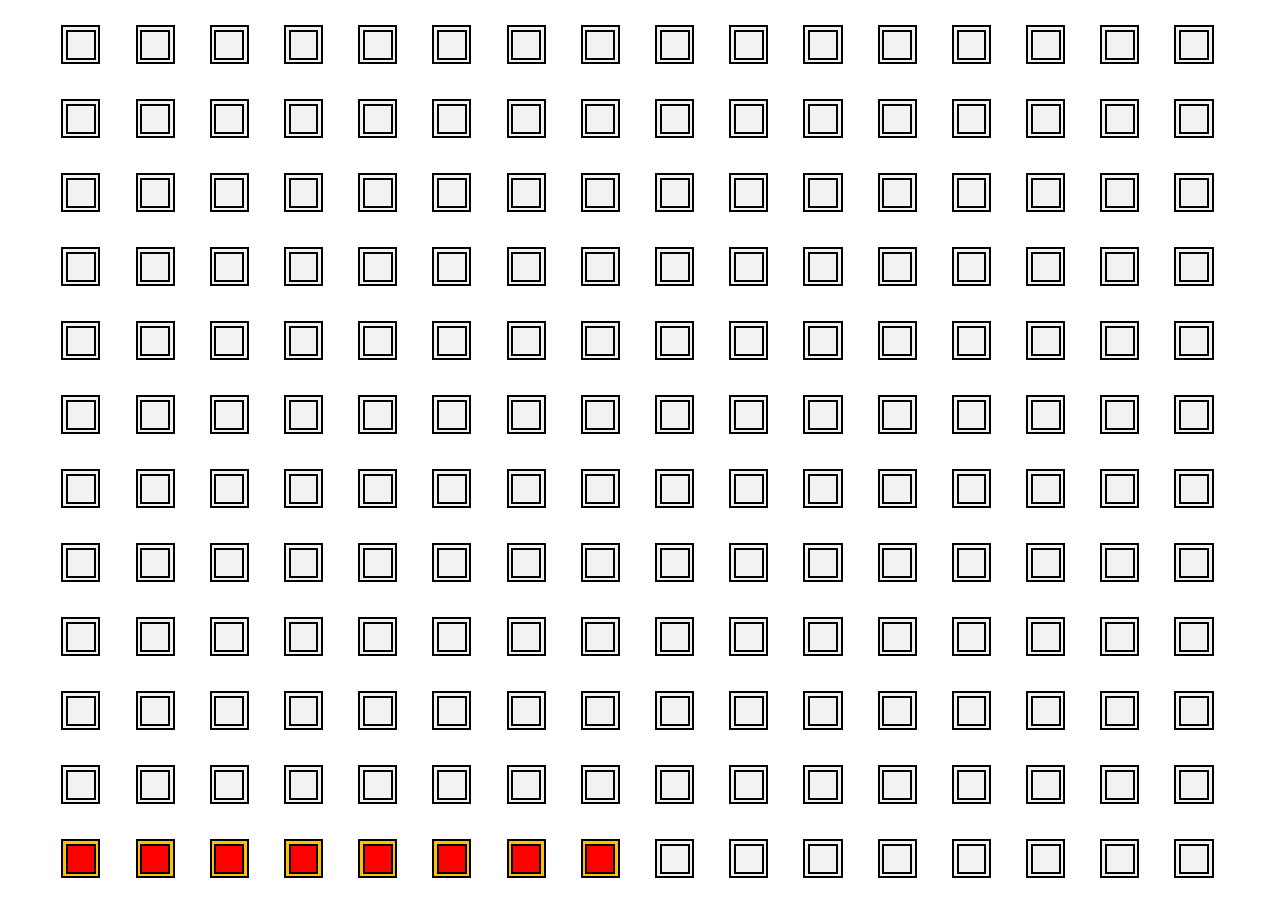
\includegraphics[width=0.35\linewidth]{figs/fig4.8.pdf}
    \caption{Серые элементы антенной решетки отключены во время оценки угла прихода на CSI-RS}
    \label{fig:4.8}
\end{figure}

\subsection{Оценка мощности}

Поскольку разрабатываемые алгоритмы должны быть основаны на мощности, ключевым
моментом является способ измерения мощности сигнала. Для каждой пары лучей UE-BS
у нас есть набор пилотных поднесущих, поэтому есть два пути измерения:
\begin{enumerate}
    \item Усреднить мощность по всем пилотным поднесущим.
    \item Использовать Фурье преобразование по всем пилотным поднесущим, перейти от частотной характеристики канала к временной и оценить мощность как максимум импульсной характеристиках канала.
\end{enumerate}

Возьмем для начала однолучевую модель канала. В этом случае сигнал, принятый на $q$-ой пилотной поднесущей примет вид
\begin{equation}
    x_q = a e^{-i2\pi q\Delta f \tau} + \xi_q,
\end{equation}
где $a$ комплексная амплитуда луча, включающая в себя диаграмму направленность
элемента, $\Delta f$ расстояние между пилотными поднесущими в частотной области,
$\tau$ -- задержка распространения, $\xi$ -- комплексны белый гауссовый шум с
мощностью $\sigma^2$.
Для первого варианта, оцененная мощность примет вид
\begin{equation}
    \hat p_1 = \frac{1}{Q} \sum\limits_{q = 0}^{Q - 1} \abs{x_q}^2,
\end{equation}
где $Q$ -- число пилотных поднесущих. После несложных вычислений, можем получить
\begin{equation}
    \mean{\hat p_1} = \abs{a}^2 + \sigma^2.
\end{equation}
\begin{equation}
    D_1 = \mean{p_1^2} - \mean{p_1}^2 = \frac{1}{Q}\qty(2\abs{a}^2 \sigma^2 + \sigma^4),
\end{equation}
где $\mean{\dots}$ -- математическое ожидание, $D$ -- дисперсия оценки мощности.



Во всех алгоритмах нас интересует $\abs{a}^2$ или пропорциональная ей величина.
Относительная систематическая ошибка $\delta_{s1}$ и относительная случайная ошибка $\delta_{r1}$ равны
\begin{equation}
    \delta_{s1} = \frac{\mean{\hat p_1} - \abs{a}^2}{\abs{a}^2} = \frac{\sigma^2}{\abs{a}^2},
\end{equation}
\begin{equation}
    \delta_{r1} = \frac{\sqrt{D_1}}{\abs{a}^2} =
    \frac{1}{\sqrt{Q}} \sqrt{2 \frac{\sigma^2}{\abs{2}} +
        \frac{\sigma^4}{\abs{a}^4}},
\end{equation}
Для второго варианта, оцененная мощность будет вычисляться следующим образом
\begin{equation}
    \hat p^2 = \max_n\qty(\frac{1}{Q} \sum\limits_{q=0}^{Q-1} x_q e^{-2 \pi q n /Q})^2,
\end{equation}
где $n$ -- индекс в оцененной дискретной ИХ канала. 
Если предположить, что выбор максимума всегда осуществляется корректно, можно
получить следующее
\begin{equation}
    \mean{\hat p_2} = \abs{a}^2 F + \frac{1}{Q}\sigma^2.
\end{equation}
\begin{equation}
    D_2 = \mean{\hat p_2^2} - \mean{\hat p_2}^2 = \frac{2\abs{a}^2 F \sigma^2}{Q},
\end{equation}
\begin{equation}
    F = \max_n \frac{\sin^2[\pi Q (\Delta f \tau - n/Q)]}{Q^2 \sin^2[\pi(\Delta f \tau - n/Q)]},
\end{equation}
\begin{equation}
    \frac{4}{\pi^2} \leq \frac{1}{Q^2 \sin^2[\frac{\pi}{2Q}]} \leq F \leq 1,
\end{equation}


Относительную систематическую ошибку $\delta_{s2}$ и относительную случайную ошибку $\delta_{r2}$ следует
определять как
\begin{equation}
    \delta_{s2} = \frac{\mean{\hat p_2} - F \abs{a}^2}{F \abs{a}^2} = \frac{1}{Q} \frac{\sigma^2}{F\abs{a}^2},
\end{equation}
\begin{equation}
    \delta_{r2} = \frac{\sqrt{D_1}}{F\abs{a}^2} = \frac{1}{\sqrt Q} \sqrt{\frac{2\sigma^2}{F\abs{a}^2}}.
\end{equation}
Второй подход лучше применять к оценке мощности для моноимпульса (см. \ref{sec:monopulse}) и случаев с
низкими ОСШ. Также, если задачей является оценка направления на основной луч в
многолучевом канале, второй подход уменьшает помехи, вызванными остальными лучами.
Однако в случае многолучевой оценки угла прихода второй подход приводит к
большой сложности, из-за необходимости рассматривать трехмерную задачу для
каждого возможного пути распространения.

Таким образом, в работе применяется следующая схема оценки мощности
\begin{enumerate}
    \item Для оценки угловой координаты в многолучевом канале, используется
    первый подход (усреднение принятой мощности по пилотным поднесущим). 
    \item Для оценки угловой координаты в однолучевом канале, применяется второй
    подход (Time Of Arrival selection). 
\end{enumerate}



\subsection[Иерархический поиск]{Иерархический поиск -- \baseline{}}
\label{sec:hSearch}\label{sec:hierarchy:search}
Эффективность иерархического поиска, в результатах симуляции в разделе
\ref{sec:simulations} он назван \textit{baseline}, рассматривается как нижняя
граница разработанных алгоритмов.  Можно было бы в качестве базового алгоритма
рассматривать метод Фурье (см. \ref{sec:Fourier}) и необходимый для него полный
перебор по всем парам лучей (UE-BS), примененный к меняющемуся во времени
каналу.  Однако он дает слишком высокую ошибку дискретизации и сравнивать и
редко применяется в реальных системах.

Алгоритм состоит из двух этапов: полного перебора всех пар лучей UE-BS и
процедуры дополнительных измерений.
На первом этапе пользователь использует ортогональную кодовую книгу, покрывающую
диапазон углов от $-\pi$ до $\pi$:
\begin{equation}
    \label{eq:4.16}
    \vec w_u =
    \begin{bmatrix}
        1 & \exp {i \eta_u} & \dots & \exp{i(N-1)\eta_u}
    \end{bmatrix}^T,
\end{equation}
\begin{equation}
    \label{eq:4.17}
    \eta_u = -\pi \frac{N-1}{N} + 2\pi \frac{u-1}{N},
\end{equation}
где $N$ -- число элементов антенной решетки, $u$ -- индекс весового вектора, лежащий в интервале $\qty[1 \dots N]$, $\eta_u$ -- обобщенный угол, соответствующий углу прихода сигнала следующим образом
\begin{equation}
    \eta_u = 2\pi \frac{d}{\lambda_w}\sin\phi_u,
\end{equation}
где $d$ -- расстояние между элементами решетки, $\lambda_w$ -- длина волны. ДН,
получаемые с помощью данной кодовой книги показаны на рис. \ref{fig:4.9}
сплошными линиями.
\begin{figure}[ht]
    \centering
    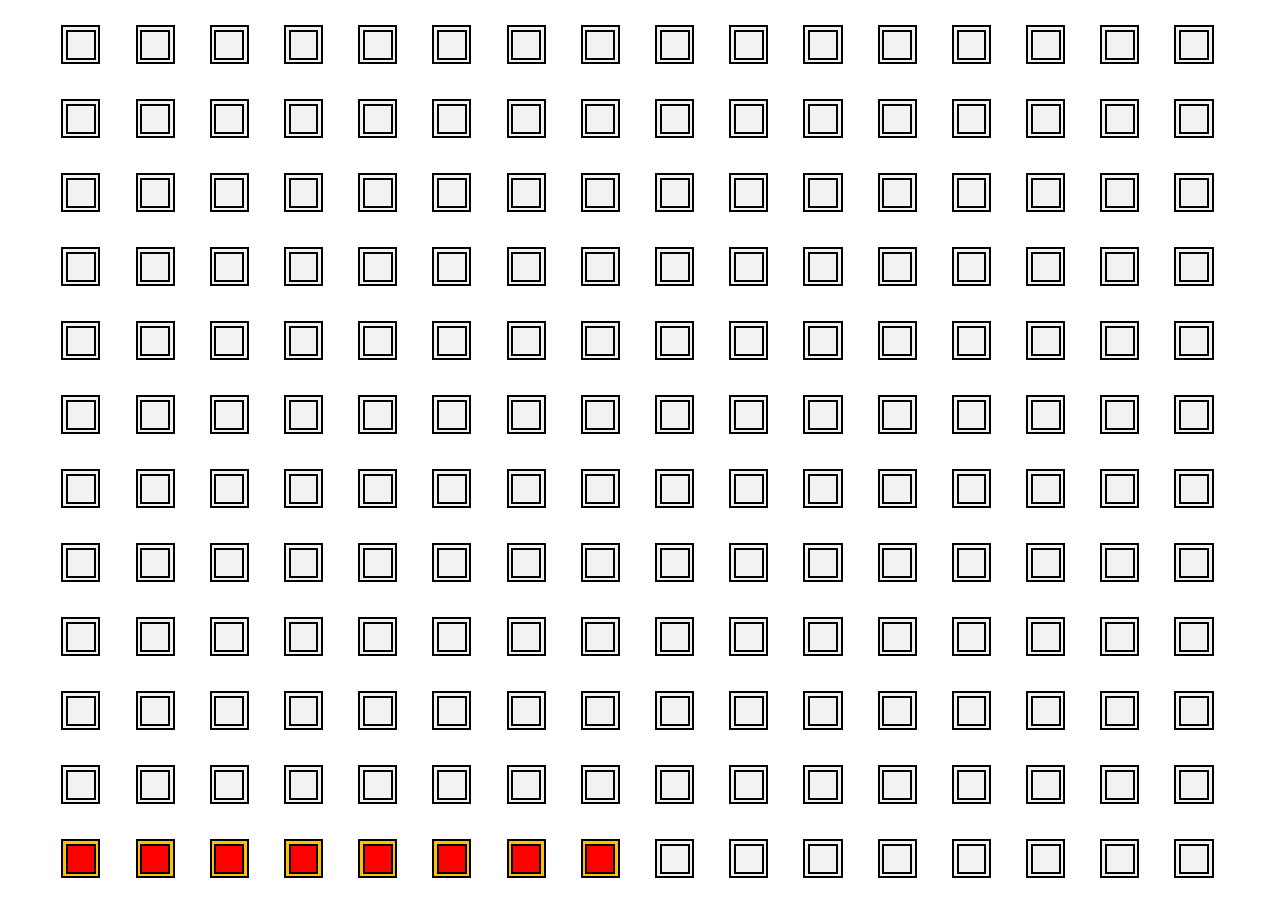
\includegraphics[width=0.5\linewidth]{figs/fig4.8.png}
    \caption{Различные ДН, формируемые кодовой книгой на стороне пользователя. $\psi$ -- обобщенный угол, $N=8$, $M=4$}
    \label{fig:4.9}
\end{figure}

Пусть $v$ -- индекс наилучшего весового вектора $\vec w_u^{(v)}$, который
обеспечивает наибольшую принятую мощность на антенной решетке.  Соответствующая
ДН показана на рис. \ref{fig:4.9} толстой сплошной линией. Пусть $p_v$ --
мощность, измеренная для вектора $\vec w_u^{(v)}$. На этапе дополнительных измерений
пользователь тестирует $M$ дополнительных весовых векторов, чтобы уменьшить
ошибку дискретизации.
\begin{equation}
    \label{eq:4.19}
    \vec w_q =
    \begin{bmatrix}
        1 & \exp {i \chi_q} & \dots & \exp{i(N-1)\chi_q}
    \end{bmatrix}^T,
\end{equation}
\begin{equation}
    \label{eq:4.20}
    \chi_q = \eta_v + 2\pi \frac{q}{N(M+1)},
\end{equation}
где $q=-0.5M,\dots,-1,+1,\dots,+0.5M$. Сформированные дополнительные ДН показаны
на рис. \ref{fig:4.9} пунктирными линиями.  Обозначим $p_0= p_v$ и $\chi_0 =
\eta_v$. Отметим, что для процедуры уточнения не нужно проводить измерения
$\chi_0$, поскольку оно уже было сделано на предыдущем этапе.  Наконец, путь
распространения с обобщенным углом $\hat \psi$ оценивается как один из $\chi_q
\in \qty{\chi_{-0.5 M}, \dots, \chi_0, \dots, \chi_{+0.5M}}$, обеспечивающий
наибольшую измеренную мощность $p_q$. Угол прихода соответствующего луча
оценивается как
\begin{equation}
    \label{eq:4.21}
    \hat \phi = \arcsin{\frac{\psi \lambda_w}{2\pi d}}.
\end{equation}

Процедура измерения алгоритма представлена на рис. \ref{fig:4.10} и происходит следующим образом:

\begin{enumerate}[label=\textbf{Шаг \arabic*:}]
    \item Этап сканирования по грубой сетке углов (Sector Level Sweep Stage). 
          BS периодически переключает свои лучи. 
          UE последовательно использует каждый луч из кодовой книги \eqref{eq:4.16} 
          и измеряет мощность на каждом луче BS.
    \item Выбирается пара лучей UE-BS с наибольшей измеренной мощностью.
          Обозначим направление лучшего луча пользователя обобщенным углом $\eta_v$.
    \item Процедура уточнения (дополнительных измерений). BS периодически переключает лучи. UE
          Пользователь последовательно использует лучи из кодовой книги \eqref{eq:4.19} 
          и измеряет мощность на каждой паре лучей UE-BS.
    \item Выбирается лучшая пара лучей UE-BS среди всех измеренных на шаге 3 и шаге 1. 
    Пусть выбранный луч UE имеет пространственную частоту $\hat \psi$.
    \item Если пара лучей UE-BS соответствовала AIP1, то $\hat \phi_{AOA} = \hat \phi$, где 
    $\hat \phi$ вычисляется из \eqref{eq:4.21}.
    Если выбранная пара лучей соответствовала AIP2, то $\hat \phi_{AOA} = \hat \phi + \pi$. 
\end{enumerate}

\begin{figure}[ht]
    \centering
    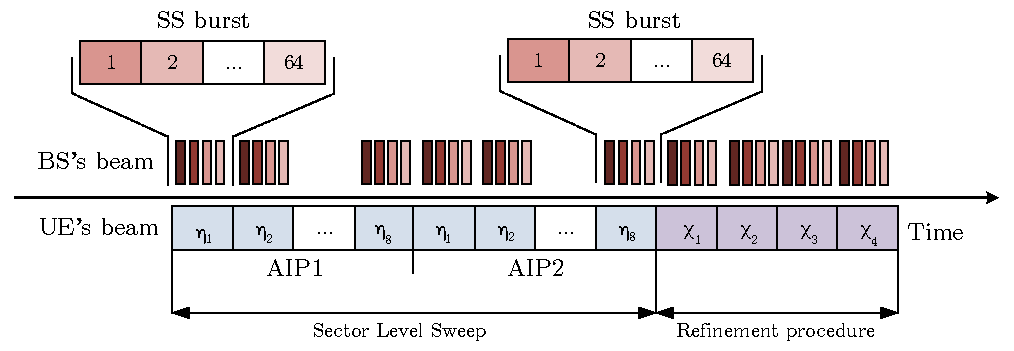
\includegraphics[width=\linewidth]{figs/fig4.9}
    \caption{Изображение процедуры иерархического поиска (\textit{baseline}) во времени для двух антенных решеток. $N=8$, $M=4$, 64 луча BS}
    \label{fig:4.10}
\end{figure}

Параметры алгоритма иерархического поиска представлены в таблице \ref{tab:4.2}, а его временн\'{а}я
структура на рис. \ref{fig:4.10}.
Предполагается, что один SS-burst состоит из 64 RS и занимает 32 последовательных слота с периодом 20 мс.
Для CSI-RS считаем, что период следования равен 4 слотам (0.5 мс) и могут быть
прозвонены два луча на двух разных цифровых портах.

\begin{table}
    \centering
    \caption{Параметры алгоритма иерархического поиска}
    \label{tab:4.2}
    \begin{tabular}{lcc}
        \toprule
        \midrule
        Структура RS                         & SS-burst  & CSI-RS    \\
        N / M / AIPs                         & 8 / 4 / 2 & 8 / 4 / 2 \\
        Число просканированных лучей (UE/BS) & 20 / 64   & 20/8      \\
        Суммарное число RS                   & 1280      & 160       \\
        Необходимое время                    & 384 мс    & 40 мс     \\
        \bottomrule
    \end{tabular}
\end{table}



\subsection[Иерархический поиск с минимизацией СКО]{Иерархический поиск с минимизацией СКО -- \hSearchMMSE{}}
\label{sec:hSearchMMSE:singlepath}
В теории оценивания AOA доказано, что наилучшее решение дает максимально правдоподобная оценка (Maximum Likelihood Estimator).
Рассматривая случай однолучевого канала, можно представить уравнение \eqref{eq:3.10} в виде
\begin{equation}
    d(\phi) = \sum\limits_q \vec y^H(q) \vec y(q) - \sum\limits_q\abs{\vec y^H \vec s(\phi)}^2 \to \min_\phi,
\end{equation}
\begin{equation}
    \label{eq:4.23}
    \sum\limits_q \abs{\vec y^H(q) \vec s(\phi)}^2 = \hat p(\phi) \to \max_\phi,
\end{equation}
где $\vec y$ -- вектор принятого антенной решеткой сигнала, $\vec s(\phi)$ --
фазирующий вектор. Выражение \eqref{eq:4.23} имеет смысл мощности,
принимаемой с  вектором $\vec s(\phi)$, обеспечивающим максимум ДН в направлении
$\phi$. Максимизация этого значения есть не что иное, как непрерывное
сканирование лучом и получение пространственного распределения мощности.

На практике, мы не можем применить этот оптимальный алгоритм по нескольким
причинам. Во-первых, мы  можем оценить только дискретный спектр мощности.
Разумеется, можно применить некоторые методы интерполяции, но это будет только
приближение.  Во-вторых, у нас есть сильные ограничения по времени, особенно в
случае динамического канала.  Таким образом, метод иерархического поиска,
который адаптивно измеряет дискретный спектр мощности, представляется наиболее
подходящей аппроксимацией оптимального МП-оценки.

Однако приближение спектра мощности с помощью иерархического
поиска, каким он рассматривался в предыдущем разделе \eqref{sec:hSearch}, не
является удачной аппроксимацией.  Прежде всего потому что это приближение с
ошибкой дискретизации. К тому же, если искомая угловая координата источника
лежит на стыке  двух антенных решеток $\hat \phi \approx \pm \pi/2$ или же просто
при низком ОСШ,  можно ошибиться с выбором антенной решетки и эта ошибка не
будет исправлена в дальнейшем. С учетом этим недостатков, был разработан
улучшенный алгоритм иерархического поиска.

На первый взгляд, проблема дискретизации может быть решена с помощью
МП-оценки, адаптированного к последовательному измерению отклика мощности
луча. Однако полученная в этом случае функция правдоподобия сложна для анализа
(здесь предполагается, что амплитуда принимаемого сигнала имеет распределение
Райса).

\begin{equation}
    F_{ML}(\psi, a) = \prod\limits_m \frac{1}{\sigma^2}
    \exp{-\frac{\hat p_m + a f_m(\psi)}{\sigma^2}
        I_0\qty(\frac{2\sqrt{\hat p_m a f_m(\psi)}}{\sigma^2})} \to \max_{\psi, a},
\end{equation}
где $\hat p_m$ -- измеренная мощность на $m$-ом луче, $\sigma^2$ -- мощность
шума, $a$ -- <<мощность>> некоторого пути распространения, $I_0(x)$ --
модифицированная функция Бесселя, $f_m(\psi)$ -- усиление АР для $m$-го луча в
направлении обобщенного угла $\chi_m$, $\psi = 2\pi \frac{d}{\lambda_w}\sin
    \phi$ -- обобщенный угол, а $\phi$ -- угол прихода.
\begin{equation}
    f_m(\psi) = \frac{\sin^2 (0.5N(\psi - \chi_m))}{\sin^2(0.5(\psi - \chi_m))}.
\end{equation}
Поскольку мы пытаемся найти простое решение, мы предлагаем взять в основу
критерий минимума СКО, вместо МП-оценки.
\begin{equation}
    \label{eq:26}
    F_{MMSE}(\psi, a) = \sum\limits_m \qty(\hat p_m - a f_m(\psi))^2 \to \min_{\psi,a}
\end{equation}
В первую очередь, необходимо исключить параметр $a$ из уравнения \eqref{eq:26}.
\begin{equation}
    \pdv{a} F_{MMSE}(\psi, a) = \sum\limits_m 2f_m(\psi) (\hat p_m - a f_m(\psi)) = 0
\end{equation}
\begin{equation}
    a(\psi) = \qty[\sum\limits_m f_m(\psi) \hat p_m][\sum\limits_m f_m^2(\psi)]^{-1}.
\end{equation}
Тогда, окончательный результат
\begin{equation}
    F_{MMSE}(\psi)=\underbrace{\sum\limits_m \hat p_m^2}_{\const} - \qty[\sum\limits_m f_m(\psi) \hat p_m]^2 \qty[\sum \limits_m f_m^2 (\psi)]^{-1} \to \max_{\psi}
\end{equation}
\begin{equation}
    \label{eq:4.30}
    F(\psi)=\qty[\sum\limits_m f_m(\psi) \hat p_m]^2 \qty[\sum \limits_m f_m^2 (\psi)]^{-1} \to \max_{\psi}
\end{equation}
На рис. \ref{fig:4.100} представлен вид функции \eqref{eq:4.30} во время процедуры уточнения для точной оценки угла прихода.

\begin{figure}[h!]
    \begin{subfigure}{0.49\linewidth}
        \centering
        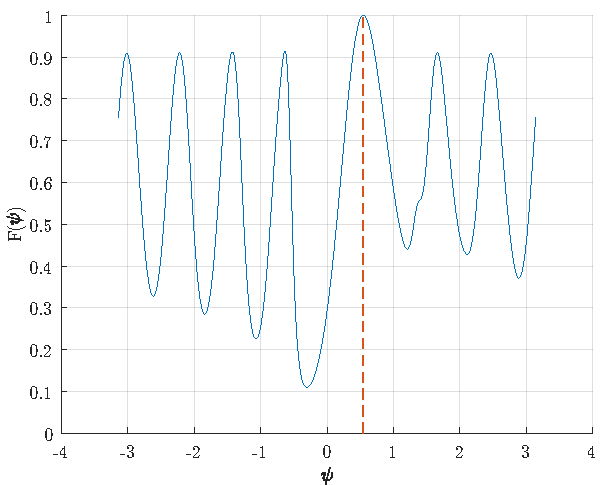
\includegraphics[width=\linewidth]{figs/fig4.10a}
        \caption{}
        \label{fig:4.10a}
    \end{subfigure}
    \begin{subfigure}{0.49\linewidth}
        \centering
        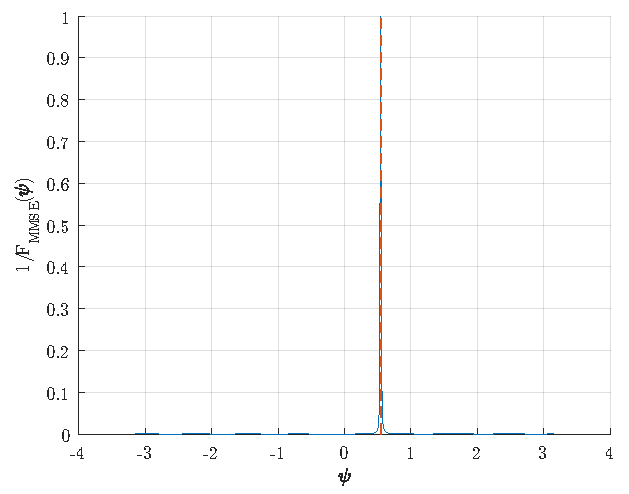
\includegraphics[width=\linewidth]{figs/fig4.10b}
        \caption{}
        \label{fig:4.10b}
    \end{subfigure}
    \caption{ (\subref{fig:4.10a}) Инверсная нормированная $F_{MMSE}(\psi)$,
    (\subref{fig:4.10b}) нормированная $F(\psi)$, $\psi=10^\circ(\psi \approx
    0.55), \text{SNR}=30$ дБ}
    \label{fig:4.100}
\end{figure}

Прямое вычисление $F(\psi)$ и поиск его максимума ведет к большим вычислительным затратам. Можно применить условие $F'(\psi) =0$ и получить следующее условие
\begin{equation}
    \label{eq:4.31}
    \begin{aligned}
        \mu(\psi) = &
        \qty(\sum\limits_m f'_m(\psi) \hat p_m) \qty(\sum\limits_m f^2_m(\psi))                              \\
                    & - \qty(\sum\limits_m f_m(\psi)\hat p_m) \qty(\sum\limits_m f_m (\psi) f'_m(\psi)) = 0,
    \end{aligned}
\end{equation}
\begin{equation}
    \label{eq:4.32}
    \begin{aligned}
        f'_m(\psi) = \frac{\sin(0.5N (\psi - \chi_m))}{2\sin^3(0.5(\psi - \chi_m))} \times
        \big[
          & (N-1)\sin(0.5(N+1) (\psi - \chi_m)) - \\
        - & (N+1) \sin(0.5(N-1)(\psi - \chi_m))
            \big]
    \end{aligned}
\end{equation}
Типичный график $\mu(\psi)$ представлен на рис. \ref{fig:4.12}. Можно заметить, что вокруг заданного $\psi \approx 0.55$ (красная вертикальная линия) есть область где
$\mu(\psi)$ положительна слева и отрицательна справа. Поэтому, если известна грубая оценка угла прихода,
что и происходит на первом этапе алгоритма,
можно методом дихотомии быстро найти AOA с машинной точностью.
\begin{figure}[h!]
    \centering
    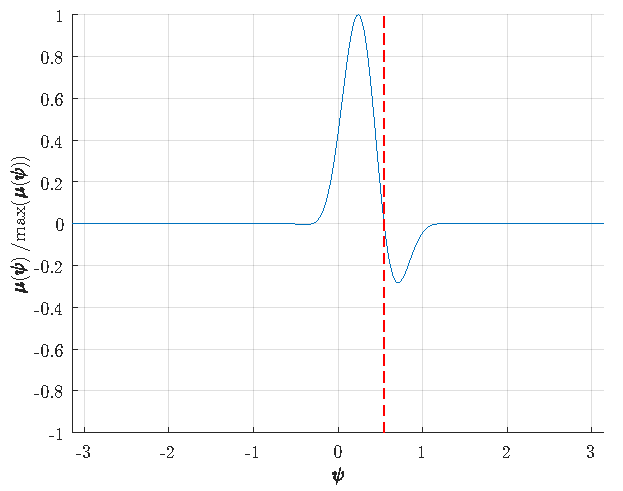
\includegraphics[width=0.5\linewidth]{figs/fig4.11}
    \caption{Нормированная функции $\mu(\psi)$, $\psi=10^{\circ} (\psi \approx 0.55), SNR=30$ дБ}
    \label{fig:4.12}
\end{figure}

\begin{algorithm}
    \caption{Метод дихотомии для оценки угла прихода для улучшенного алгоритма иерархического поиска (hSearchMMSE)}
    \label{lst:4.1}
    \begin{algorithmic}
        \State $\psi_{left} = \psi_{min}$
        \State $\psi_{right} = \psi_{max}$
        \State $\psi_{old} = \psi_{min}$
        \State $\Delta \psi = \infty$
        \While{$\Delta \psi > \epsilon$}
        \State $\hat \psi = 0.5 (\psi_{left} + \psi_{right})$
        \If{$\mu(\psi) < 0$}
        \State $\psi_{right} = \hat\psi$
        \Else
        \State $\psi_{left} = \hat\psi$
        \EndIf
        \State $\Delta \psi = \abs{\hat \psi - \psi_{old}}$
        \EndWhile
        \State \Return $0.5(\psi_{left} + \psi_{right})$
    \end{algorithmic}
\end{algorithm}

Заметим, что лучи вокруг фактического направления АОА вносят основной вклад в
\eqref{eq:4.30}, потому что они имеют более высокие веса. Таким образом, мы
можем рассматривать только лучи, измеренные на этапе процедуры уточнения, и
лучший луч, выбранный на этапе перебора по грубой сетке (Sector Level Sweep). Кроме того, для
процедуры поиска желательно, чтобы фактический угол прихода находился в середине
рассматриваемых направлений лучей. Таким образом, мы должны модифицировать
процедуру измерения на этапе дополнительных измерений. Примеры
представлены на рис.  \ref{fig:4.120}.
Сплошными серыми линиями показаны ДН лучей, формируемые на первом этапе оценки
(SLS). Сплошная красная линия -- ДН лучшего луча,
выбранного на первой стадии. Штриховые линии — ДН лучей на этапе
уточнения. Наконец, лучи, используемые в \eqref{eq:4.31}, отмечены цветными кривыми.

Всего, мы имеем два случая. В первом случае фактический угол прихода лежит
вблизи лучшего луча и мы проводим дополнительные измерения вокруг этого луча.
Во втором случае фактический угол прихода лежит посередине между лучшим и соседним
лучами. Следовательно, нам необходимо провести дополнительные измерения между ними.
В этом случае весовые векторы  формируются с помощью выражений \eqref{eq:4.19} и \eqref{eq:4.33}.
Знак в \eqref{eq:4.30} зависит от положения лучшего соседнего луча (слева или справа).
\begin{figure}[h!]
    \centering
    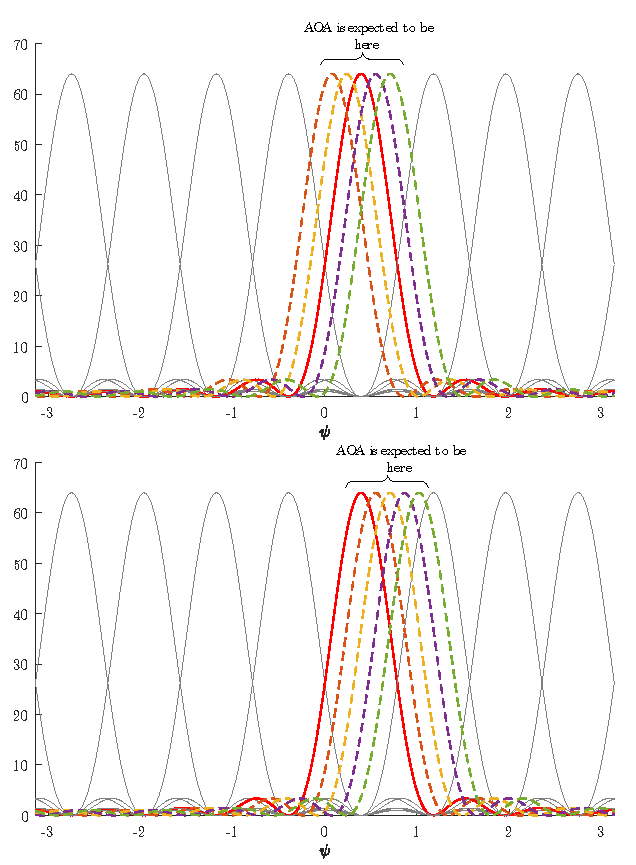
\includegraphics{figs/fig4.12}
    \caption{}
    \label{fig:4.120}
\end{figure}

\begin{equation}
    \label{eq:4.33}
    \chi_q = \eta_v \pm 2\pi \frac{q}{N(M+1)}; ~ q = 1 \dots M.
\end{equation}


Вопрос в том, как мы можем определить, где находится фактический угол прихода до этапа дополнительных измерений.
Предлагается использовать метрику \eqref{eq:4.30} для проверки трех гипотез:
\begin{itemize}
    \item $H_1$ -- угол прихода находится между лучшим лучом и левым соседним лучом
    \item $H_2$ -- угол прихода находится вблизи лучшего луча
    \item $H_3$ -- угол прихода находится между лучшим лучом и правым соседним лучом
\end{itemize}

\begin{figure}[h!]
    \centering
    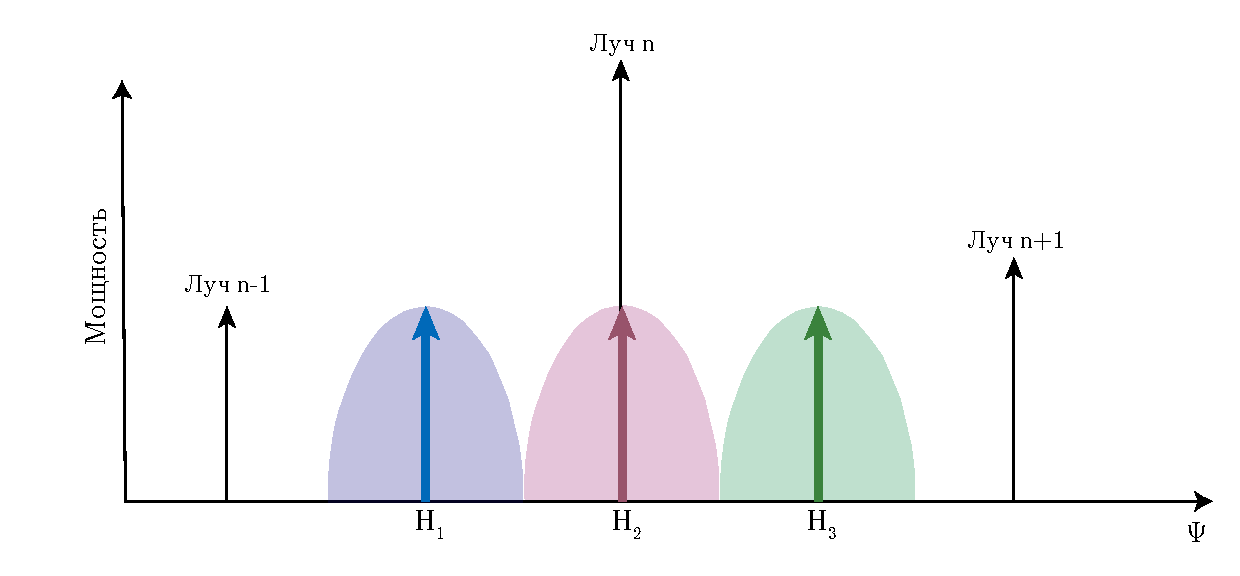
\includegraphics[width=0.75\linewidth]{figs/fig4.13}
    \caption{Выбор гипотез перед дополнительными измерениями. Черные стрелки принадлежат лучам из первой стадии прозвонки, цветные стрелки показывают центральные направления для различных гипотез}
    \label{fig:4.13}
\end{figure}

Если $\eta_v$ --  пространственная частота наилучшего луча на этапе основных измерений, выбранная нами метрика будет равна
\begin{equation}
    \label{eq:4.34}
    F_{H_n} = \qty[\sum\limits_{m=v-1}^{v+1} f_m (\psi_{H_n}) \hat p_m]^2 \qty[\sum\limits_{m=v-1}^{v+1}f_m^2(\psi_{H_n})]^{-1}
\end{equation}
\begin{equation}
    \label{eq:4.35}
    f_m(\psi_{H_n}) = \frac{\sin^2 (0.5N(\psi_{H_n} - \eta_{m}))}{\sin^2(0.5(\psi_{H_n} - \eta_{m}))}.
\end{equation}
\begin{equation}
    \label{eq:4.36}
    \begin{matrix}
        \psi_{H_1} = \frac{\eta_{v-1} + \eta_v}{2}; &
        \psi_{H_2} = \eta_{v}                       &
        \psi_{H_1} = \frac{\eta_{v+1} + \eta_v}{2}; &
    \end{matrix}
\end{equation}


Тогда структурная схема алгоритма будет следующей
\begin{enumerate}[label=\textbf{Шаг \arabic*:}]
    \item Этап полного перебора по грубой сетке (SLS). BS производит сканирование лучом, UE
          последовательно использует все лучи из своей кодовой книги \eqref{eq:4.16} для
          измерения мощности на каждом луче BS. Процедура выполняется для обоих АР.
    \item Выбирается лучшая пара лучей UE-BS и рассматривается выбранный луч UE
          как лучший сектор с пространственной частотой $\eta_v$.
    \item Проверяются гипотезы $H_1, H_2$ и $H_3$ (см. \ref{fig:4.13}) используя метрику \eqref{eq:4.34}.
          Выбирается гипотеза с наибольшим значением метрики. Отметим, что если в
          качестве лучшего луча выбирается первый луч UE ($v=1$), то гипотеза
          $H_1$ не тестируется.
          Аналогично, не тестируется гипотеза $H_3$ для последнего луча с
          индексом $v=8$.  \item  Этап дополнительных измерений. BS также
          производит сканирование лучом.  UE последовательно использует все лучи
          из кодовой книги \eqref{eq:4.19} для измерения мощности на каждом луче
          BS. Если выбрана гипотеза $H_2$, для формирования кодовой книги
          используется \eqref{eq:4.20}.  В остальных случаях используется
          \eqref{eq:4.33}. Знак <<$-$>> соответствует $H_1$, а <<$+$>>
          соответствует  $H_3$.
    \item Выполняется алгоритм поиска Алг. \ref{lst:4.1}, используя условие МСКО
          \eqref{eq:4.31}. В уравнение подставляется мощность лучшего луча, измеренная
          на шаге 2 и мощность лучей из шага 4. Луч BS выбирается таким же, как в
          лучшей паре на шаге 2.
    \item Рассчитывается угол прихода $\hat \phi$ на основе предполагаемой
          пространственной частоты. Если лучшая пара лучей UE-BS относится к АР\#1, то
          $\hat \phi_{AOA} = \hat \phi$. Если лучшая пара UE-BS относится к AР\#2, то
          $\hat \phi_{AOA} = \hat \phi + \pi$.
\end{enumerate}


Временн\'{а}я структура алгоритма иерархического поиска с минимизацией
среднеквадратичной ошибки (\textit{hSearchMMSE}) совпадает с \baseline{} и представлена на рис. \ref{fig:4.9}.
Параметры алгоритма представлены в табл. \ref{tab:4.3}.
\begin{table}
    \centering
    \caption{Параметры алгоритма hSearchMMSE}
    \label{tab:4.3}
    \begin{tabular}{lcc}
        \toprule
        \midrule
        Структура RS                                  & SS-burst  & CSI-RS    \\
        N / M / AIPs                                  & 8 / 4 / 2 & 8 / 2 / 2 \\
        Число просканированных \newline лучей (UE/BS) & 20 / 64   & 18 / 8    \\
        Суммарное число RS                            & 1280      & 144       \\
        Необходимое время (слот 0.125 мс)             & 384 мс    & 36 мс     \\
        \bottomrule
    \end{tabular}
\end{table}

\subsection[Модифицированный алгоритм моноимпульса]{Модифицированный алгоритм моноимпульса -- \AuxBeam{}}
\label{sec:AuxBeam:singlepath}
Идея алгоритма основанного на моноимпульсе, также известного как \textit{Auxiliary Beam}, была
предложена в \cite{Zhu2016} и \cite{Kim2019}. В отличие от обычных алгоритмов
моноимпульса (см. раздел \ref{sec:monopulse}), \AuxBeam{} основан на мощности и не
требует сложного измерения комплексной амплитуды. Кроме того, для зондирования требуется
достаточно малое количество лучей, и он совместим с алгоритмами слежения.

Основная идея в следующем. Пусть $\eta_u$ и $\eta_{u+1}$ -- обобщенные углы
лучей такие, что $\eta_u<\psi<\eta_{u+1}$ (см. рис. \ref{fig:4.14}), где $\psi$
-- обобщенный угол прихода волны.  Пусть $\eta_{u+1}$ ортогонален $\eta_u$, то
есть $\eta_{u+1} = \eta_u + 2\delta$, где $\delta = \pi/N$  и $\tilde \eta_u =
    0.5 (\eta_u + \eta_{u+1})$ -- центральное направление.
\begin{figure}[h!]
    \centering
    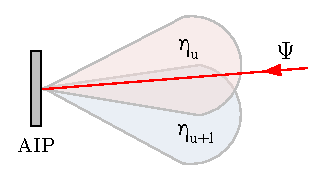
\includegraphics[width=0.5\linewidth]{figs/fig4.14}
    \caption{Конфигурация лучей для \AuxBeam{}}
    \label{fig:4.14}
\end{figure}
Тогда можно рассмотреть следующую метрику, однозначно зависящую от угла прихода
\begin{equation}
    \label{eq:4.37}
    \zeta(\psi) = \frac{f_u(\psi) - f_{u+1}(\psi)}{f_u(\psi) + f_{u+1}(\psi)} = - \frac{\sin(\psi - \tilde \eta_u) \sin \delta}{1 - \cos(\psi - \tilde \eta_u) \cos \delta}
\end{equation}
\begin{equation}
    \label{eq:4.38}
    f_u(\psi) = \frac{\sin^2 (0.5 N (\psi - \eta_u))}{\sin^2(0.5 (\psi - \eta_u))}
\end{equation}
Зависимость метрики $\zeta(\psi)$  от обобщенного угла прихода представлена на
рис. \ref{fig:4.15}.
\begin{figure}[h!]
    \centering
    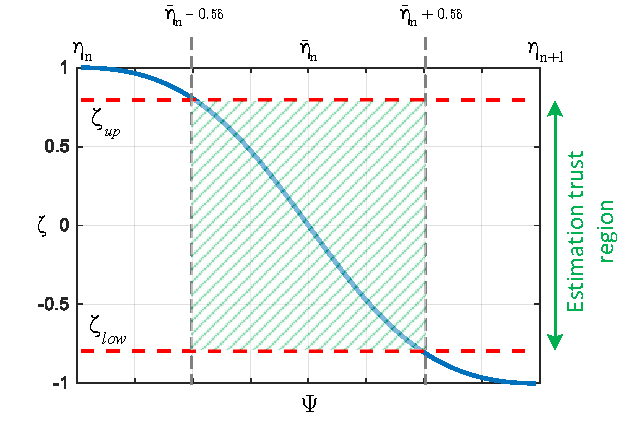
\includegraphics[width=0.5\linewidth]{figs/fig4.15}
    \caption{Зависимость метрики $\zeta(\psi)$ для алгоритма AuxBeam}
    \label{fig:4.15}
\end{figure}
В реальной системе метрика $\hat \zeta$ может быть оценена следующим образом
\begin{equation}
    \label{eq:4.39}
    \hat \zeta = \frac{\hat p_u - \hat p_{u+1}}{ \hat p_u + \hat p_{u+1} },
\end{equation}
где $\hat p_u$ -- мощность измеренная на $u$-ом луче. Эта оценка получается смещенной, поскольку $\hat p_u$ включает мощность шума.
Чтобы избежать этого, в знаменателе можно вычесть удвоенную мощность шума, но это может обратить метрику в бесконечность при малом SNR.
И, поскольку, функция $\zeta(\psi)$ достаточно полога на краях интервала $(\eta_u, \eta_{u+1})$, это приводит к высокому
воздействию шума на метрику при вычислении обратной функции.

Кроме того, если угол прихода находится рядом с центральным направлением определенного
луча, мы можем выбрать другой луч так, что условие $\eta_u<\psi < \eta_{u+1}$ не будет выполняться.
Чтобы этого не произошло, предлагается ввести условие на доверительный интервал
$\zeta_{low}<\hat \zeta < \zeta_{up}$, который изображен зеленой штриховкой  на рис.
\ref{fig:4.15}.

Если условие доверительного интервала не выполняется, следует провести дополнительные измерения на смещенных лучах.
Если оно выполняется, можно оценить угол прихода как
\begin{equation}
    \label{eq:4.41}
    \hat \psi = \tilde \eta_u - \arcsin(
    \frac{\hat \zeta \sin\delta}{\sin^2\delta + \hat \zeta^2 \cos^2\delta} -
    \frac{\hat \zeta \sqrt{1- \hat \zeta^2} \sin\delta\ \cos\delta}{\sin^2\delta + \hat \zeta^2 \cos^2\delta}
    )
\end{equation}
\begin{enumerate}[label=\textbf{Шаг \arabic*:}]
    \item Этап SLS. BS производит сканирование лучом, UE
          последовательно использует все лучи из кодовой книги \eqref{eq:4.16} для
          измерения мощности на каждом луче BS. Процедура выполняется для всех АР.
    \item По результатам измерений, выбирается лучшая пара лучей UE-BS. Для того же луча BS,
          выбирается самый сильный сосед, первого найденного луча. Используя измеренную мощность для выбранных лучей
          вычисляется метрика \eqref{eq:4.39}. Пример выбранных лучей UE представлен на рис. \ref{fig:4.17}.
    \item Если условие $\zeta_{low} < \hat \zeta < \zeta_{up}$, выполняется оценка обобщенного угла прихода $\hat \psi$ используя \eqref{eq:4.41} и пропускается шаг 4.
    \item Пусть $\eta_v$ -- обобщенный угол лучшего луча UE. Проводятся измерения на обобщенных углах
          $\eta_{v+0.5} = \eta_v - \delta$ и
          $\eta_{v-0.5} = \eta_v + \delta$. Дополнительные лучи показаны на рис. \ref{fig:4.17} пунктирными линиями. Далее вычисляется метрика \eqref{eq:4.39}
          и оценивается обобщенный угол прихода $\hat \psi$ (см. \eqref{eq:4.41}).
    \item Рассчитывается угол прихода $\hat \phi$ на основе предполагаемой пространственной частоты. Если лучшая пара лучей UE-BS
          относится к АР1, то $\hat \phi_{AOA} = \hat \phi$. Если лучшая пара UE-BS относится к АР2, то $\hat \phi_{AOA} = \hat \phi + \pi$.
\end{enumerate}

\begin{figure}[h!]
    \centering
    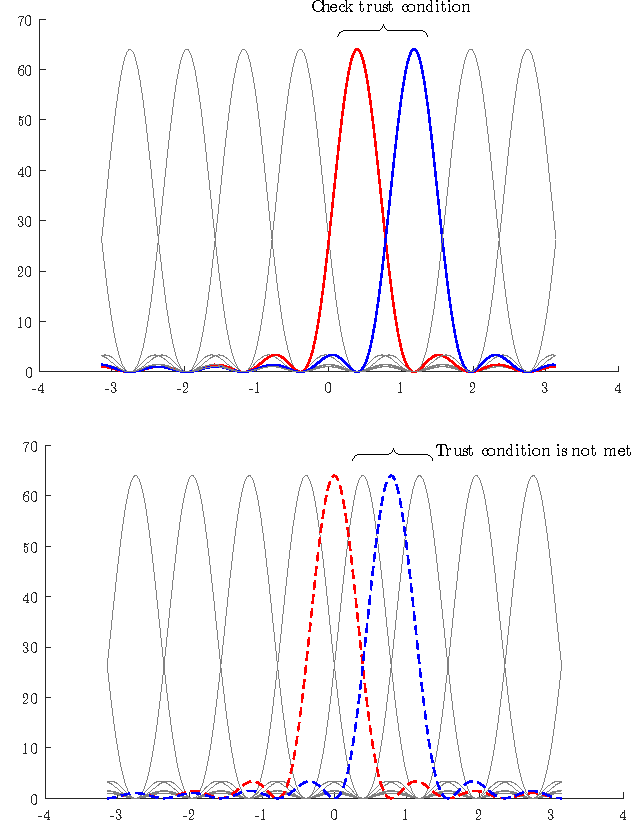
\includegraphics{figs/fig4.16}
    \caption{Два варианта выбора лучей UE для алгоритма AuxBeam. Верхний -- в случае выполнения условия на доверительный интервал, нижний -- в обратном случае.}
    \label{fig:4.17}
\end{figure}


\begin{figure}[h!]
    \centering
    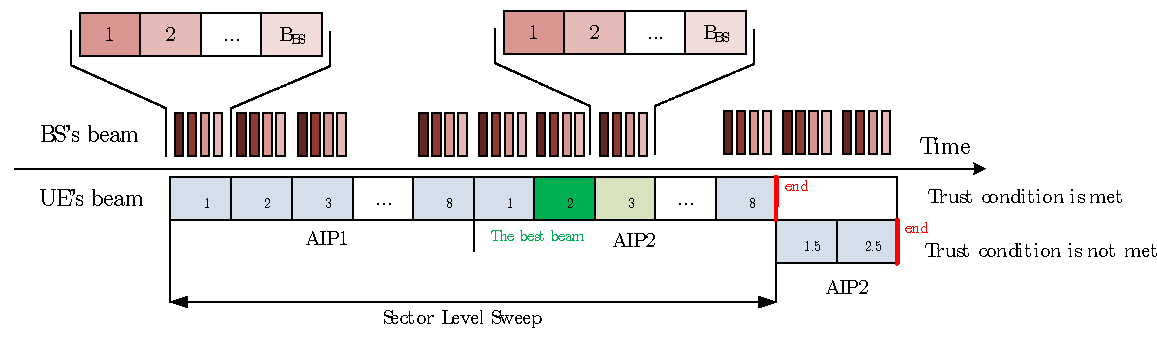
\includegraphics[width=\linewidth]{figs/fig4.17}
    \caption{Изображение \AuxBeam{} во времени для двух антенных решеток. $N=8$, $M=4$, 64 луча BS}
    \label{fig:timeline:auxbeam}
\end{figure}

Временн\'{а}я структура алгоритма AuxBeam представлена на рис. \ref{fig:timeline:auxbeam}. Параметры алгоритма представлены в табл. \ref{tab:parameters:auxbeam}.
\begin{table}
    \centering
    \caption{Параметры алгоритма AuxBeam}
    \label{tab:parameters:auxbeam}
    \begin{tabular}{lcc}
        \toprule
        \midrule
        Структура RS                         & SS burst        & CSI-RS        \\
        N / M / AIPs                         & 8 / 0 или 2 / 2 & 8 / 0 или 2/2 \\
        Число просканированных лучей (UE/BS) & 16 или 18 / 64  & 16 или 18 / 8 \\
        Суммарное число RS                   & 1024 или 1152   & 128 или 144   \\
        Необходимое время (слот 0.125 мс)    & 304 или 344 мс  & 32 или 36 мс  \\
        \hline
    \end{tabular}
\end{table}

\subsection[Сканирование адаптивным методом бисекций]{Сканирование адаптивным методом бисекций -- \ACS{}}
\label{sec:ACS:singlepath}

Еще один многообещающий метод —  Adaptive Compressed Sensing, идея которого описана \cite{Alkhateeb2014}.
Базовая концепция следующая. Пусть имеется сетка возможных
обобщенных углов прихода волны $\psi_q = - \pi\frac{(Q-1)}{Q} + \frac{2\pi}{Q} (q-1)$, где $Q$ -- размер сетки.
Мы можем представить сигнал, измеренный пользователем (UE) для фиксированного
луча BS, как
\begin{equation}
    \label{eq:4.42}
    y = \vec w^H\vec S \vec a + \vec \xi,
\end{equation}
\begin{equation}
    \label{eq:4.43}
    \vec S =
    \begin{bmatrix}
        \vec s(\psi_1) & \vec s(\psi_2) & \dots & \vec s(\psi_q) \\
    \end{bmatrix},
\end{equation}
\begin{equation}
    \label{eq:4.44}
    \vec s =
    \begin{bmatrix}
        1 & \exp{i\psi} & \dots & \exp\{ i(N-1)\psi\} \\
    \end{bmatrix}^T,
\end{equation}
\begin{equation}
    \label{eq:4.45}
    \vec a =
    \begin{bmatrix}
        0 & \dots & 0 & a & 0 & \dots 0 \\
    \end{bmatrix}^T,
\end{equation}

где $\vec w$ -- весовой вектор пользователя,
$\vec s(\psi)$ -- фазирующий вектор,
$N$ -- число элементов в антенной решетке,
$\vec \xi$ -- вектор шума,
$\vec z$ -- вектор комплексной амплитуды размерности $(Q\times 1)$,
где все элементы нулевые, кроме одного, отвечающему фактическому углу
прихода излучения на решетку.
Основная задача алгоритмов этого семейства -- восстановить вектор $\vec a$
используя количество измерений $L \ll Q$.  Если мы рассмотрим некоторую кодовую
книгу $\vec W$ размером $(N \times L)$, чьи столбцы являются весовыми векторами
для луча пользователя, результат сканирования будет
следующим
\begin{equation}
    \label{eq:4.46}
    y = \vec W^H\vec S \vec a + \vec \xi,
\end{equation}

В работе \cite{Alkhateeb2014}, авторы утверждают, что их адаптивный алгоритм более эффективен,
чем обычный алгоритм бисекций. В адаптивном алгоритме процедура зондирования разбита на несколько этапов
и кодовая книга $\vec W$ текущего этапа зависит от предыдущих результатов. Понятно, что если нас не интересует значение $a$, то
вектор $\vec a$ может быть сжат до вектора $\vec z$. Этот вектор кодирует позицию ненулевого элемента в векторе $\vec a$ (индекс $q$) и
требует только $\log(Q)$ итераций.

На первом шаге считаем, что ненулевой элемент имеет индекс от $1$ до $Q/2$ ($z_1=0$) или
$Q/2+1$ до $Q$ ($z_1=1$). Для этого нам необходимо сформировать кодовую книгу $\vec W$ размерности $(N \times 2)$, которая удовлетворяет условию
\begin{equation}
    \label{eq:4.47}
    \vec S^H \vec W = \alpha \vec G,
\end{equation}
\begin{equation}
    \label{eq:4.48}
    \vec G =
    \begin{pmatrix}
        1 & \dots & 1 & 0 & \dots & 0 \\
        0 & \dots & 0 & 1 & \dots & 1 \\
    \end{pmatrix}^T,
\end{equation}
где $\vec G$ -- матрица $(Q \times 2)$ и $\alpha$ -- нормировочный множитель.
Физически это означает, что первый весовой вектор должен обеспечивать однородную структуру ДН по
обобщенным углам $\psi_1 \dots \psi_{Q/2}$ и подавлять ДН в направлениях $\psi_{Q/2 + 1}\dots \psi_Q$. Второй весовой вектор должен обеспечивать противоположное распределение.
Приближенное решение для кодовой книги $\vec W$ получается следующим
\begin{equation}
    \label{eq:4.49}
    \vec W = \alpha (\vec S \vec S^H)^{-1} \vec S \vec G
\end{equation}

\begin{figure}[ht]
    \centering
    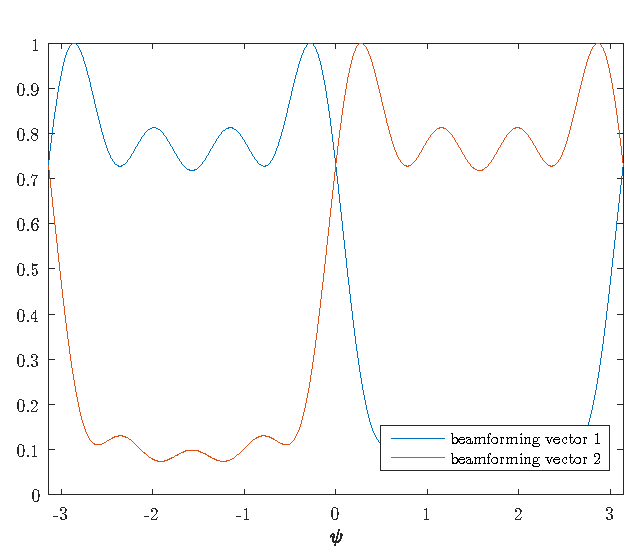
\includegraphics[width=0.5\linewidth]{figs/fig4.18}
    \caption{ДН для первого шага алгоритма $Q=40,~N=8$}
    \label{fig:4.18}
\end{figure}
Кодовый вектор, при котором будет принята наибольшая мощность будет соответствовать
первому приближению направления на источник. Пусть $z_1 = 0$. Тогда на следующим шаге
мы должны определить $z_2$. Это означает, что ненулевой элемент лежит между индексами $1$ или $Q/4$ ($z_2 =0 | z_1 =0$) или
между индексами $Q/4 + 1$ и $Q/2$ ($z_1 = 1 | z_1 = 0$). В этом случае матрица $\vec G$ определяется как
\begin{equation}
    \label{eq:4.50}
    \vec G =
    \begin{pmatrix}
        1 & \dots & 1 & 0 & \dots & 0 & 0 & \dots & 0 & 0 & \dots & 0 \\
        0 & \dots & 0 & 1 & \dots & 1 & 0 & \dots & 0 & 0 & \dots & 0 \\
    \end{pmatrix}^T.
\end{equation}
\begin{figure}[h!]
    \centering
    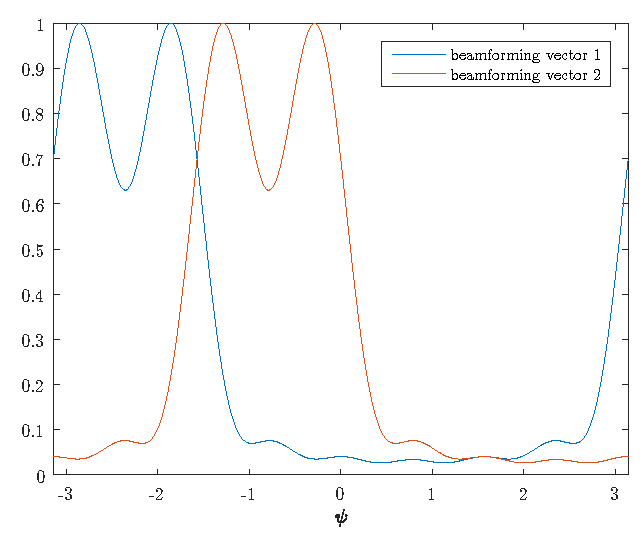
\includegraphics[width=0.5\linewidth]{figs/fig4.19}
    \caption{ДН для второго шага алгоритма, если $z_1=0$, $Q=40,~N=8$}
    \label{fig:4.19}
\end{figure}

Таким образом, ненулевые элементы в матрице $\vec G$ определяются сканированием необходимого индекса луча.
Процедура продолжается до тех пор, пока не будет определен последний элемент $z$. Проблема в том, что
с выбранной в данной работе аппаратной конфигурации пользователя мы не можем
применить \eqref{eq:4.49}, поскольку у нас не хватает степеней свободы, чтобы
обеспечить равномерное формирование направленности в одной области пространства
и полностью подавить другие. Поэтому, мы предлагаем некоторую модификацию этого алгоритма на основе дихотомии, следуя физическим принципам вышеизложенного.

\begin{enumerate}[label=\textbf{Шаг \arabic*:}]
    \item BS периодически переключает свои лучи, UE использует следующий весовой вектор $\vec w = \mqty*[1 & 0 & \dots & 0]^T$ для каждой AIP.
          Физически это означает, что отключаются все элементы АР, кроме одного. ДН всей решетки совпадает с ДН элемента и становится квазивсенаправленной.
          Выбирается та AIP, где результирующая измеренная мощность оказывается больше.
    \item BS периодически переключает свои лучи. Обозначим $\eta_{left} = - \pi$, $\eta_{right} = + \pi$.
          На стороне пользователя применяется следующая кодовая книга
          \begin{equation}
               \label{eq:4.51}
              \vec W =
              \begin{pmatrix}
                  \mqty{ 1 & \exp{i\eta_1}} & \zmat{1}{6} \\
                  \mqty{ 1 & \exp{i\eta_2}} & \zmat{1}{6} \\
              \end{pmatrix}
          \end{equation}
          \begin{equation}
              \eta_1 = \frac34 \eta_{left} + \frac14 \eta_{right}; ~ \eta_2 = \frac14 \eta_{left} + \frac34 \eta_{right}
          \end{equation}
          Если первый вектор бимформинга обеспечил наибольшую принятую мощность, то
          $\eta_{right} = 0.5 (\eta_{left} + \eta_{right})$.
          В другом случае
          $\eta_{left} = 0.5 (\eta_{left} + \eta_{right})$.
          
    \item BS периодически переключает свои лучи. Пользователь использует следующую кодовую книгу
          \begin{equation}
            \label{eq:4.53}
              \vec W =
              \begin{pmatrix}
                  \mqty{ 1 & \exp{i\eta_1} & \exp{i2\eta_1} & \exp{3i\eta_1}} & \zmat{1}{4} \\
                  \mqty{ 1 & \exp{i\eta_2} & \exp{i2\eta_2} & \exp{3i\eta_2}} & \zmat{1}{4} \\
              \end{pmatrix}
          \end{equation}
          \begin{equation}
              \eta_1 = \frac34 \eta_{left} + \frac14 \eta_{right}, ~ \eta_2 = \frac14 \eta_{left} + \frac34 \eta_{right}
          \end{equation}
          
          Если первый вектор бимформинга обеспечил наибольшую принятую мощность, то
          $\eta_{right} = 0.5 (\eta_{left} + \eta_{right})$.
          В другом случае
          $\eta_{left} = 0.5 (\eta_{left} + \eta_{right})$.
    \item BS периодически переключает свои лучи. Пользователь использует следующую кодовую книгу
          \begin{equation}
            \label{eq:4.55}
              \vec W =
              \begin{pmatrix}
                  1 & \exp{i\eta_1} & \exp{i2\eta_1} & \dots & \exp{i(N-1)\eta_1} \\
                  1 & \exp{i\eta_2} & \exp{i2\eta_2} & \dots & \exp{i(N-1)\eta_2}
              \end{pmatrix}
          \end{equation}
          \begin{equation}
              \eta_1 = \frac34 \eta_{left} + \frac14 \eta_{right}, ~ \eta_2 = \frac14 \eta_{left} + \frac34 \eta_{right}
          \end{equation}
          
          Если первый вектор бимформинга обеспечил наибольшую принятую мощность, то
          $\eta_{right} = 0.5 (\eta_{left} + \eta_{right})$.
          В другом случае
          $\eta_{left} = 0.5 (\eta_{left} + \eta_{right})$.
    \item Предыдущий шаг повторяется, пока не достигается желаемая точность. Отметим, что ширина ДН начиная с этого шага перестает меняться, изменяется только направление луча.
    \item Вычисляем угол прихода используя оцененный обобщенный угол $\hat \psi = 0.5 (\eta_{left} + \eta_{right})$. Если на шаге 1 была выбрана первая решетка, то
          $\hat \phi_{AOA} = \hat \phi$, в противном случае $\hat \phi_{AOA} = \hat \phi + \pi$.
\end{enumerate}
\begin{figure}[ht!]
\centering
\begin{subfigure}{0.49\linewidth}
    \centering
    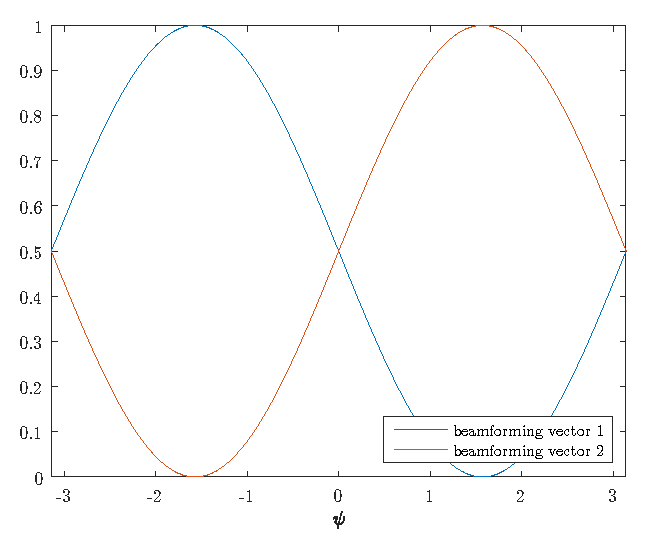
\includegraphics[width=\linewidth]{figs/fig4.20}
    \caption{}
    \label{fig:4.20}
\end{subfigure}
\begin{subfigure}{0.49\linewidth}
    \centering
    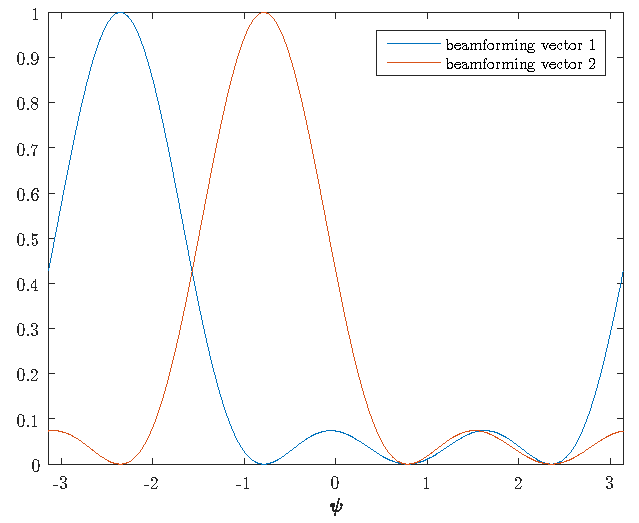
\includegraphics[width=\linewidth]{figs/fig4.21}
    \caption{}
    \label{fig:4.21}
\end{subfigure}
\begin{subfigure}{0.49\linewidth}
    \centering
    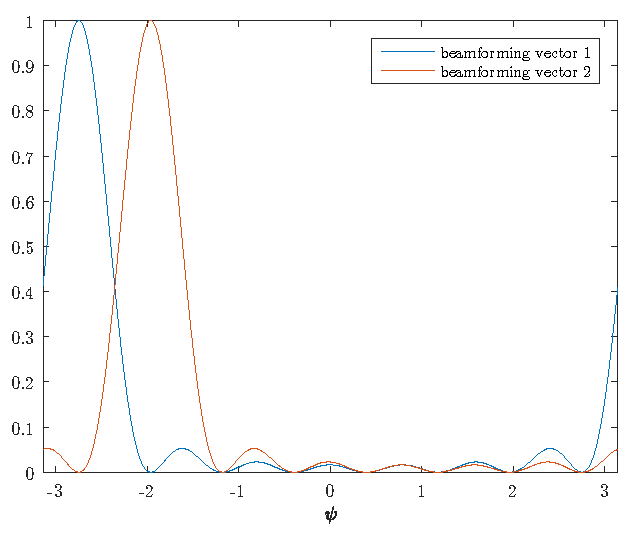
\includegraphics[width=\linewidth]{figs/fig4.22}
    \caption{}
    \label{fig:4.22}
\end{subfigure}
\caption{Диаграммы направленности, формируемые кодовыми книгами 
(\subref{fig:4.20}) -- \eqref{eq:4.51};
(\subref{fig:4.21}) -- \eqref{eq:4.53};
(\subref{fig:4.22}) -- \eqref{eq:4.55};
}
\label{fig:4.21-full}
\end{figure}

Временн\'{а}я структура метода бисекций (\textit{Compressed Sensing}) представлена на рис. \ref{fig:4.23}.
Параметры алгоритма представлены в табл. \ref{tab:4.5}.
\begin{table}[H]
    \centering
    \caption{Параметры метода бисекций}
    \label{tab:4.5}
    \begin{tabular}{lcc}
        \toprule
        \midrule
        Число уровней / Q (для одной АР)              & 8 / 128 & 8 / 128 \\
        Число просканированных \newline лучей (UE/BS) & 16 / 64 & 16 / 8  \\
        Суммарное число RS                            & 1024    & 128     \\
        Необходимое время (слот 0.125 мс)             & 304 мс  & 32 мс   \\
        \bottomrule
    \end{tabular}
\end{table}
\begin{figure}[H]
    \centering
    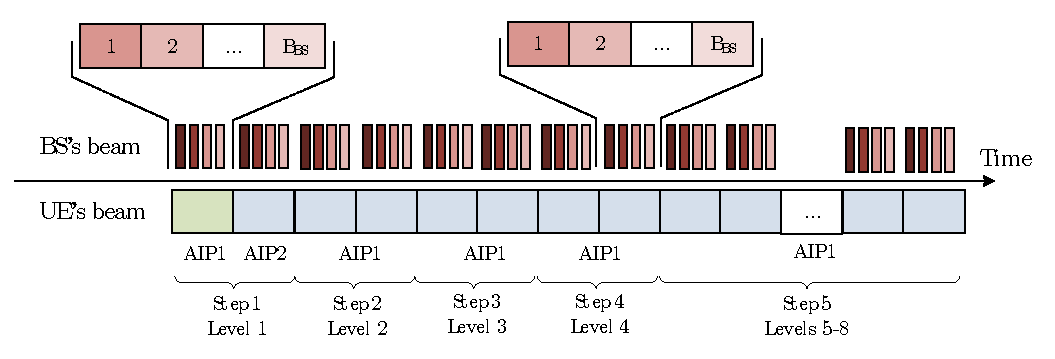
\includegraphics[width=\linewidth]{figs/fig4.23}
    \caption{Временная структура алгоритма \ACS{}}
    \label{fig:4.23}
\end{figure}

\section{Многолучевые алгоритмы оценки угла прихода сигнала}
\subsection{Иерархический поиск с минимизацией СКО}

Однолучевая версия алгоритма hSearchMMSE, описаная в разделе \ref{sec:4.4.2},
может быть расширина на многолучевую.  Однако, этот алгоритм есть аппроксимация
метода Фурье (непрерывного сканирования лучом), hSearchMMSE имеет характерные
недостатки.  Во-первых, разрешение ограничено шириной луча, но в контексте нашей
системы это не настолько критично. Второй недостаток более серьезный, он связан
с эффектов утечки мощности через боковые лепестки ДН.  Это означает, что мы
можем ошибочно распознать основной путь распространения, обнаруженный боковым
лепестком, как запасной путь.  Чтобы избежать подобной ошибки, необходимо
установить порог мощности для обнаружения запасного пути. Этот порог должен
учитывать утечку мощности через боковые лепестки и шумовое воздействие.

\begin{equation}
    \label{eq:4.57}
    Th_1^{mn} = A_n \frac{\sin^2(0.5 N (\eta_u - \hat \psi_1))}{\sin^2(0.5 (\eta_u - \hat \psi_1))} + 9 \sigma^2,
\end{equation}
\begin{equation}
    \label{eq:4.58}
    Th_2^{mn} = G A_n \frac{\sin^2(0.5 N (\eta_u - \hat \psi_1))}{\sin^2(0.5 (\eta_u - \hat \psi_1))} + 9 \sigma^2,
\end{equation}
где $n$ -- индекс луча базовой станции, $n$ -- индекс луча пользователя, $A_n$
-- <<мощность>> основного луча, включающая в себя ДН базовой станции, $G$ --
ослабление мощности элемента антенной решетки при приеме тыльной стороной
решетки ($-23$ дБ), $\eta_u$ -- направление луча пользователя в обобщенных
координатах, $\hat \psi_1$ -- оцененный угол прихода основного луча, $\sigma^2$
-- мощность шума, множитель $9$ добавлен исходя из правила $3\sigma$. Идея второго слагаемого в выражениях \eqref{eq:4.57},\eqref{eq:4.48} в том, чтобы 
уменьшить вероятность ложной тревоги из-за шума. Порог $Th_1$ используется для следящей решетки, той на которой был определен основой луч, а порог $Th_2$ для запасной решетки.
Величина $A_n$ может быть оценена, используя уравнение 
\begin{equation}
    A_n = \frac{1}{M+1} \sum\limits_{m=-M/2}^{M/2} \hat p_{mn} 
    \frac{\sin^2(0.5(\hat \psi_1 - \chi_m))}{0.5 N_{rx}(\hat \psi_1 - \chi_m)},
\end{equation}
где $\chi_m$ -- обобщенный угол, найденный на этапе сканирования (см. раздел \eqref{sec:4.4.2}), $\hat p_{mn}$ -- 
измеренная мощность на $m$-ом луче UE во время этапа дополнительных измерений и $n$-ом луче BS. Стоит отметить, что $A_n$ для каждого луча оченивается независимо. 

Пошагово алгоритм выглядит следующим образом. 
\begin{enumerate}[label=\textbf{Шаг \arabic*:}]
    \item BS производит сканирование лучом. UE последовательно использует
    каждый луч из кодовой книги \eqref{eq:4.16} для измерения мощности на каждом луче BS.
    Эта процедура выполняется для AIP1 и AIP2. Мощность измерения на этом этапе сохраняется в
    матрицах $\vec P_1$ и $\vec P_2$ соответственно. Каждый элемент матрицы соответствует
    определенным парам лучей UE и BS.
    \item Выбирается лучшая пара лучей UE-BS. Обозначим обобщенный угол лучшего луча как $\eta_{v1}$ и индекс лучшего луча BS как 
    $q_1$. 
    \item Тестируются гипотезы $H_1$, $H_2$, $H_3$ (см. рис. \ref{fig:4.14}) с помощью \eqref{eq:4.34}. Мощность на соседний лучах пользователя 
    ($u=v-1$, $u=v+1$) измеряется на одинаковых лучах BS с индексом $q_1$. Выбирается гипотеза с наибольшей метрикой \eqref{eq:4.34}.
    \item 
\end{enumerate}




<<<<<<< HEAD
\section{Результаты симуляций в модели канала Hotel Lobby}
=======
\section{Результаты симуляций в модели канала IEEE 802.11ay <<Hotel Lobby>>}
\label{sec:simulations}
Эффективность разработанных алгоритмов была исследована с помощью численного
моделирования. Использовалась реалистичная модель канала на основе трассировки
лучей, описанная в стандарте IEEE 802.11ay  \cite{Maltsev2017}. Сценарий
<<Hotel Lobby>> рассматривался как базовый сценарий.
Параметры симуляции представлены в табл. \ref{tab:4.3}.
По умолчанию максимальное количество переотражений в процедуре
трассировки лучей установлено равным 2.

Обычный сценарий Hotel Lobby предоставляет канал с лучом прямой видимости (LOS)
(см. рис. \ref{fig:4.30a}). Для того чтобы убрать луч прямой видимости (NLOS),
посередине комнаты была установлена дополнительная стена
(см. рис. \ref{fig:4.30b}).

\begin{figure}[ht]
  \centering
  \begin{subfigure}{0.49\linewidth}
    \centering
    \includegraphics[width=\linewidth]{figs/fig4.30a}
    \caption{}
    \label{fig:4.30a}
  \end{subfigure}
  \begin{subfigure}{0.49\linewidth}
    \centering
    \includegraphics[width=0.88\linewidth]{figs/fig4.30b}
    \caption{}
    \label{fig:4.30b}
  \end{subfigure}
  \caption{Схема расположения БС и пользователя в сценариях (\subref{fig:4.30a}) LOS
    и (\subref{fig:4.30b}) NLOS}
  \label{fig:4.30}
\end{figure}
\begin{figure}[H]
  \centering
  \begin{subfigure}{0.49\linewidth}
    \centering
    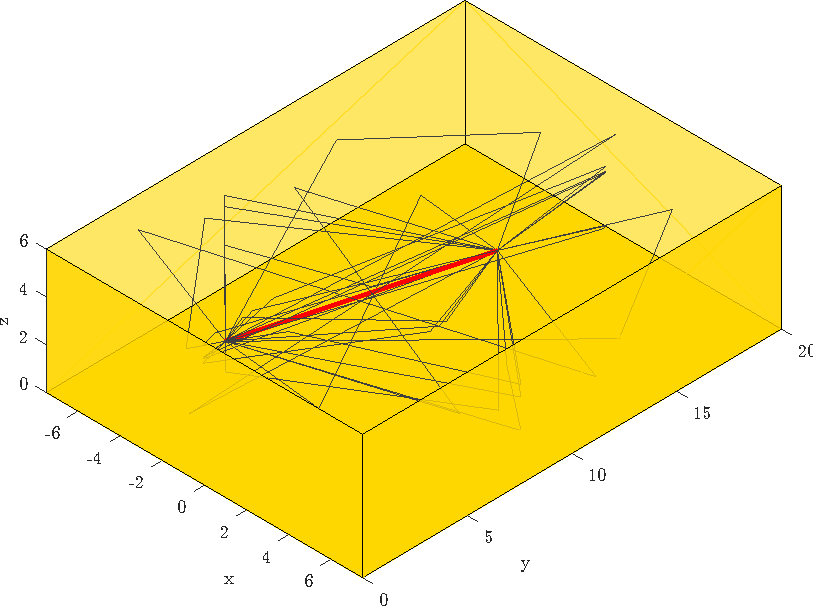
\includegraphics[width=\linewidth]{figs/4.30d.pdf}
    \caption{}
    \label{fig:4.30c}
  \end{subfigure}
  \begin{subfigure}{0.49\linewidth}
    \centering
    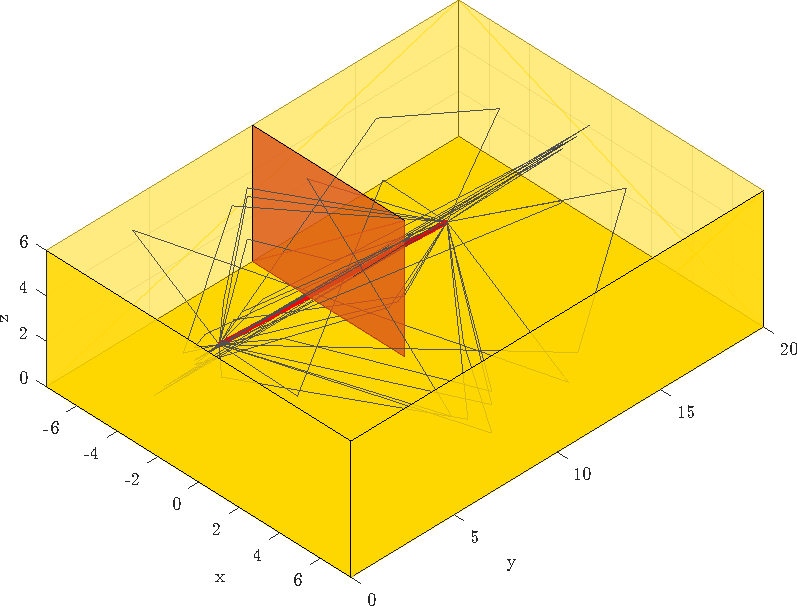
\includegraphics[width=\linewidth]{figs/4.30c.pdf}
    \caption{}
    \label{fig:4.30d}
  \end{subfigure}
  \caption{Геометрические лучи в сценариях (\subref{fig:4.30c}) LOS
    и (\subref{fig:4.30d}) NLOS. Красным цветом отмечен LOS-луч}
\end{figure}



В работе выполняется  Монте-Карло моделирование: пользователь вбрасывается
случайным образом в синих областях на рис. \ref{fig:4.30}.
Обе антенные решетки пользователя лежат в горизонтальной плоскости.
Азимут всех вброшенных пользователей также определялся случайным образом.
Количество независимых экспериментов составило 10000.

Были рассмотрены 4 различных сценария:
\begin{enumerate}
  \item Статичный LOS канал
  \item Статичный NLOS канал
  \item Быстро изменяющийся NLOS канал
  \item Случай низкого ОСШ
\end{enumerate}

В случае быстро меняющегося канала пользователи вращались в горизонтальной
плоскости с угловой скоростью 100 град/с. Дополнительное описание
сценария с низким ОСШ приведено в разделе \ref{sec:singlepath:static:LOW-SNR}.
Другие параметры моделирования и системы приведены в таблице \ref{tab:4.10}.

\begin{table}
  \centering
  \caption{Параметры системы}
  \label{tab:4.10}
  \begin{tabular}{ll}
    \toprule
    \textbf{Параметр}                   & \textbf{Значение}              \\
    \midrule
    Окружение                           & IEEE 802.11ay Hotel Lobby      \\
    Несущая частота                     & 28 ГГц (FR2)                   \\
    Ширина полосы                       & 50 МГц                         \\
    Частота дискретизации               & 61.44 МГц                      \\
    Размер БПФ                          & 512                            \\
    Число используемых поднесущих       & 384                            \\
    Число поднесущих в пилотном сигнале & 127 (SS burst) или 32 (CSI-RS) \\
    Расстояние между поднесущими        & 120 кГц                        \\
    Температура шума                    & 300 K                          \\
    Мощность шума на поднесущую         & -114 дБм                       \\
    \bottomrule
  \end{tabular}
\end{table}

Для оценки точности оцененного AOA, производилось его сравнение  с эффективным азимутальным углом
\eqref{eq:4.2} некоторого геометрического луча из модели.
В случае однолучевых алгоритмов  это в качестве этого луча выбирался самый сильный
путь распространения. В представленных результатах разница между оцененным AOA и эффективным азимутом
геометрического луча отмечается как <<error>>.
Для оценки точности многолучевых алгоритмов  выполнялась более сложная процедура.
Во-первых, сортировался список геометрических лучей в порядке убывания коэффициента передачи.
Далее удалялись те лучи, которые находились в пределах ширины ДН вокруг самого сильного из них.
После этого следующий в списке лучей рассматривался как самый сильный и процедура повторялась до
конца всего списка.

Обозначим $\phi_1$ и $\phi_2$ как оценку AOA для основного и запасного лучей соответственно.
Пусть $\Psi$ -- список геометрических AOA, а $\psi_1$ —
АОА сильнейшего геометрического луча.
Ошибка определения основного луча $\psi_1$ определялась как наименьшая величина
между $\abs{\phi_1 - \psi_1}$ и  $\abs{\phi_2 - \psi_1}$.
Пусть наименьшая ошибка определилась на угле $\phi_1$ .
Ошибка определения запасного луча   $\min(\Psi - \phi_2)$,
т.е. ближайший геометрический луч будет считаться опорным для
резервного луча.

В качестве показателей эффективности рассматривались
следующие метрики:

\newcommand\CDF{\text{CDF}}
\begin{itemize}
  \item Функция распределения ошибки (\CDF) оценки AOA
  \item Среднеквадратичная ошибка (СКО)
  \item Среднее значение ошибки ($\CDF = 0.5$)
  \item Значение $\CDF$ по уровню 0.8 и 0.9
\end{itemize}

Предполагается, что алгоритмы работают, если ошибка меньше удвоенной ширины
ДН ($25,2^{\circ}$).  СКО учитывает только эксперименты, в которых
алгоритмы работают успешно.
Вероятность отказа работы алгоритма также измерялась.

Однолучевые  разработанные алгоритмы сравнивались с базовым алгоритмом
иерархического поиска (см.  раздел \ref{sec:hSearch}).  В случае многолучевости
базовая линия отсутствует.

Во всех случаях оценивалось типичное значение ОСШ, которое определялось
как отношение мощности сигнала и шума на одну поднесущую при идеальном
формировании луча.

\pgfplotstableset{
  col sep=semicolon, % the seperator in our .csv file
  every head row/.style={%
      output empty row,
      before row={\toprule%
          Алгоритм
          &\multicolumn{2}{c}{СКО, град}
          & $P_{fail}$
          &\multicolumn{2}{c}{CDF = 0.9, град}
          &\multicolumn{2}{c}{CDF = 0.8, град}
          &\multicolumn{2}{c}{CDF = 0.5, град}
          \\\midrule},
    },
  every last row/.style={after row=\bottomrule},
  string type,
}
\subsection{Однолучевые алгоритмы: стат. случай в LOS}


\begin{figure}[ht]
  \centering
  \includegraphics{results/rus/singlepath-static-LOS-1}
  \caption{Функция распределения (CDF) ошибки определения угла прихода. Стат. случай, LOS}
  \label{fig:singlepath:static:LOS}
\end{figure}

В первую очередь, однолучевые алгоритмы были протестированы в статическом LOS сценарии.
В качестве пилотного сигнала был выбран SS-burst, мощность передатчика $-15$ дБм.
ОСШ на одну поднесущую было от 10 до 40 дБ в большинстве случаев.
Приблизительно в 2\% случаев, ОСШ находилось в интервале от -10 дБ до 10 дБ.

Результаты моделирования представлены на рис. \ref{fig:singlepath:static:LOS} и
табл. \ref{tab:singlepath:static:LOS}. 
\begin{table}[h!]
  \begin{center}
    \caption{Стат. случай, LOS}
    \small
    \label{tab:singlepath:static:LOS}
    \pgfplotstabletypeset{results/rus/singlepath-static-LOS.csv} % filename/path to file
  \end{center}
\end{table}

По результатам моделирования видно, что все разработанные алгоритмы показывают 
схожие результаты и все они луче базовой линии (их кривые CDF находятся всегда
левее базовой кривой). Наличие ошибок в данном случае вызвано эффектом
замираний, приводящего к флуктуациям восстанавливаемого AOA относительно LOS
направления.  Замирания возникают из-за того, что помимо основного LOS луча,
рядом находятся также лучи, отраженные от потолка, пола, стены рядом с БС и
другие с первым порядком отражения, мощность не сильно меньше, чем у LOS луча.
Все эти лучи имеют разный эффективный азимут \eqref{eq:4.2}, поэтому в некоторых
измерениях восстанавливается не направление на главный луч, а направление на
один из лучей главного кластера. Это приводит к высокому значению <<ошибки>>,
превышающей теоретическую, для всех алгоритмов.

Также можно заметить, что в 13\% экспериментов ошибка оценки AOA составляет
более $25.2^\circ$ для всех алгоритмов. Это связано с <<краевым эффектом>>,
когда угол прихода близок к значению $\pm 90^\circ$ (см. рис. \ref{fig:4.5}).
Во-первых, эти направления равноправны с точки зрения волнового фронта и их
нельзя различить с помощью АР.  Это приводит к некоторым случайным скачкам около
$180^\circ$. Эта проблема может частично решаться с помощью кодовой книги, где
ни один луч не имеет направлений на $\pm 90^\circ$.  Во-вторых, при таких
значениях AOA появляется неоднозначность выбора между АР пользователя и поэтому
выбор АР становится случайным. В результате на функции распределения появляется 
некоторая <<полка>> (см. рис. \ref{fig:singlepath:static:LOSa}), вызванная этими
двумя эффектами.
\begin{figure}[ht]
  \centering
  \includegraphics{results/rus/singlepath-static-LOS-full-1}
  \caption{Функция распределения (CDF) ошибки определения угла прихода. Стат. случай, LOS}
  \label{fig:singlepath:static:LOSa}
\end{figure}

\subsection{Однолучевые алгоритмы: стат. случай в NLOS}
\label{sec:singlepath:static:NLOS}

Также разработанные алгоритмы тестировались на статическом NLOS сценарии.
В качестве пилотного сигнала используется SS-burst, мощность передатчика равна -15 дБм.
ОСШ на поднесущую составляет от -5 до 20 дБ в большинстве случаев.
Приблизительно в 9\% случаев значение ОСШ находилось в диапазоне от -25 до -5 дБ.

Результаты моделирования представлены на рис. \ref{fig:singlepath:static:NLOS} и
табл. \ref{tab:singlepath:static:LOS}.  Иерархический поиск (\textit{baseline},
см. раздел \ref{sec:hSearch}) отмечен синим цветом, иерархический поиск с
минимизацией СКО (\textit{hSearchMMSE}, см. раздел
\ref{sec:hSearchMMSE:singlepath}) -- оранжевым, модифицированный алгоритм
моноимпульса (\textit{AuxBeam}, см. раздел \ref{sec:AuxBeam:singlepath}) --
красным цветом, адаптивный алгоритм бинарного поиска (\textit{ACS}, см. раздел
\ref{sec:ACS:singlepath}) -- фиолетовым.




\begin{figure}[ht]
  \centering
  \includegraphics{results/rus/singlepath-static-NLOS-1}
  \caption{Функция распределения (CDF) ошибки определения угла прихода. Стат. случай, NLOS}
  \label{fig:singlepath:static:NLOS}
\end{figure}
\begin{table}[h!]
  \begin{center}
    \caption{Стат. случай, NLOS}
    \small
    \label{tab:singlepath:static:NLOS}
    \pgfplotstabletypeset{results/rus/singlepath-static-NLOS.csv} % filename/path to file
  \end{center}
\end{table}

В данном сценарии, разброс главного кластера геометрических лучей меньше, чем в
LOS, поэтому точность определения AOA выше. Лучшим решением в данном случае
являются \textit{AuxBeam} и \textit{hSearchMMSE}, поскольку они не имеют ошибки
квантования. Их функции распределения и другие метрики практически одинаковы.
\textit{ACS}-алгоритм имеет конечную ошибку квантования
$\Delta \psi = 0.0246 (\Delta \phi \approx 0.5^\circ)$, что и наблюдается в
результатах.  Также отметим, что несмотря на относительное низкое ОСШ на одну
поднесущую, точность представленных алгоритмов достаточно высоки. Это происходит
из-за усреденения по 127 пилотным поднесущим в SS-burst.

\subsection{Однолучевые алгоритмы: быстро меняющийся канал}
\label{sec:singlepath:rotation:NLOS}
Интересным случаем является быстро меняющийся NLOS канал. Мощность передатчика
равна 23 дБм.  ОСШ на поднесущую в большинстве случаев составляет от 30 до 60
дБ. Примерно в 3\% случаев ОСШ находится в диапазоне от 10 до 30 дБ.

\begin{figure}[ht]
  \centering
  \includegraphics{results/rus/singlepath-rotation-NLOS-1}
  \caption{Функция распределения (CDF) ошибки определения угла прихода. Динам. случай, NLOS, SS-burst}
  \label{fig:singlepath:rotation:NLOS-1}
\end{figure}
Результаты симуляции представлены на рис. \ref{fig:singlepath:static:NLOS} и
табл.  \ref{tab:singlepath:static:NLOS}.
Для SS-burst с периодом 20 мс процедура сканирования для этого сценария слишком долгая --
от 300 до 380 мс, что соответствует углу поворота от 30 до 38 градусов (ширина ДН $12.6^\circ$).
Лучше всего работает \textit{ACS}-алгоритм, поскольку на начальных этапах
он использует широкую ДН, устойчивую к вращению пользователя. 

Остальные алгоритмы работают плохо, и ошибка оказывается равномерно
распределенной в пределах поворота пользователя за время измерения.  В среднем,
продолжительность \AuxBeam{} меньше, чем \hSearchMMSE{}, что дает
ему преимущество. Стоит отметить, что в 25 \% случаев ошибка \AuxBeam{}
менее 3 град. Это соответствует начальным условиям, когда фактический AOA
находится между двумя последними прозвоненными лучами и полученные измерения не успевают
устареть.

Эффективность \hSearchMMSE{} немного выше базового алгоритма, в силу 
его меньшей длительности: на этапе дополнительных измерений измерялись только 2 луча,
т.е. общее количество измеренных лучей равно 18, в то время как у \baseline{} --
20. Стоит отметить, что этап дополнительных измерений после процедуры SLS, работает по сильно 
устаревшим данным, что делает саму процедуру почти бесполезной. 

Гораздо лучшее решение предоставляется с помощью CSI-RS (см. рис.
\ref{fig:singlepath:rotation:NLOS-1} и табл. \ref{tab:singlepath:static:NLOS})в
качестве пилотных сигналов. Продолжительность прозвонки в этом случае составляет
от 32 до 40 мс, что соответствует повороту пользователя на 3.2 - 4.0 град.

В этом случае наилучшее решение дает алгоритм \AuxBeam, поскольку
его длительность одна из самых низких. 
\ACS алгоритм несмотря на такую же длительность работает значительно хуже, 
поскольку у него есть ошибка квантования.
\hSearchMMSE, несмотря на свою длительность, не имеют ошибки квантования и его 
эффективность во многих случаях совпадает с \AuxBeam{}.
\begin{table}[h!]
  \begin{center}
    \caption{Динам. случай, NLOS, SS-burst}
    \small
    \label{tab:singlepath:rotation:NLOS}
    \pgfplotstabletypeset{results/rus/singlepath-rotation-NLOS.csv} % filename/path to file
  \end{center}
\end{table}

\begin{figure}[ht]
  \centering
  \includegraphics{results/rus/singlepath-rotation-NLOS-CSI-RS-1}
  \caption{Функция распределения (CDF) ошибки определения угла прихода. Динам. случай, NLOS, CSI-RS}
  \label{fig:singlepath:rotation:NLOS-2}
\end{figure}

\begin{table}[h!]
  \begin{center}
    \caption{Динам. случай, NLOS, CSI-RS}
    \small
    \label{tab:singlepath:rotation:NLOS-2}
    \pgfplotstabletypeset{results/rus/singlepath-rotation-NLOS-2.csv} % filename/path to file
  \end{center}
\end{table}

\subsection{Однолучевые алгоритмы: низкое ОСШ}
\label{sec:singlepath:static:LOW-SNR}
Чтобы протестировать алгоритмы в сценарии с низким ОСШ, 
большинство лучей были заблокированы с помощью дополнительной стены так, чтобы
пользователь находился в отдельном помещении. 

В симуляции моделировались отражения до 4-го порядка.
В этом случае <<самый сильный>> луч входит в комнату
через <<дверь>> и достигает пользователя после четырехкратного отражения. Геометрия
представлена на рис. \ref{fig:4.36} (более слабые лучи тоже присутствуют в
симуляции, но они не изображены на рисунке).
Положение пользователя было зафиксировано. Ориентация пользователя в горизонтальной плоскости была
случайной.

\begin{figure}[ht]
  \centering
  \includegraphics[width=.5\linewidth]{figs/fig4.36}
  \caption{Геометрия симуляций для случая низкого ОСШ}
  \label{fig:4.36}
\end{figure}

Мощность передатчика равна -10 дБм. ОСШ на одну поднесущую находится в диапазоне
от -47 до -25 дБ. В качестве опорного сигнала выбран SS-burst. 

Результаты симуляции представлены на рис.\ref{fig:singlepath:static:LOW-SNR} и
табл.  \ref{tab:singlepath:static:LOW-SNR}.  Иерархический поиск (\baseline{},
см.  раздел \ref{sec:hSearch}) отмечен синим цветом, разработанный иерархический
поиск с минимизацией СКО (\hSearchMMSE{}, см. раздел
\ref{sec:hSearchMMSE:singlepath}) -- оранжевым $(M=2)$ и зеленым $(M=4)$,
модифицированный алгоритм моноимпульса (\AuxBeam{}, см. раздел
\ref{sec:AuxBeam:singlepath}) -- красным цветом, адаптивный алгоритм бинарного
поиска (\ACS{}, см. раздел \ref{sec:ACS:singlepath}) -- фиолетовым.
\begin{figure}[ht]
  \centering
  \includegraphics{results/rus/singlepath-static-LOW-SNR-1}
  \caption{Функция распределения (CDF) ошибки определения угла прихода. Стат. случай, LOS, основной луч}
  \label{fig:singlepath:static:LOW-SNR}
\end{figure}

\begin{table}[h!]
  \begin{center}
    \caption{Низкое ОСШ}
    \small
    \label{tab:singlepath:static:LOW-SNR}
    \pgfplotstabletypeset{results/rus/singlepath-static-LOW-SNR.csv} % filename/path to file
  \end{center}
\end{table}


Из результатов моделирования видно, все алгоритмы, кроме \ACS{}, работают хорошо в
68\% случаев. При этом практически все алгоритмы проигрывают \baseline{} в
значении СКО (кроме \AuxBeam{}). Наличие высоких ошибок оценки
АОА не позволяют дать точную оценку СКО для приемлемого количества
экспериментов. С точки зрения медианного значения ошибки $(CDF = 0,5)$
кажется более подходящей метрикой. Оба варианта \hSearchMMSE{} и \AuxBeam{}
превосходят базовый уровень по этому показателю.  Мы видим, что наилучшее
решение дает алгоритм \hSearchMMSE{} $(M = 4)$.  

Наихудшим решением в случае низкого ОСШ является \ACS{}. На самом деле, этот
алгоритм в данном случае не оценивает AOA, а лишь возвращает равномерно
распределенное случайное значение. Это вызвано тем, что \ACS{} на первых двух
итерациях использует широкие ДН, что приводит низкому усилению АР и высокой
вероятности ошибки в выборе начального сектора. 


\pgfplotstableset{
  fixed zerofill,
  col sep=semicolon, % the seperator in our .csv file
  string type,
  precision=2,
  every last row/.style={after row=\bottomrule},
  every head row/.style={
      before row={\toprule},
      after row={
          \midrule},
    }
}
\subsection{Многолучевые алгоритмы: стат. случай в LOS}

Многолучевые алгоритмы были протестированы в статическом LOS сценарии. В
качестве опорного сигнала использовался SS-burst.  Мощность передатчика была
установлена равной 10 дБм. ОСШ на поднесущую
составляло от 35 до 65 дБ в подавляющем большинстве случаев. Примерно в 3\%
случаев значение ОСШ находилось в диапазоне от 19 до 35 дБ.  

Полученные результаты моделирования и показатели эффективности для основного
луча представлены на рис. \ref{fig:multipath:static:LOS:1}  и табл.
\ref{fig:multipath:static:LOS:1}. Полученные результаты моделирования и
показатели эффективности запасного луча представлены на рис.
\ref{fig:multipath:static:LOS:2} и в табл. \ref{tab:multipath:static:LOS:2}.
\begin{figure}[H]
  \centering
  \includegraphics{results/rus/multipath-static-LOS-1}
  \caption{Функция распределения (CDF) ошибки определения угла прихода. Стат. случай, LOS, основной луч}
  \label{fig:multipath:static:LOS:1}
\end{figure}
\begin{table}[H]
  \begin{center}
    \caption{Стат. случай, LOS, основной луч}
    \label{tab:multipath:static:LOS:1}
    \pgfplotstabletypeset{results/rus/multipath-static-LOS-1.csv}
  \end{center}
\end{table}
Для оценки угла прихода основного луча \AuxBeam{}, \hSearchMMSE{} и \ACS{} показывают
почти одинаковую эффективность. Тот же результат
наблюдался и в случае однолучевых версий алгоритмов. 

Для резервного луча \hSearchMMSE{} в 10\% случаев не нашел луча или он был ассоциирован 
с основным лучом. Подобные случаи исключались из набора данных в CDF и таблицах.
Для \AuxBeam{} это значение составило 5\%, для \ACS{} -- 47\%. Такой плохой результат 
\ACS{} связан прежде всего с эффектом утечки мощности главного луча через 
боковые лепестки ДН. 

По результатам моделирования можно сделать вывод, что \AuxBeam{} и
\hSearchMMSE{} позволяют достаточно хорошо оценить направление на запасной луч.

\begin{figure}[H]
  \centering
  \includegraphics{results/rus/multipath-static-LOS-2}
  \caption{Функция распределения (CDF) ошибки определения угла прихода. Стат. случай, LOS, запасной луч}
  \label{fig:multipath:static:LOS:2}
\end{figure}
\begin{table}[H]
  \begin{center}
    \caption{Стат. случай, LOS, запасной луч}
    \label{tab:multipath:static:LOS:2}
    \pgfplotstabletypeset{results/rus/multipath-static-LOS-2.csv}
  \end{center}
\end{table}

\subsection{Многолучевые алгоритмы: стат. случай в NLOS }
\begin{figure}[H]
  \centering
  \includegraphics{results/rus/multipath-static-NLOS-1}
  \caption{Функция распределения (CDF) ошибки определения угла прихода. Стат. случай, NLOS, основной луч}
  \label{fig:multipath:static:NLOS:1}
\end{figure}

\begin{table}[H]
  \begin{center}
    \caption{Стат. случай, NLOS, основной луч}
    \label{tab:multipath:static:NLOS:1}
    \pgfplotstabletypeset{results/rus/multipath-static-NLOS-1.csv}
  \end{center}
\end{table}

\begin{table}[H]
  \begin{center}
    \caption{Стат. случай, NLOS, запасной луч}
    \label{tab:multipath:static:NLOS:2}
    \pgfplotstabletypeset{results/rus/multipath-static-NLOS-2.csv}
  \end{center}
\end{table}
\begin{figure}[H]
  \centering
  \includegraphics{results/rus/multipath-static-NLOS-2}
  \caption{Функция распределения (CDF) ошибки определения угла прихода. Стат. случай, NLOS, запасной луч}
  \label{fig:multipath:static:NLOS:2}
\end{figure}

\subsection{Многолучевые алгоритмы: быстро меняющийся канал}
Другим интересным сценарием является быстро меняющийся канал NLOS. Здесь были
приняты во внимание аналогичные результаты однолучевых алгоритмов (см. раздел
\ref{sec:singlepath:rotation:NLOS}) и использовался только CSI-RS.  Мощность
передатчика устанавливалась равным 23 дБм.  Отношение сигнал/шум на поднесущую в
подавляющем большинстве случаев составляло от 25 до 55 дБ.  Примерно в 3\%
случаев значение SNR находилось в диапазоне от 10 до 25 дБ.

Полученные результаты моделирования и показатели эффективности для основного луча представлены на
рис. \ref{fig:multipath:rotation:NLOS:1} и в табл. \ref{tab:multipath:rotation:NLOS:1}. 
Полученные результаты моделирования и показатели эффективности для резервного
луча представлены на рис. \ref{fig:multipath:rotation:NLOS:2} и в табл. \ref{tab:multipath:rotation:NLOS:2}.
\begin{figure}[H]
  \centering
  \includegraphics{results/rus/multipath-rotation-NLOS-1}
  \caption{Функция распределения (CDF) ошибки определения угла прихода. Динам. случай, NLOS, основной луч}
  \label{fig:multipath:rotation:NLOS:1}
\end{figure}

\begin{table}[H]
  \begin{center}
    \caption{Динам. случай, NLOS, основной луч}
    \label{tab:multipath:rotation:NLOS:1}
    \pgfplotstabletypeset{results/rus/multipath-rotation-NLOS-1.csv}
  \end{center}
\end{table}

\begin{figure}[H]
  \centering
  \includegraphics{results/rus/multipath-rotation-NLOS-2}
  \caption{Функция распределения (CDF) ошибки определения угла прихода. Динам. случай, NLOS, запасной луч}
  \label{fig:multipath:rotation:NLOS:2}
\end{figure}

\begin{table}[H]
  \begin{center}
    \caption{Динам. случай, NLOS, запасной луч}
    \label{tab:multipath:rotation:NLOS:2}
    \pgfplotstabletypeset{results/rus/multipath-rotation-NLOS-2.csv} % filename/path to file
  \end{center}
\end{table}


Длительность алгоритмов находится в диапазоне от 32 до 64 мс, что соответствует повороту на 3.2 - 6.4 град.
Мы снова видим, что наилучшее решение для основного луча дает кратчайший алгоритм, т.е.
\AuxBeam{} (требуется 32-40 мс). Второй результат показывает \hSearchMMSE{}, продолжительность которого составляет
40 мс (всегда прозванивается два дополнительных луча на этапе уточнения). 

Что касается резервного луча, то наибольшую эффективность обеспечивает \hSearchMMSE{} в силу своей короткой длительности 
и большей гибкости по сравнению с \AuxBeam{}.
\ACS{} не нашел резервный путь в 26\% всех случаев. Эти случаи
были исключены из набора данных для получения CDF и метрик. Для других алгоритмов эти значения были
менее 0.5\%.

\subsection{Многолучевые алгоритмы: низкое ОСШ}
Многолучевые алгоритмы были протестированы в статическом сценарии NLOS с низким
ОСШ. В качестве опорного сигнала был выбран SS-burst. 
Мощность передатчика была установлена равной -25
дБм. Отношение сигнал/шум на поднесущую составило от -30 до 5 дБ в
большинстве случаев. Примерно в 3\% случаев значение ОСШ находилось в
диапазоне от -80 до -30 дБ.

Полученные результаты моделирования для основного луча представлены на
рис.\ref{fig:multipath:static:LOW-SNR:1} и 
табл.\ref{tab:multipath:static:LOW-SNR:1}. Результаты моделирования для
резервного пути представлены на рис. \ref{fig:multipath:static:LOW-SNR:2} и табл.
\ref{tab:multipath:static:LOW-SNR:2}.

\begin{figure}[H]
  \centering
  \includegraphics{results/rus/multipath-static-LOW-SNR-1}
  \caption{Функция распределения (CDF) ошибки определения угла прихода. Низкое ОСШ, основной луч}
  \label{fig:multipath:static:LOW-SNR:1}
\end{figure}

\begin{table}[H]
  \begin{center}
    \caption{Низкое ОСШ, основной луч}
    \label{tab:multipath:static:LOW-SNR:1}
    \pgfplotstabletypeset{results/rus/multipath-static-NLOS-1.csv}
  \end{center}
\end{table}

\begin{figure}[H]
  \centering
  \includegraphics{results/rus/multipath-static-LOW-SNR-2}
  \caption{Функция распределения (CDF) ошибки определения угла прихода. Низкое ОСШ, запасной луч}
  \label{fig:multipath:static:LOW-SNR:2}
\end{figure}

\begin{table}[H]
  \begin{center}
    \caption{Низкое ОСШ, запасной луч}
    \label{tab:multipath:static:LOW-SNR:2}
    \pgfplotstabletypeset{results/rus/multipath-static-NLOS-2.csv} % filename/path to file
  \end{center}
\end{table}

Как и ожидалось, наилучшее решение дает алгоритм \hSearchMMSE{}, который
является аппроксимацией алгоритма Фурье и не имеет ошибки квантования. Что
касается других алгоритмов, \ACS{} не
нашел резервный путь в 53\% случаев, в то время как  для \AuxBeam{} и \hSearchMMSE{} 
это значение составило 1-3\%.  Эти случаи были исключены из набора
данных для получения CDF и таблиц. Также следует отметить, что \AuxBeam{}
более подвержен влиянию низкого ОСШ по сравнению с \hSearchMMSE{}. 
Это связано с нестабильностью метрики \eqref{eq:4.39}, особенно в случаях, когда 
сигнал подавляется ДН элементов АР, что ведет к чрезвычайно низкому ОСШ.
>>>>>>> main


%! TeX root = ../main.tex
\SafetyRules
При выполнении компьютерного моделирования на персональной
ЭВМ соблюдалась техника безопасности в
соответствии с СанПин 2.2.2/2.4.1340-03 \cite{SanPin}.  В помещениях для работы на
компьютерах необходимым условием является наличие естественного и искусственного
освещения.  Естественное освещение реализуется через окна, ориентированные
преимущественно на север и северо-восток. Не допускается размещение мест
пользователей ПЭВМ в цокольных и подвальных помещениях.  Искусственное освещение
должно осуществляться системой общего равномерного освещения. Яркость
светильников в зоне углов излучения от 50 до 90 градусов с вертикалью в
продольной и поперечной плоскостях должна составлять не более 200 кд/м$^2$,
защитный угол светильников должен быть не менее 40 градусов. В случае работы
преимущественно с документами, допускается применение комбинированного
освещения: кроме общего устанавливаются светильники местного освещения, которые
не должны создавать бликов на поверхности экрана и увеличивать его освещенность
более 300 лк.  Площадь одного рабочего места для взрослых пользователей должна
составлять не менее 6 м$^2$, а объем – не менее 20 м$^3$.  Для внутренней отделки
помещений должны использоваться диффузно-отражающие материалы с коэффициентом
отражения от потолка – $0.7–0.8$; для стен – $0.5–0.6$; для пола – $0.3–0.5$.
Поверхность пола в помещениях должна быть ровной, без выбоин, нескользкой,
удобной для очистки и влажной уборки, обладать антистатическими свойствами.
Микроклимат в помещениях, где установлены компьютеры, должен соответствовать
санитарным нормам: температура воздуха в теплый период года должна быть не более
23–25 градусов Цельсия, в холодный – 22–24 градуса Цельсия; относительная
влажность воздуха должна составлять 40–60; скорость движения воздуха – 0.1 м/с.

Для повышения влажности воздуха в помещениях следует применять увлажнители
воздуха, заправляемые ежедневно дистиллированной или прокипяченной питьевой
водой. Помещения перед началом и после окончания работы за компьютером следует
проветривать.  Экран видеомонитора должен находиться от глаз пользователя на
оптимальном расстоянии 600-700 мм, но не ближе 500 мм с учетом размеров
алфавитно-цифровых знаков и символов. При непрерывной работе с компьютером
каждые 1-2 часа делать перерыв на 10-15 минут для отдыха и выполнения комплекса
физкультурно-оздоровительных упражнений.



% \nocite{*}
\newpage
\printbibliography


\end{document}



% [1]M. Giordani, M. Polese, A. Roy, D. Castor and M. Zorzi, "A Tutorial on Beam Management for
% 3GPP NR at mmWave Frequencies," IEEE Communications Surveys & Tutorials, vol. 21, no. 1,
% pp. 173-196, 2019.
% [2]IEEE doc. 802.11-09/0334r8 Channel Models for 60 GHz WLAN Systems, A. Maltsev et al., May
% 2010.
% [3] IEEE doc. 802.11-15/1150r9 Channel Models for IEEE 802.11ay, A. Maltsev et al., March 2017.
% [4]H. Xu, V. Kukshya and T. S. Rappaport, “Spatial and temporal characteristics of 60-GHz indoor
% channels,” IEEE Journal on Selected Areas in Communications, vol. 20, no. 3, pp. 620 - 630,
% 2002.
% [5]M. R. Akdeniz, Y. Liu, M. K. Samimi, S. Sun, S. Rangan and E. Erkip, “Millimeter Wave
% Channel Modeling and Cellular Capacity Evaluation,” IEEE Journal on Selected Areas in
% Communications, vol. 32, no. 6, pp. 1164 - 1179, 2014.
% [6]T. S. Rappaport, G. R. MacCartney, M. K. Samimi and S. Sun, "Wideband Millimeter-Wave
% Propagation Measurements and Channel Models for Future Wireless Communication System
% Design," IEEE Transactions on Communications, vol. 63, no. 9, pp. 3029 - 3056, 2015.
% [7]Y. M. Tsang and A. S. Y. Poon, “Detecting Human Blockage and Device Movement in
% mmWave Communication System,” in 2011 IEEE Global Telecommunications Conference -
% GLOBECOM 2011, Houston, TX, USA, 2011.
% [8]IEEE doc. 802.11-09/0995r1, 60 GHz Transmission and Reflection Measurements, Tian-Wei
% Huang et al, September 23, 2009.
% [9]M. Jacob, C. Mbianke and T. Kürner, "A dynamic 60 GHz radio channel model for system level
% simulations with MAC protocols for IEEE 802.11ad," in IEEE International Symposium on
% Consumer Electronics (ISCE 2010), Braunschweig, Germany, 2010.
% [10] M. Peter, M. Wisotzki, M. Raceala-Motoc, W. Keusgen, R. Felbecker, M. Jacob, S. Priebe and
% T. Kürner, “Analyzing human body shadowing at 60 GHz: Systematic wideband MIMO
% measurements and modeling approaches,” in 2012 6th European Conference on Antennas and
% Propagation (EUCAP), Prague, Czech Republic, 2012.
% [11] V. Raghavan, L. Akhoondzadeh-Asl, V. Podshivalov, J. Hulten, M. A. Tassoudji, O. H. Koymen,
% A. Sampath and J. Li, "Statistical Blockage Modeling and Robustness of Beamforming in
% Millimeter-Wave Systems," IEEE Transactions on Microwave Theory and Techniques, vol. 67,
% no. 7, pp. 3010-3024, 2019.
% 198
% [12] G. R. MacCartney, S. J, S. Sun and T. S. Rappaport, “Millimeter-wave human blockage at 73
% GHz with a simple double knife-edge diffraction model and extension for directional antennas,”
% in Proc. IEEE Veh. Tech. Conf. (Fall), Montreal, Canada, 2016.
% [13] 3GPP TR 38.901 V16.1.0 Study on channel model for frequencies from 0.5 to 100 GHz, 2019.
% [14] B. Gao, Z. Xiao, C. Zhang, L. Su, D. Jin and L. Zeng, “Double-link beam tracking against
% human blockage and device mobility for 60-GHz WLAN,” in 2014 IEEE Wireless
% Communications and Networking Conference (WCNC), Istanbul, 2014.
% [15] S. Collonge, G. Zaharia and G. E. Zein, “Influence of the Human Activity on Wide-Band
% Characteristics of the 60 GHz Indoor Radio Channel,” IEEE Trans Wireless Comm., vol. 3, no.
% 6, pp. 2396 - 2406, 2004.
% [16] E. Tuncer and B. Friedlander, Classical and modern direction-of-arrival estimation, Burlington,
% USA: Academic Press is an imprint of Elsevier, 2009.
% [17] P. Stoica and R. Moses, Spetral analysis of signals, Upper Saddle River, New Jersey: Prentice
% Hall Inc., 2005, p. 427.
% [18] B. Allen and M. Ghavami, Adaptive array systems: fundamentals and applications, John Wiley
% & Sons, 2006.
% [19] L. C. Godara, Smart Antennas, CRC Press, 2004.
% [20] A. K. R. Chavva, S. K, C. Lim, Y. Lee, J. Kim and Y. Rashid, “Sensor Intelligence Based Beam
% Tracking for 5G mmWave Systems: A Practical Approach,” in Proc. 2019 IEEE Global
% Communications Conference (GLOBECOM), Waikoloa, HI, USA, 2019.
% [21] E. Mosca, “Angle Estimation in Amplitude Comparison Monopulse Systems,” IEEE
% Transactions on Aerospace and Electronic Systems, Vols. AES-5, no. 2, pp. 205-212, 1969.
% [22] H. Kim, J. Kim, K. H. Lee and K. S. Kim, "DOA estimation in Cyclic Prefix OFDM Systems in
% LOS mmWave Channel using Monopulse Ratio," in 2018 International Conference on
% Information and Communication Technology Convergence (ICTC), Jeju, South Korea, 17-19
% Oct. 2018.
% [23] D. Zhu, J. Choi and R. W. Heath, "Auxiliary Beam Pair Enabled AoD and AoA Estimation in
% mmWave FD-MIMO Systems," in 2016 IEEE Global Communications Conference
% (GLOBECOM), Washington, DC, USA, 4-8 Dec. 2016.
% [24] W. Luoshengbin, X. Zhenhai, L. Xinhua and D. Chong, "Detection of unresolved targets for
% plane array radar based on monopulse ratio," in 2016 CIE International Conference on Radar
% (RADAR), Guangzhou, China, 10-13 Oct. 2016.
% 199
% [25] S. M. Sherman and D. K. Barton, Monopulse Principles and Techniques, Artech House
% Publishers, 2011.
% [26] S. Kim, H. Han, N. Kim and H. Park, “Robust Beam Tracking Algorithm for mmWave MIMO
% Systems in Mobile Environments,” in 2019 IEEE 90th Vehicular Technology Conference
% (VTC2019-Fall), Honolulu, HI, USA, 2019.
% [27] M. Rubsamen and A. B. Gershman, “Direction-of-Arrival Estimation for Nonuniform Sensor
% Arrays: From Manifold Separation to Fourier Domain MUSIC Methods,” IEEE Transactions on
% Signal Processing, vol. 57, no. 2, pp. 588-599, 2009.
% [28] J. Lee, J. Park and J. Chun, "Weighted Two-Dimensional Root MUSIC for Joint Angle-Doppler
% Estimation With MIMO Radar," IEEE Transactions on Aerospace and Electronic Systems, vol.
% 55, no. 3, pp. 1474-1482, 2019.
% [29] M. D. Zoltowski, G. M. Kautz and S. D. Silverstein, "Development, performance analysis, and
% experimental evaluation of beamspace Root-MUSIC," in [Proceedings] ICASSP 91: 1991
% International Conference on Acoustics, Speech, and Signal Processing, Toronto, Ontario,
% Canada, 1991.
% [30] V. T. Ermolaev, A. G. Flaksman, A. V. Elokhin and V. V. Kuptsov, "Minimal Polynomial
% Method for Estimating Parameters of Signals Received by an Antenna Array," Acoust. Phys.,
% vol. 64, pp. 83-90, 2018.
% [31] V. T. Ermolayev, A. G. Flaksman, A. V. Elokhin and O. A. Shmonin, "Angular Superresolution
% of the Antenna-Array Signals Using the Root Method of Minimum Polynomial of the Correlation
% Matrix," Radiophysics and Quantum Electronics, vol. 61, no. 3, p. 232–241, 2018.
% [32] V. T. Ermolayev, A. G. Flaksman, A. V. Elokhin and O. A. Shmonin, "An Experimental Study
% of the Angular Superresolution of Two Correlated Signals Using the Minimum-Polynomial
% Method," Radiophysics and Quantum Electronics, vol. 61, no. 11, pp. 841-852, 2019.
% [33] R. Roy and T. Kailath , "Esprit - Estimation Of Signal Parameters Via Rotational Invariance
% Techniques," IEEE Trans. Acoustics, Speech and Signal Processing, vol. 37, no. 7, pp. 984-995,
% 1989.
% [34] A. Alkhateeb, O. El Ayach, G. Leus and R. W. Heath, "Channel Estimation and Hybrid
% Precoding for Millimeter Wave Cellular Systems," IEEE Journal of Selected Topics in Signal
% Processing, vol. 8, no. 5, pp. 831-846, 2014.
% [35] S. Shaham, M. Ding, M. Kokshoorn, Z. Lin, S. Dang and R. Abbas, "Fast Channel Estimation
% and Beam Tracking for Millimeter Wave Vehicular Communications," IEEE Access, vol. 7, pp.
% 141104-141118, 2019.
% [36] Q. Duan, T. Kim, H. Huang, K. Liu and G. Wang, "AoD and AoA tracking with directional
% 200
% sounding beam design for millimeter wave MIMO systems," in 2015 IEEE 26th Annual
% International Symposium on Personal, Indoor, and Mobile Radio Communications (PIMRC),
% Hong Kong, 2015, 2015.
% [37] C. Wang and D. Wang, "Synthetic aperture processing for wireless communication signals with
% passive moving array," Multidim Syst Sign Process, vol. 31, p. 1491–1507, 2020.
% [38] A. Maltsev, A. Pudeyev, R. Weiler, M. Peter, W. Keusgen and I. Bolotin, "Virtual Antenna
% Array Methodology for Outdoor Millimeter-Wave Channel Measurements," in 2016 IEEE
% Globecom Workshops (GC Wkshps), Washington, USA, 2016.
% [39] M. Hua, C. Hsu, W. Liao, C. Yao, T. Yeh and H. Liu, "Direction-of-arrival estimator using array
% switching on software defined radio platform," in 2011 IEEE International Symposium on
% Antennas and Propagation (APSURSI), Spokane, WA, 2011.
% [40] C. Jeong, J. Park and H. Yu, "Random access in millimeter-wave beamforming cellular
% networks: issues and approaches," IEEE Commun. Mag., vol. 53, no. 1, p. 180–185, 2015.
% [41] C. N. Barati and et al, "Directional initial access for millimeter wave cellular systems," in Proc.
% 49th Asilomar Conf. Signals Syst. Comput., Pacific Grove, CA, USA, 2015.
% [42] M. Giordani and M. Zorzi, "Improved user tracking in 5G millimeter wave mobile networks via
% refinement operations," in Proc. 16th Annu. Mediterr. Ad Hoc Netw. Workshop (Med-Hoc-Net),
% 2017.
% [43] Y. Tsang, A. Poon and S. Addepalli, "Coding the beams: Improving beamforming training in
% mmwave communication system," in Proc. IEEE Global Telecomm. Conf. (GLOBECOM),
% Houston, TX, USA, 2011.
% [44] A. K. R. Chavva, K. Shubham, C. Lim, Y. Lee, J. Kim and Y. Rashid, "Sensor Intelligence
% Based Beam Tracking for 5G MmWave Systems: A Practical Approach," in Proc. 2019 IEEE
% Global Communications Conference (GLOBECOM), Waikoloa, HI, USA, 2019.
% [45] L. Wei, Q. Li and G. Wu, “Exhaustive, iterative and hybrid initial access techniques in mmWave
% communications,” in Proc. IEEE Wireless Commun. Netw. Conf. (WCNC), 2017.
% [46] V. Desai, L. Krzymien, P. Sartori, W. Xiao, A. Soong and A. Alkhateeb, “Initial beamforming
% for mmWave communications,” in Proc. 48th Asilomar Conf. Signals Syst. Comput., Pacific
% Grove, CA, USA, 2014.
% [47] L. Chen, Y. Yang, X. Chen and W. Wang, “Multi-stage beamforming codebook for 60GHz
% WPAN,” in in Proc. 6th Int. ICST Conf. Commun. Network., China, China, 2011.
% [48] J. Wang, Z. Lan, C. Pyo, T. Baykas, C. Sum, M. A. Rahman, J. Gao, R. Funada, F. Kojima, H.
% Harada and S. Kato, “Beam codebook based beamforming protocol for multi-Gbps millimeter-
% 201
% waveWPAN systems,” IEEE J. Sel. Areas Commun., vol. 27, no. 8, p. 1390–1399, 2009.
% [49] T. Nitsche, C. Cordeiro, A. B. Flores, E. W. Knightly, E. Perahia and J. C. Widmer, "IEEE
% 802.11ad: directional 60 GHz communication for multi-Gigabit-per-second Wi-Fi [Invited
% Paper]," IEEE Communications Magazine, vol. 52, no. 12, pp. 132-141, 2014.
% [50] P. Zhou, K. Cheng, X. Han, X. Fang, Y. Fang, R. He, Y. Long and Y. Liu, “IEEE 802.11ay-
% Based mmWave WLANs: Design Challenges and Solutions,” IEEE Communications Surveys &
% Tutorials, vol. 20, no. 3, pp. 1654-1681, 2018.
% [51] E. Dahlman, S. Parkvall and J. Skold, 5G NR: The Next Generation Wireless Access
% Technology, Academic Press, 2018.
% [52] C. K. Yang, D. S. Shim, J. H. Kim, J. P. Han and Y. S. Cho, “Application of motion sensors for
% beam-tracking of mobile stations in mmWave communication systems,” Sensors ISSN 1424-
% 8220, vol. 14, no. 10, pp. 19622-19638, 2014.
% [53] B. Jiang, W. Sheng, R. Zhang, Y. Han and X. Ma, “Adaptive angle tracking loop design based
% on digital phase-locked loop,” Signal Processing, vol. 125, pp. 221-236, 2016.
% [54] B. Ristic, S. Arulampalm and N. Gordon, Beyond the Kalman filter : particle filters for tracking
% applications, Boston: Artech House, 2014.
% [55] V. Va, H. Vikalo and R. W. Heath, “Beam tracking for mobile millimeter wave communication
% systems,” in 2016 IEEE Global Conference on Signal and Information Processing (GlobalSIP),
% Washington, DC, USA, 2016.
% [56] C. Zhang, D. Guo and P. Fan, “Tracking angles of departure and arrival in a mobile millimeter
% wave channel,” in Proc. of the IEEE International Conference on Communications, Kuala
% Lumpur, Malaysia, 2016.
% [57] S. Shaham, M. Ding, M. Kokshoorn, Z. Lin, S. Dang and R. Abbas, "Fast Channel Estimation
% and Beam Tracking for Millimeter Wave Vehicular Communications," IEEE Access, no. 7, pp.
% 141104-141118, 2019.
% [58] J. Palacios, D. D. Donno and J. Widmer, “Tracking mm-Wave channel dynamics: Fast beam
% training strategies under mobility,” in Proc. IEEE Conf. Comput. Commun. (INFOCOM),
% Atlanta, GA, USA, 2017.
% [59] S. Jayaprakasam, X. Ma, J. W. Choi and S. Kim, “Robust beam-tracking for mmWave mobile
% communications,” IEEE Commun. Lett., vol. 21, no. 12, p. 2654–2657, 2017.
% [60] B. Banister and J. Zeidler, “Feedback assisted transmission subspace tracking for MIMO
% systems,” IEEE Jour. Select. Areas in Commun., vol. 21, no. 3, p. 452–463, 2003.
% 202
% [61] J. Yang and D. Williams, “Transmission subspace tracking for MIMO systems with low-rate
% feedback,” IEEE Trans. Commun., vol. 55, no. 8, p. 1629–1639, 2007.
% [62] V. T. Ermolayev, K. A. Morozov and A. A. Solonitsyna, “Diversity Reception Based on the
% Correlation Processing of Signals,” Radiophysics and Quantum Electronics, vol. 60, no. 12, p.
% 993–999, 2018.
% [63] M. Park and H. K. Pan, “A spatial diversity technique for IEEE 802.11ad WLAN in 60 GHz
% band,” IEEE Commun. Lett., vol. 16, no. 8, p. 1260–1262, 2012.
% [64] S. Kwon and J. Widmer, “Multi-Beam Power Allocation for mmWave Communications under
% Random Blockage,” in 2018 IEEE 87th Vehicular Technology Conference (VTC Spring), Porto,
% Portugal, 2018.
% [65] Z. Xiao, “Suboptimal Spatial Diversity Scheme for 60 GHz Millimeter-Wave WLAN,” IEEE
% Communications Letters, vol. 17, no. 9, pp. 1790-1793, 2013.
% [66] K. Hosoya, N. Prasad, K. Ramachandran, N. Orihashi, S. Kishimoto, S. Rangarajan and K.
% Maruhashi, “Multiple Sector ID Capture (MIDC): A Novel Beamforming Technique for 60-GHz
% Band Multi-Gbps WLAN/PAN Systems,” IEEE Transactions on Antennas and Propagation, vol.
% 63, no. 1, pp. 81 - 96, 2015.
% [67] X. An, C. S. Sum, R. Venkatesha Prasad, J. Wang, Z. Lan, J. Wang, R. Hekmat, H. Harada and I.
% Niemegeers.
% [68] M. Alrabeiah and A. Alkhateeb, “Deep Learning for mmWave Beam and Blockage Prediction
% Using Sub-6 GHz Channels,” IEEE Transactions on Communications, vol. 68, no. 9, pp. 5504-
% 5518, 2020.
% [69] L. Simić, J. Arnold, M. Petrova and P. Mähönen, “RadMAC: radar-enabled link obstruction
% avoidance for agile mm-wave beamsteering,” in Proc. ACM Workshop Hot Topics Wireless
% (HotWireless), New York, NY, USA, 2016.
% [70] T. Nishio, R. Arai, K. Yamamoto and M. Morikura, “Proactive traffic control based on human
% blockage using RGB-D cameras for millimeter wave communications,” in Proc. IEEE CCNC
% ’15, Las Vegas, Nevada, USA, 2015.
% [71] Y. Oguma, R. Arai, T. Nishio, K. Yamamoto and M. Morikura, “Proactive Base Station
% Selection Based on Human Blockage Prediction Using RGB-D Cameras for mmWave
% Communications,” in 2015 IEEE Global Communications Conference (GLOBECOM), San
% Diego, CA, USA, 2015.
% [72] T. Mikuma, T. Nishio, M. Morikura, K. Yamamoto, Y. Asai and R. Miyatake, “Transfer
% learning-based received power prediction using RGB-D camera in mmwave networks,” in Proc.
% IEEE VTC Spring, 2019, Kuala Lumpur, Malaysia.
% 203
% [73] T. Nishio, H. Okamoto, K. Nakashima, Y. Koda, K. Yamamoto, M. Morikura, Y. Asai and R.
% Miyatake, "Proactive received power prediction using machine learning and depth images for
% mmwave networks," IEEE J. Sel. Areas Commun., vol. 37, no. 11, p. 2413–2427, 2019.
% [74] A. Alkhateeb, “Machine Learning for Reliable mmWave Systems: Blockage Prediction and
% Proactive Handoff,” in IEEE GlobalSIP, 2018.
% [75] D. Kumar, J. Kaleva and A. TЁolli, “Rate and reliability trade-off for mmwave communication
% via multi-point connectivity,” in Proc. IEEE GLOBECOM, Waikoloa, USA, 2019.
% [76] R. Okabe, H. Iimori and K. Ishibashi, “Low-Complexity Robust Beamforming with Blockage
% Prediction for Millimeter-Wave Communications,” in 2020 Asia-Pacific Signal and Information
% Processing Association Annual Summit and Conference (APSIPA ASC), Auckland, New
% Zealand, 2020.
% [77] H. Iimori, G. T. F. de Abreu, O. Taghizadeh, R. A. Stoica, T. Hara and K. Ishibashi, “Stochastic
% learning robust beamforming for millimeter wave systems with path blockage,” IEEE Wireless
% Commun. Lett., vol. 9, no. 9, pp. 1557 - 1561, 2020.
% [78] J. Vince, Quaternions for Computer Graphics, London: Springer, 2011.
% [79] M. D. Ortiguera, C. J. Matos, S. Moises and M. S. Piedade, “Fractional Discrete-Time Signal
% Processing: Scale Conversion and Linear Prediction,” Nonlinear dynamics. Kluwer Academic
% Publishers, vol. 29, pp. 173-190, 2002.